% Options for packages loaded elsewhere
\PassOptionsToPackage{unicode}{hyperref}
\PassOptionsToPackage{hyphens}{url}
%
\documentclass[
  a4paper,
]{book}
\usepackage{amsmath,amssymb}
\usepackage{iftex}
\ifPDFTeX
  \usepackage[T1]{fontenc}
  \usepackage[utf8]{inputenc}
  \usepackage{textcomp} % provide euro and other symbols
\else % if luatex or xetex
  \usepackage{unicode-math} % this also loads fontspec
  \defaultfontfeatures{Scale=MatchLowercase}
  \defaultfontfeatures[\rmfamily]{Ligatures=TeX,Scale=1}
\fi
\usepackage{lmodern}
\ifPDFTeX\else
  % xetex/luatex font selection
\fi
% Use upquote if available, for straight quotes in verbatim environments
\IfFileExists{upquote.sty}{\usepackage{upquote}}{}
\IfFileExists{microtype.sty}{% use microtype if available
  \usepackage[]{microtype}
  \UseMicrotypeSet[protrusion]{basicmath} % disable protrusion for tt fonts
}{}
\makeatletter
\@ifundefined{KOMAClassName}{% if non-KOMA class
  \IfFileExists{parskip.sty}{%
    \usepackage{parskip}
  }{% else
    \setlength{\parindent}{0pt}
    \setlength{\parskip}{6pt plus 2pt minus 1pt}}
}{% if KOMA class
  \KOMAoptions{parskip=half}}
\makeatother
\usepackage{xcolor}
\usepackage[top=3cm,left=3cm,right=2cm,bottom=2cm]{geometry}
\usepackage{color}
\usepackage{fancyvrb}
\newcommand{\VerbBar}{|}
\newcommand{\VERB}{\Verb[commandchars=\\\{\}]}
\DefineVerbatimEnvironment{Highlighting}{Verbatim}{commandchars=\\\{\}}
% Add ',fontsize=\small' for more characters per line
\usepackage{framed}
\definecolor{shadecolor}{RGB}{248,248,248}
\newenvironment{Shaded}{\begin{snugshade}}{\end{snugshade}}
\newcommand{\AlertTok}[1]{\textcolor[rgb]{0.94,0.16,0.16}{#1}}
\newcommand{\AnnotationTok}[1]{\textcolor[rgb]{0.56,0.35,0.01}{\textbf{\textit{#1}}}}
\newcommand{\AttributeTok}[1]{\textcolor[rgb]{0.13,0.29,0.53}{#1}}
\newcommand{\BaseNTok}[1]{\textcolor[rgb]{0.00,0.00,0.81}{#1}}
\newcommand{\BuiltInTok}[1]{#1}
\newcommand{\CharTok}[1]{\textcolor[rgb]{0.31,0.60,0.02}{#1}}
\newcommand{\CommentTok}[1]{\textcolor[rgb]{0.56,0.35,0.01}{\textit{#1}}}
\newcommand{\CommentVarTok}[1]{\textcolor[rgb]{0.56,0.35,0.01}{\textbf{\textit{#1}}}}
\newcommand{\ConstantTok}[1]{\textcolor[rgb]{0.56,0.35,0.01}{#1}}
\newcommand{\ControlFlowTok}[1]{\textcolor[rgb]{0.13,0.29,0.53}{\textbf{#1}}}
\newcommand{\DataTypeTok}[1]{\textcolor[rgb]{0.13,0.29,0.53}{#1}}
\newcommand{\DecValTok}[1]{\textcolor[rgb]{0.00,0.00,0.81}{#1}}
\newcommand{\DocumentationTok}[1]{\textcolor[rgb]{0.56,0.35,0.01}{\textbf{\textit{#1}}}}
\newcommand{\ErrorTok}[1]{\textcolor[rgb]{0.64,0.00,0.00}{\textbf{#1}}}
\newcommand{\ExtensionTok}[1]{#1}
\newcommand{\FloatTok}[1]{\textcolor[rgb]{0.00,0.00,0.81}{#1}}
\newcommand{\FunctionTok}[1]{\textcolor[rgb]{0.13,0.29,0.53}{\textbf{#1}}}
\newcommand{\ImportTok}[1]{#1}
\newcommand{\InformationTok}[1]{\textcolor[rgb]{0.56,0.35,0.01}{\textbf{\textit{#1}}}}
\newcommand{\KeywordTok}[1]{\textcolor[rgb]{0.13,0.29,0.53}{\textbf{#1}}}
\newcommand{\NormalTok}[1]{#1}
\newcommand{\OperatorTok}[1]{\textcolor[rgb]{0.81,0.36,0.00}{\textbf{#1}}}
\newcommand{\OtherTok}[1]{\textcolor[rgb]{0.56,0.35,0.01}{#1}}
\newcommand{\PreprocessorTok}[1]{\textcolor[rgb]{0.56,0.35,0.01}{\textit{#1}}}
\newcommand{\RegionMarkerTok}[1]{#1}
\newcommand{\SpecialCharTok}[1]{\textcolor[rgb]{0.81,0.36,0.00}{\textbf{#1}}}
\newcommand{\SpecialStringTok}[1]{\textcolor[rgb]{0.31,0.60,0.02}{#1}}
\newcommand{\StringTok}[1]{\textcolor[rgb]{0.31,0.60,0.02}{#1}}
\newcommand{\VariableTok}[1]{\textcolor[rgb]{0.00,0.00,0.00}{#1}}
\newcommand{\VerbatimStringTok}[1]{\textcolor[rgb]{0.31,0.60,0.02}{#1}}
\newcommand{\WarningTok}[1]{\textcolor[rgb]{0.56,0.35,0.01}{\textbf{\textit{#1}}}}
\usepackage{longtable,booktabs,array}
\usepackage{calc} % for calculating minipage widths
% Correct order of tables after \paragraph or \subparagraph
\usepackage{etoolbox}
\makeatletter
\patchcmd\longtable{\par}{\if@noskipsec\mbox{}\fi\par}{}{}
\makeatother
% Allow footnotes in longtable head/foot
\IfFileExists{footnotehyper.sty}{\usepackage{footnotehyper}}{\usepackage{footnote}}
\makesavenoteenv{longtable}
\usepackage{graphicx}
\makeatletter
\def\maxwidth{\ifdim\Gin@nat@width>\linewidth\linewidth\else\Gin@nat@width\fi}
\def\maxheight{\ifdim\Gin@nat@height>\textheight\textheight\else\Gin@nat@height\fi}
\makeatother
% Scale images if necessary, so that they will not overflow the page
% margins by default, and it is still possible to overwrite the defaults
% using explicit options in \includegraphics[width, height, ...]{}
\setkeys{Gin}{width=\maxwidth,height=\maxheight,keepaspectratio}
% Set default figure placement to htbp
\makeatletter
\def\fps@figure{htbp}
\makeatother
\setlength{\emergencystretch}{3em} % prevent overfull lines
\providecommand{\tightlist}{%
  \setlength{\itemsep}{0pt}\setlength{\parskip}{0pt}}
\setcounter{secnumdepth}{5}
\newlength{\cslhangindent}
\setlength{\cslhangindent}{1.5em}
\newlength{\csllabelwidth}
\setlength{\csllabelwidth}{3em}
\newlength{\cslentryspacingunit} % times entry-spacing
\setlength{\cslentryspacingunit}{\parskip}
\newenvironment{CSLReferences}[2] % #1 hanging-ident, #2 entry spacing
 {% don't indent paragraphs
  \setlength{\parindent}{0pt}
  % turn on hanging indent if param 1 is 1
  \ifodd #1
  \let\oldpar\par
  \def\par{\hangindent=\cslhangindent\oldpar}
  \fi
  % set entry spacing
  \setlength{\parskip}{#2\cslentryspacingunit}
 }%
 {}
\usepackage{calc}
\newcommand{\CSLBlock}[1]{#1\hfill\break}
\newcommand{\CSLLeftMargin}[1]{\parbox[t]{\csllabelwidth}{#1}}
\newcommand{\CSLRightInline}[1]{\parbox[t]{\linewidth - \csllabelwidth}{#1}\break}
\newcommand{\CSLIndent}[1]{\hspace{\cslhangindent}#1}
\usepackage{academicons}
\usepackage[portuguese]{babel}
\usepackage{booktabs}
\usepackage{draftwatermark}
\usepackage{fontspec}
\usepackage{fontawesome5}
\usepackage{float}
\usepackage{geometry}
\usepackage{graphicx}
\usepackage{letltxmacro}
\usepackage{lmodern}
\usepackage{longtable}
\usepackage[spaces,obeyspaces,hyphens]{url}
\usepackage{pdfpages}
\usepackage[notransparent]{svg}
\usepackage{tcolorbox}
\usepackage{titlesec}
\usepackage{tocbibind}
\usepackage[titles]{tocloft}
\usepackage{url}
\usepackage{xcolor}
\usepackage[linktoc=all]{hyperref}

\makeatletter
\g@addto@macro{\UrlBreaks}{\UrlOrds}
\makeatother

\SetWatermarkLightness{0.9}
\SetWatermarkText{RASCUNHO}
\SetWatermarkScale{1}

\AtBeginDocument{\let\maketitle\relax}

\renewcommand{\href}[2]{#2\footnote{\url{#1}}}

\definecolor{lightgray}{gray}{0.95}

\newtcolorbox{blackbox}{
  colback=lightgray,
  colframe=orange,
  coltext=black,
  boxsep=5pt,
  arc=4pt}
\newenvironment{infobox}[1]
  {
  \begin{itemize}
  \renewcommand{\labelitemi}{
    \raisebox{-.7\height}[0pt][0pt]{
      {\setkeys{Gin}{width=3em,keepaspectratio}
        \includegraphics{#1}}
    }
  }
  \setlength{\fboxsep}{1em}
  \begin{blackbox}
  \item
  }
  {
  \end{blackbox}
  \end{itemize}
  }

\LetLtxMacro\Oldfootnote\footnote
\newcommand{\EnableFootNotes}{%
  \LetLtxMacro\footnote\Oldfootnote%
}
\newcommand{\DisableFootNotes}{%
  \renewcommand{\footnote}[2][]{\relax}
}

\frontmatter
\usepackage{booktabs}
\usepackage{longtable}
\usepackage{array}
\usepackage{multirow}
\usepackage{wrapfig}
\usepackage{float}
\usepackage{colortbl}
\usepackage{pdflscape}
\usepackage{tabu}
\usepackage{threeparttable}
\usepackage{threeparttablex}
\usepackage[normalem]{ulem}
\usepackage{makecell}
\usepackage{xcolor}
\usepackage{caption}
\usepackage{graphicx}
\usepackage{siunitx}
\usepackage{hhline}
\usepackage{calc}
\usepackage{tabularx}
\usepackage{adjustbox}
\usepackage{hyperref}
\ifLuaTeX
  \usepackage{selnolig}  % disable illegal ligatures
\fi
\IfFileExists{bookmark.sty}{\usepackage{bookmark}}{\usepackage{hyperref}}
\IfFileExists{xurl.sty}{\usepackage{xurl}}{} % add URL line breaks if available
\urlstyle{same}
\hypersetup{
  pdftitle={Ciência com R},
  pdfauthor={© 2023 by Arthur de Sá Ferreira   https://orcid.org/0000-0001-7014-2002 },
  hidelinks,
  pdfcreator={LaTeX via pandoc}}

\title{\textbf{Ciência com R}}
\usepackage{etoolbox}
\makeatletter
\providecommand{\subtitle}[1]{% add subtitle to \maketitle
  \apptocmd{\@title}{\par {\large #1 \par}}{}{}
}
\makeatother
\subtitle{Perguntas e respostas para pesquisadores e analistas de dados}
\author{© 2023 by Arthur de Sá Ferreira https://orcid.org/0000-0001-7014-2002}
\date{Atualizado em 15/10/2023}

\begin{document}
\maketitle


\includepdf[pages={1},noautoscale=false, fitpaper=true, width=8.27in, height=11.69in, frame=false, trim=0mm 0mm 0mm 0mm, clip, offset=0mm 0mm]{covers/Cover_1.pdf}
\newpage


\includepdf[pages={1},noautoscale=false, fitpaper=true, width=8.27in, height=11.69in, frame=false, trim=0mm 0mm 0mm 0mm, clip, offset=0mm 0mm]{covers/Cover_2.pdf}
\newpage

{
\setcounter{tocdepth}{1}
\tableofcontents
}
\listoffigures
\listoftables
\DisableFootNotes

\mainmatter
\clearpage
\markboth{}{}

Ferreira, Arthur de Sá. \textbf{Ciência com R: Perguntas e respostas para pesquisadores e analistas de dados}. Rio de Janeiro: 1a edição, 2023. 139p. \href{https://doi.org/10.5281/zenodo.8320233}{doi: 10.5281/zenodo.8320233}

\vspace*{\fill}

Copyright © 2023 Arthur de Sá Ferreira

Todos os direitos reservados. Nenhuma parte deste livro pode ser reproduzida ou usada de qualquer maneira sem a permissão prévia por escrito do proprietário dos direitos autorais, exceto para o uso de breves citações em uma resenha do livro.

Para solicitar permissões, entre em contato com \href{mailto:cienciacomr@gmail.com}{\nolinkurl{cienciacomr@gmail.com}}

Capa dura: ISBN

Brochura: ISBN

E-book: ISBN

A versão online desta obra está licenciada com uma Licença Creative Commons Atribuição-NãoComercial 4.0 Internacional.

\cftaddtitleline{toc}{chapter}{\rule{\textwidth}{0.4pt}}{}

\hypertarget{sobre-o-autor}{%
\chapter*{Sobre o autor}\label{sobre-o-autor}}
\addcontentsline{toc}{chapter}{Sobre o autor}

\markboth{}{}


\includegraphics{images/ASF.png}

\textbf{Arthur de Sá Ferreira, DSc}

Obtive minha Graduação em Fisioterapia pela Universidade Federal do Rio de Janeiro (UFRJ, 1999), Formação em Acupuntura pela Academia Brasileira de Arte e Ciência Oriental (ABACO, 2001), Mestrado em Engenharia Biomédica pela Universidade Federal do Rio de Janeiro (UFRJ, 2002) e Doutorado em Engenharia Biomédica pela Universidade Federal do Rio de Janeiro (UFRJ, 2006).

Tenho experiência em docência no ensino superior, atuando com professor da graduação em cursos de Fisioterapia, Enfermagem e Odontologia, entre outros (2001-atual); pós-graduação lato sensu em Fisioterapia (2001-atual) e stricto sensu em Ciências da Reabilitação (2010-atual).

Sou professor adjunto do Centro Universitário Augusto Motta (\href{https://www.unisuam.edu.br}{UNISUAM}), pesquisador dos Programas de Pós-graduação em Ciências da Reabilitação (\href{https://www.unisuam.edu.br/programa-pos-graduacao-ciencias-da-reabilitacao}{PPGCR}) e Desenvolvimento Local (\href{https://www.unisuam.edu.br/programa-pos-graduacao-desenvolvimento-local}{PPGDL}) e Coordenador do Comitê de Ética em Pesquisa (CEP) (2020-atual). Leciono as disciplinas Bioestatística I e II desde 2010 nesses Programas.

Fundei o Laboratório de Simulação Computacional e Modelagem em Reabilitação (LSCMR) em 2012, onde desenvolvo projetos de pesquisa principalmente nos seguintes temas: Bioestatística, Modelagem e simulação computacional, Processamento de sinais biomédicos, Movimento funcional humano, Medicina tradicional (chinesa), Distúrbios musculoesqueléticos, Doenças cardiovasculares e Doenças respiratórias.

Sou membro efetivo da Associação Brasileira de Pesquisa e Pós-Graduação em Fisioterapia (\href{https://abrapg-ft.org.br/portal/}{ABRAPG-FT}) (2007-atual), Consórcio Acadêmico Brasileiro de Saúde Integrativa (\href{https://cabsin.org.br}{CABSIN}) (2019-atual), Committee on Publication Ethics (\href{https://publicationethics.org}{COPE}) (2018-atual) e Royal Statistical Society (\href{https://rss.org.uk}{RSS}) (2021-atual).

Componho o corpo editorial e de revisores de periódicos nacionais e internacionais como \href{https://www.nature.com/srep/about/editors}{Scientific Reports}, \href{https://www.frontiersin.org/research-topics/26395/systemic-effects-and-disabilities-in-long-covid-syndrome-current-approaches-and-clinical-challenges}{Frontiers in Rehabilitation Sciences}, \href{https://www.hindawi.com/journals/ecam/editors/}{Evidence-Based Complementary and Alternative Medicine}, \href{https://www.springer.com/journal/11655/editors}{Chinese Journal of Integrative Medicine}, \href{https://www.journals.elsevier.com/journal-of-integrative-medicine/editorial-board}{Journal of Integrative Medicine}, \href{https://www.scielo.br/journal/fp/about/\#editors}{Fisioterapia e Pesquisa}.

\textbf{Currículos externos}

\href{http://lattes.cnpq.br/5432142731317894}{~5432142731317894}

0000-0001-7014-2002

\href{https://publons.com/researcher/F-6831-2012}{~F-6831-2012}

\hypertarget{dedicatuxf3ria}{%
\chapter*{Dedicatória}\label{dedicatuxf3ria}}
\addcontentsline{toc}{chapter}{Dedicatória}

\markboth{}{}

Esta obra é dedicada a todos que, em princípio, buscam conhecimento para melhorar a qualidade da pesquisa científica - seja a sua própria, a de colegas ou a de desconhecidos - mas, em última análise, desejam mesmo prover melhores condições de saúde e desenvolvimento da sociedade.

Dedico também ao leitor eventual que chegou aqui por acaso.

\hypertarget{agradecimentos}{%
\chapter*{Agradecimentos}\label{agradecimentos}}
\addcontentsline{toc}{chapter}{Agradecimentos}

\markboth{}{}

Este trabalho não seria possível sem o apoio e suporte da minha esposa Daniele, minha irmã Mônica, meu pai José Victorino e meus filhos Giovanna, Victor e Lucas.

\hypertarget{prefuxe1cio}{%
\chapter*{Prefácio}\label{prefuxe1cio}}
\addcontentsline{toc}{chapter}{Prefácio}

\markboth{}{}

No âmbito da análise estatística de dados, os processos envolvidos são marcados por uma série de escolhas críticas. Estas decisões abrangem considerações metodológicas e ações operacionais que moldam toda a jornada analítica. Deve-se selecionar, cuidadosamente, um delineamento de estudo para enfrentar os desafios únicos colocados por um projeto de pesquisa. Além disso, a escolha de métodos estatísticos adequados para lidar com os dados gerados pelo delineamento escolhido tem um peso importante. Estas decisões necessitam de uma base construída sobre as evidências mais convincentes da literatura existente e na adesão a práticas sólidas de investigação.

Interpretar os resultados destas análises não é uma tarefa simples. Confiar apenas na formação educacional convencional, no bom senso e na intuição para decifrar tabelas e gráficos pode revelar-se inadequado. Interpretações errôneas podem gerar consequências indesejáveis, incluindo a utilização de testes diagnósticos imprecisos ou o endosso de tratamentos ineficazes.

Este livro emerge do reconhecimento desses desafios.

A proposta gira em torno da organização de um compêndio abrangente de métodos e técnicas de ponta, para análise estatística de dados em pesquisa científica, apresentados em formato de perguntas e respostas. Esse formato promove um diálogo direto e objetivo com o leitor, respondendo a dúvidas comumente colocadas por alunos de graduação, pós-graduação, mestrado e doutorado, bem como por pesquisadores.

O objetivo geral de cada capítulo é elucidar as questões metodológicas fundamentais: \emph{``O que é?''}, \emph{``Por que usar?''}, \emph{``Quando usar?''}, \emph{``Quando não usar?''} e \emph{``Como fazer?''}. Em cada capítulo, diversas questões específicas são propostas e respondidas sistematicamente, permitindo ao leitor uma melhor elaboração do conteúdo e resultado do seu trabalho.

Os capítulos foram organizados para seguir uma progressão de conceitos e aplicações. Embora sejam fragmentados para maior clareza instrucional, as referências cruzadas ajudam a mitigar a fragmentação do conteúdo e reforçar a interconexão dos tópicos.

O público-alvo compreende pesquisadores, professores, analistas de dados, profissionais e estudantes que regularmente lidam com a tomada de decisões em pesquisa. Os estudantes de pós-graduação encontrarão aqui uma obra repleta de exemplos para adaptar na análise dos dados de seus projetos de pesquisa. Professores de graduação e pós-graduação terão acesso a uma obra didática de referência, direcionada para seus alunos. Pesquisadores e analistas de dados iniciantes descobrirão um valioso acervo de informações e referências para a construção de projetos e manuscritos. Pesquisadores e os cientistas mais experientes podem recorrer às referências e esclarecimentos mais atuais sobre vieses, paradoxos, mitos e mal práticas em pesquisa. E mesmo os leitores não familiarizados ainda com as técnicas de análise de dados em pesquisa terão a oportunidade de apreciar o papel fundamental de colocar e responder suas perguntas na busca do conhecimento científico.

Arthur de Sá Ferreira, DSc

\cftaddtitleline{toc}{chapter}{\rule{\textwidth}{0.4pt}}{}

\hypertarget{parte-1---pensamento-cientuxedfico}{%
\chapter*{\texorpdfstring{\textbf{PARTE 1 - Pensamento Científico}}{PARTE 1 - Pensamento Científico}}\label{parte-1---pensamento-cientuxedfico}}
\addcontentsline{toc}{chapter}{\textbf{PARTE 1 - Pensamento Científico}}

\markboth{}{}
\par\noindent\rule{\textwidth}{0.05in}

\EnableFootNotes

\hypertarget{pensamento-probabilistico}{%
\chapter{\texorpdfstring{\textbf{Pensamento probabilístico}}{Pensamento probabilístico}}\label{pensamento-probabilistico}}

\hypertarget{experimento}{%
\section{Experimento}\label{experimento}}

\hypertarget{o-que-uxe9-um-experimento}{%
\subsection{O que é um experimento?}\label{o-que-uxe9-um-experimento}}

\begin{itemize}
\item
  Um experimento é um processo de medição ou simulação cujo resultado é chamado de desfecho.\textsuperscript{\protect\hyperlink{ref-grami2023}{1}}
\item
  Em um experimento aleatório, o desfecho é imprevisível.\textsuperscript{\protect\hyperlink{ref-grami2023}{1}}
\item
  Tentativa se refere a uma repetição de um experimento aleatório.\textsuperscript{\protect\hyperlink{ref-grami2023}{1}}
\end{itemize}

\hypertarget{espacos-eventos}{%
\section{Espaços amostrais e eventos}\label{espacos-eventos}}

\hypertarget{o-que-uxe9-evento}{%
\subsection{O que é evento?}\label{o-que-uxe9-evento}}

\begin{itemize}
\item
  Um evento \(E\) é um único desfecho ou uma coleção de desfechos.\textsuperscript{\protect\hyperlink{ref-grami2023}{1}}
\item
  Um evento \(E\) é um subconjunto do espaço amostral \(S\) de um experimento.\textsuperscript{\protect\hyperlink{ref-grami2023}{1}}
\end{itemize}

\hypertarget{o-que-uxe9-espauxe7o-de-eventos}{%
\subsection{O que é espaço de eventos?}\label{o-que-uxe9-espauxe7o-de-eventos}}

\begin{itemize}
\item
  A união de dois eventos \(E_{1} \cup E_{2}\) é o conjunto de todos os desfechos que estão em ambos.\textsuperscript{\protect\hyperlink{ref-grami2023}{1}}
\item
  A intersecção de dois eventos \(E_{1} \cap E_{2}\), ou evento conjunto, é o conjunto de todos os desfechos que estão em ambos os eventos.\textsuperscript{\protect\hyperlink{ref-grami2023}{1}}
\item
  O complemento de um evento \(E^C\) consiste em todos os desfechos que não estão incluídos no evento \(E\).\textsuperscript{\protect\hyperlink{ref-grami2023}{1}}
\end{itemize}

\hypertarget{o-que-uxe9-espauxe7o-amostral}{%
\subsection{O que é espaço amostral?}\label{o-que-uxe9-espauxe7o-amostral}}

\begin{itemize}
\item
  O espaço amostral \(S\) de um experimento aleatório é definido como o conjunto de todos os desfechos possíveis de um experimento.\textsuperscript{\protect\hyperlink{ref-grami2023}{1}}
\item
  Em probabilidade discreta, o espaço amostral \(S\) pode ser enumerado e contato.\textsuperscript{\protect\hyperlink{ref-grami2023}{1}}
\end{itemize}

\hypertarget{probabilidade}{%
\section{Probabilidade}\label{probabilidade}}

\hypertarget{o-que-uxe9-probabilidade}{%
\subsection{O que é probabilidade?}\label{o-que-uxe9-probabilidade}}

\begin{itemize}
\item
  Com um espaço amostral \(S\) finito e não vazio de desfechos igualmente prováveis, a probabilidade de um evento \(E\) é a razão entre o número de desfechos no evento \(E\) e o número de desfechos no espaço amostral \(S\).\textsuperscript{\protect\hyperlink{ref-grami2023}{1}}
\item
  Um evento \(E\) impossível não contém um desfecho e, portanto, nunca ocorre: \(P(E)=0\).\textsuperscript{\protect\hyperlink{ref-grami2023}{1}}
\item
  Um evento \(E\) é certo consiste em qualquer um dos desfechos possíveis e, portanto, sempre ocorre: \(P(E)=1\).\textsuperscript{\protect\hyperlink{ref-grami2023}{1}}
\end{itemize}

\hypertarget{quais-suxe3o-os-axiomas-da-probabilidade}{%
\subsection{Quais são os axiomas da probabilidade?}\label{quais-suxe3o-os-axiomas-da-probabilidade}}

\begin{itemize}
\item
  A probabilidade de um evento é um número real que satisfaz os seguintes axiomas:\textsuperscript{\protect\hyperlink{ref-grami2023}{1}}

  \begin{itemize}
  \item
    Axioma I. Probabilidades de um evento \(E\) são números não-negativos: \(P(E)≥0\).
  \item
    Axioma II. Probabilidade de todos os eventos do espaço amostral \(A\) ocorrerem é 100\%: \(P(S)=1\).
  \item
    Axioma III. A probabilidade de um conjunto \emph{k} de eventos mutuamente exclusivos é igual a soma da probabilidade de cada evento: \(P(E_{1} \cup E_{2} \cup ... E_{k}) = P(E_{1}) + P(E_{2}) + ... + P(E_{k})\).
  \end{itemize}
\item
  Os axiomas possuem as seguintes consequências:\textsuperscript{\protect\hyperlink{ref-grami2023}{1}}

  \begin{itemize}
  \item
    A soma da probabilidade de dois eventos que dividem o espaço amostral é 100\%: \(P(E)+P(E)^C=1\).
  \item
    O valor máximo de probabilidade de um evento é 100\%: \(P(S)≤1\).
  \item
    A probabilidade é uma função não descrescente do número de desfeschos de um evento.
  \end{itemize}
\end{itemize}

\hypertarget{independencia-probabilidade}{%
\section{Independência e probabilidade}\label{independencia-probabilidade}}

\hypertarget{o-que-uxe9-independuxeancia-em-estatuxedstica}{%
\subsection{O que é independência em estatística?}\label{o-que-uxe9-independuxeancia-em-estatuxedstica}}

\begin{itemize}
\item
  Em experimentos aleatórios, é comum assumir que os eventos de tentativas separadas são independentes devido a independência física de eventos e experimentos.\textsuperscript{\protect\hyperlink{ref-grami2023}{1}}
\item
  Se a ocorrência do evento \(E_{1}\) não tiver efeito na ocorrência do evento \(E_{2}\), os eventos \(E_{1}\) e \(E_{2}\) são considerados estatisticamente independentes.
\item
  Eventos são mutuamente exclusivos, ou disjuntos, se a ocorrência de um exclui a ocorrência dos outros.\textsuperscript{\protect\hyperlink{ref-grami2023}{1}}
\item
  Se dois eventos \(E_{1}\) e \(E_{2}\) são mutuamente exclusivos, então os eventos \(E_{1}\) e \(E_{2}\) não podem ocorrer ao mesmo tempo e, portanto, são eventos dependentes.
\item
  Em experimentos independentes, o desfecho de uma tentativa é independente dos desfechos de outras tentativas, passadas e/ou futuras. Uma tentativa em um experimento aleatório é independente se a probabilidade de cada desfecho possível não mudar de tentativa para tentativa.\textsuperscript{\protect\hyperlink{ref-grami2023}{1}}
\end{itemize}

\hypertarget{o-que-uxe9-probabilidade-marginal}{%
\subsection{O que é probabilidade marginal?}\label{o-que-uxe9-probabilidade-marginal}}

\begin{itemize}
\tightlist
\item
  Probabilidade marginal é a probabilidade de ocorrência de um evento \(E\) independentemente da(s) probabilidade(s) de outro(s) evento(s).\textsuperscript{\protect\hyperlink{ref-grami2023}{1}}
\end{itemize}

\hypertarget{o-que-uxe9-probabilidade-conjunta}{%
\subsection{O que é probabilidade conjunta?}\label{o-que-uxe9-probabilidade-conjunta}}

\begin{itemize}
\item
  Probabilidade conjunta é a probabilidade de ocorrência de dois ou mais eventos independentes \(E_{1}\), \(E_{2}\), \ldots, \(E_{k}\), independentemente da(s) probabilidade(s) de outro(s) evento(s).\textsuperscript{\protect\hyperlink{ref-grami2023}{1}}
\item
  Se a probabilidade conjunta dos eventos é nula (\(E_{1} \cup E_{2} = 0\)), esses dois eventos \(E_{1}\) e \(E_{2}\) são mutuamente exclusivos ou disjuntos.\textsuperscript{\protect\hyperlink{ref-grami2023}{1}}
\end{itemize}

\hypertarget{o-que-uxe9-probabilidade-condicional}{%
\subsection{O que é probabilidade condicional?}\label{o-que-uxe9-probabilidade-condicional}}

\begin{itemize}
\item
  Probabilidade condicional é a probabilidade de ocorrência do evento \(E_{2}\) quando se sabe que o evento \(E_{1}\) já ocorreu \(P(E_{2} | E_{1})\).\textsuperscript{\protect\hyperlink{ref-grami2023}{1}}
\item
  A probabilidade condicional \(P(E_{2} | E_{1})\) representa que a ocorrência do evento \(E_{1}\) fornece informação sobre a ocorrência do evento \(E_{2}\).\textsuperscript{\protect\hyperlink{ref-grami2023}{1}}
\item
  Se a ocorrência do evento \(E_{1}\) tiver alguma influência na ocorrência do evento \(E_{2}\), então a probabilidade condicional do evento \(E_{2}\) dado o evento \(E_{1}\) pode ser maior ou menor do que a probabilidade marginal.\textsuperscript{\protect\hyperlink{ref-grami2023}{1}}
\end{itemize}

\hypertarget{lei-grandes-numeros}{%
\section{Leis dos grandes números}\label{lei-grandes-numeros}}

\hypertarget{o-que-uxe9-a-lei-dos-grandes-nuxfameros}{%
\subsection{O que é a lei dos grandes números?}\label{o-que-uxe9-a-lei-dos-grandes-nuxfameros}}

\begin{itemize}
\tightlist
\item
  .{[}REF{]}
\end{itemize}

\hypertarget{lei-pequenos-numeros}{%
\section{Leis dos pequenos números}\label{lei-pequenos-numeros}}

\hypertarget{o-que-uxe9-a-lei-dos-pequenos-nuxfameros}{%
\subsection{O que é a lei dos pequenos números?}\label{o-que-uxe9-a-lei-dos-pequenos-nuxfameros}}

\begin{itemize}
\item
  A crença exagerada na probabilidade de replicar com sucesso os achados de um estudo, pela tendência de se considerar uma amostra como representativa da população.\textsuperscript{\protect\hyperlink{ref-tversky1971}{2}}
\item
  A crença na lei dos pequenos números se refere à tendência de superestimar a estabilidade das estimativas provenientes de estudos com amostras pequenas.\textsuperscript{\protect\hyperlink{ref-bishop2022}{3}}
\item
  Quando se percebe uma padrão, pode não ser possível identificar se tal padrão é real.\textsuperscript{\protect\hyperlink{ref-guy1988}{4}}

  \begin{itemize}
  \item
    1a Lei Forte dos Pequenos Números: ``Não há pequenos números suficientes para atender às muitas demandas que lhes são feitas''.\textsuperscript{\protect\hyperlink{ref-guy1988}{4}}
  \item
    2a Lei Forte dos Pequenos Números: ``Quando dois números parecem iguais, não são necessariamente assim''.\textsuperscript{\protect\hyperlink{ref-guy1990}{5}}
  \end{itemize}
\end{itemize}

\hypertarget{lei-numeros-anomals}{%
\section{Leis dos números anômalos}\label{lei-numeros-anomals}}

\hypertarget{o-que-uxe9-a-lei-dos-nuxfameros-anuxf4malos}{%
\subsection{O que é a lei dos números anômalos?}\label{o-que-uxe9-a-lei-dos-nuxfameros-anuxf4malos}}

\begin{itemize}
\tightlist
\item
  .{[}REF{]}
\end{itemize}

\hypertarget{teorema-central-limite}{%
\section{Teorema central do limite}\label{teorema-central-limite}}

\hypertarget{o-que-uxe9-teorema-central-do-limite}{%
\subsection{O que é teorema central do limite?}\label{o-que-uxe9-teorema-central-do-limite}}

\begin{itemize}
\tightlist
\item
  .{[}REF{]}
\end{itemize}

\hypertarget{regressao-media}{%
\section{Regressão para a média}\label{regressao-media}}

\hypertarget{o-que-uxe9-regressuxe3o-para-a-muxe9dia}{%
\subsection{O que é regressão para a média?}\label{o-que-uxe9-regressuxe3o-para-a-muxe9dia}}

\begin{itemize}
\tightlist
\item
  .{[}REF{]}
\end{itemize}

\hypertarget{pensamento-estatistico}{%
\chapter{\texorpdfstring{\textbf{Pensamento estatístico}}{Pensamento estatístico}}\label{pensamento-estatistico}}

\hypertarget{populacao-amostra}{%
\section{População e amostra}\label{populacao-amostra}}

\hypertarget{o-que-uxe9-populauxe7uxe3o}{%
\subsection{O que é população?}\label{o-que-uxe9-populauxe7uxe3o}}

\begin{itemize}
\tightlist
\item
  .{[}REF{]}
\end{itemize}

\hypertarget{o-que-uxe9-amostra}{%
\subsection{O que é amostra?}\label{o-que-uxe9-amostra}}

\begin{itemize}
\tightlist
\item
  Em pesquisa científica, utilizam-se dados de uma amostra de participantes (ou outras unidades de análise) para realizar inferências sobre a população.\textsuperscript{\protect\hyperlink{ref-Bland2015}{6}}
\end{itemize}

\hypertarget{tamanho-da-amostra}{%
\section{Tamanho da amostra}\label{tamanho-da-amostra}}

\hypertarget{o-que-uxe9-tamanho-da-amostra}{%
\subsection{O que é tamanho da amostra?}\label{o-que-uxe9-tamanho-da-amostra}}

\begin{itemize}
\tightlist
\item
  .{[}REF{]}
\end{itemize}

\hypertarget{por-que-determinar-o-tamanho-da-amostra-uxe9-importante}{%
\subsection{Por que determinar o tamanho da amostra é importante?}\label{por-que-determinar-o-tamanho-da-amostra-uxe9-importante}}

\begin{itemize}
\tightlist
\item
  Uma amostra muito pequena para o estudo pode resultar em ajuste exagerado, imprecisão e baixo poder do teste.\textsuperscript{\protect\hyperlink{ref-van2022}{7}}
\end{itemize}

\hypertarget{como-uxe9-determinado-o-tamanho-da-amostra-de-um-estudo}{%
\subsection{Como é determinado o tamanho da amostra de um estudo?}\label{como-uxe9-determinado-o-tamanho-da-amostra-de-um-estudo}}

\begin{itemize}
\item
  Geralmente é recomendado ser cético em relação às regras práticas para o tamanho da amostra.\textsuperscript{\protect\hyperlink{ref-van2022}{7}}
\item
  .{[}REF{]}
\end{itemize}

\hypertarget{quais-aspectos-uxe9ticos-estuxe3o-envolvidos-no-tamanho-da-amostra}{%
\subsection{Quais aspectos éticos estão envolvidos no tamanho da amostra?}\label{quais-aspectos-uxe9ticos-estuxe3o-envolvidos-no-tamanho-da-amostra}}

\begin{itemize}
\item
  O tratamento ético dos participantes do estudo, portanto, não exige que se considere se o poder do estudo é inferior à meta convencional de 80\% ou 90\%.\textsuperscript{\protect\hyperlink{ref-Bacchetti2005}{8}}
\item
  Estudos com poder \textless80\% não são necessariamente antiéticos.\textsuperscript{\protect\hyperlink{ref-Bacchetti2005}{8}}
\item
  Grandes estudos podem ser desejáveis por outras razões que não as éticas.\textsuperscript{\protect\hyperlink{ref-Bacchetti2005}{8}}
\end{itemize}

\hypertarget{amostragem}{%
\section{Amostragem}\label{amostragem}}

\hypertarget{o-que-uxe9-amostragem}{%
\subsection{O que é amostragem?}\label{o-que-uxe9-amostragem}}

\begin{itemize}
\tightlist
\item
  .{[}REF{]}
\end{itemize}

\hypertarget{reamostragem}{%
\section{Reamostragem}\label{reamostragem}}

\hypertarget{o-que-uxe9-reamostragem}{%
\subsection{O que é reamostragem?}\label{o-que-uxe9-reamostragem}}

\begin{itemize}
\item
  Reamostragem é um procedimento que cria vários conjuntos de dados sorteados a partir de um conjunto de dados real - a amostra da população - sem a necessidade de fazer suposições sobre os dados e suas distribuições.\textsuperscript{\protect\hyperlink{ref-Bland2015}{6}}
\item
  O procedimento é repetido várias vezes para usar a variabilidade dos resultados para obter um intervalo de confiança do parâmetro.\textsuperscript{\protect\hyperlink{ref-Bland2015}{6}}
\end{itemize}

\hypertarget{por-que-utilizar-reamostragem}{%
\subsection{Por que utilizar reamostragem?}\label{por-que-utilizar-reamostragem}}

\begin{itemize}
\item
  Quando se dispõe de dados de apenas 1 amostra, as diversas suposições que são feitas podem não ser atingidas.\textsuperscript{\protect\hyperlink{ref-Bland2015}{6}}
\item
  Procedimentos de reamostragem produzem um conjunto de observações escolhidas aleatoriamente da amostra, igualmente representativo da população original.\textsuperscript{\protect\hyperlink{ref-Bland2015}{6}}
\item
  Procedimentos de reamostragem permitem estimar o erro-padrão e intervalos de confiança sem a necessidade de tais suposições, sendo, portanto, um conjunto de procedimentos não-paramétricos.\textsuperscript{\protect\hyperlink{ref-Bland2015}{6}}
\end{itemize}

\hypertarget{quais-procedimentos-de-reamostragem-podem-ser-realizados}{%
\subsection{Quais procedimentos de reamostragem podem ser realizados?}\label{quais-procedimentos-de-reamostragem-podem-ser-realizados}}

\begin{itemize}
\tightlist
\item
  \emph{Bootstrap}: Cada iteração gera uma amostra \emph{bootstrap} do mesmo tamanho do conjunto de dados original escolhendo aleatoriamente observações reais, uma de cada vez. Cada observação tem chances iguais de ser escolhida a cada vez, portanto, algumas observações serão escolhidas mais de uma vez e outras nem serão escolhidas.\textsuperscript{\protect\hyperlink{ref-Bland2015}{6}}
\end{itemize}

\hypertarget{pareamento}{%
\section{Pareamento}\label{pareamento}}

\hypertarget{o-que-uxe9-pareamento}{%
\subsection{O que é pareamento?}\label{o-que-uxe9-pareamento}}

\begin{itemize}
\item
  Pareamento significa que para cada participante de um grupo (por exemplo, com alguma condição clínica), existe um (ou mais) participantes (por exemplo, grupo controle) que possui características iguais ou similares relativas a algumas variáveis de interesse.\textsuperscript{\protect\hyperlink{ref-Bland1994}{9}}
\item
  As variáveis escolhidas para pareamento devem ter relação com as variáveis de desfecho, mas não são de interesse elas mesmas.\textsuperscript{\protect\hyperlink{ref-Bland1994}{9}}
\item
  O ajuste por pareamento deve ser incluído nas análises estatísticas mesmo que as variáveis de pareamento não sejam consideradas prognósticas ou confundidores na amostra estudada.\textsuperscript{\protect\hyperlink{ref-Bland1994}{9}}
\item
  A ausência de evidência estatística de diferença entre grupos não é considerada pareamento.\textsuperscript{\protect\hyperlink{ref-Bland1994}{9}}
\end{itemize}

\hypertarget{alocacao}{%
\section{Alocação}\label{alocacao}}

\hypertarget{o-que-uxe9-alocauxe7uxe3o}{%
\subsection{O que é alocação?}\label{o-que-uxe9-alocauxe7uxe3o}}

\begin{itemize}
\tightlist
\item
  .{[}REF{]}
\end{itemize}

\hypertarget{aleatorizauxe7uxe3o}{%
\section{Aleatorização}\label{aleatorizauxe7uxe3o}}

\begin{itemize}
\tightlist
\item
  .{[}REF{]}
\end{itemize}

\hypertarget{o-que-uxe9-aleatorizauxe7uxe3o}{%
\subsection{O que é aleatorização?}\label{o-que-uxe9-aleatorizauxe7uxe3o}}

\hypertarget{cegamento}{%
\section{Cegamento}\label{cegamento}}

\begin{itemize}
\tightlist
\item
  .{[}REF{]}
\end{itemize}

\hypertarget{o-que-uxe9-cegamento}{%
\subsection{O que é cegamento?}\label{o-que-uxe9-cegamento}}

\hypertarget{paradoxos-estatisticos}{%
\chapter{\texorpdfstring{\textbf{Paradoxos estatísticos}}{Paradoxos estatísticos}}\label{paradoxos-estatisticos}}

\hypertarget{paradoxos}{%
\section{Paradoxos estatísticos}\label{paradoxos}}

\hypertarget{o-que-suxe3o-paradoxos-estatuxedsticos}{%
\subsection{O que são paradoxos estatísticos?}\label{o-que-suxe3o-paradoxos-estatuxedsticos}}

\begin{itemize}
\tightlist
\item
  .{[}REF{]}
\end{itemize}

\hypertarget{abelson}{%
\section{Paradoxo de Abelson}\label{abelson}}

\begin{itemize}
\tightlist
\item
  .\textsuperscript{\protect\hyperlink{ref-abelson1985}{10}}
\end{itemize}

\hypertarget{Berkson}{%
\section{Paradoxo de Berkson}\label{Berkson}}

\begin{itemize}
\tightlist
\item
  .\textsuperscript{\protect\hyperlink{ref-berkson1946}{11}}
\end{itemize}

\hypertarget{ellsberg}{%
\section{Paradoxo de Ellsberg}\label{ellsberg}}

\begin{itemize}
\tightlist
\item
  .\textsuperscript{\protect\hyperlink{ref-ellsberg1961}{12}}
\end{itemize}

\hypertarget{freedman}{%
\section{Paradoxo de Freedman}\label{freedman}}

\begin{itemize}
\tightlist
\item
  .\textsuperscript{\protect\hyperlink{ref-freedman1983}{13},\protect\hyperlink{ref-freedman1989}{14}}
\end{itemize}

\hypertarget{hand}{%
\section{Paradoxo de Hand}\label{hand}}

\begin{itemize}
\tightlist
\item
  .\textsuperscript{\protect\hyperlink{ref-hand1992}{15}}
\end{itemize}

\hypertarget{lindley}{%
\section{Paradoxo de Lindley}\label{lindley}}

\begin{itemize}
\tightlist
\item
  .\textsuperscript{\protect\hyperlink{ref-lindley1957}{16}}
\end{itemize}

\hypertarget{lord}{%
\section{Paradoxo de Lord}\label{lord}}

\begin{itemize}
\tightlist
\item
  .\textsuperscript{\protect\hyperlink{ref-lord1967}{17},\protect\hyperlink{ref-lord1969}{18}}
\end{itemize}

\hypertarget{proebsting}{%
\section{Paradoxo de Proebsting}\label{proebsting}}

\begin{itemize}
\tightlist
\item
  .{[}REF{]}
\end{itemize}

\hypertarget{simpson}{%
\section{Paradoxo de Simpson}\label{simpson}}

\begin{itemize}
\tightlist
\item
  .\textsuperscript{\protect\hyperlink{ref-simpson1951}{19},\protect\hyperlink{ref-blyth1972}{20}}
\end{itemize}

\hypertarget{stein}{%
\section{Paradoxo de Stein}\label{stein}}

\begin{itemize}
\tightlist
\item
  .\textsuperscript{\protect\hyperlink{ref-stein1956}{21}}
\end{itemize}

\hypertarget{okie}{%
\section{Paradoxo de Okie}\label{okie}}

\begin{itemize}
\tightlist
\item
  .{[}REF{]}
\end{itemize}

\hypertarget{acuracia}{%
\section{Paradoxo da acurácia}\label{acuracia}}

\begin{itemize}
\tightlist
\item
  .{[}REF{]}
\end{itemize}

\hypertarget{elevador}{%
\section{Paradoxo do elevador}\label{elevador}}

\begin{itemize}
\tightlist
\item
  .\textsuperscript{\protect\hyperlink{ref-de1996}{22}}
\end{itemize}

\hypertarget{falso-positivo}{%
\section{Paradoxo do falso positivo}\label{falso-positivo}}

\begin{itemize}
\tightlist
\item
  .{[}REF{]}
\end{itemize}

\hypertarget{amizade}{%
\section{Paradoxo da amizade}\label{amizade}}

\begin{itemize}
\tightlist
\item
  .\textsuperscript{\protect\hyperlink{ref-feld1991}{23}}
\end{itemize}

\hypertarget{delineamento-estudos}{%
\chapter{\texorpdfstring{\textbf{Pensamento epidemiológico}}{Pensamento epidemiológico}}\label{delineamento-estudos}}

\hypertarget{delineamento-estudos}{%
\section{Delineamento de estudos}\label{delineamento-estudos}}

\hypertarget{como-podem-ser-classificados-os-estudos-cientuxedficos}{%
\subsection{Como podem ser classificados os estudos científicos?}\label{como-podem-ser-classificados-os-estudos-cientuxedficos}}

\begin{itemize}
\item
  Estudos científicos podem ser classificados em \emph{básicos}, \emph{observacionais}, \emph{experimentais}, \emph{acurácia diagnóstica}, \emph{propriedades psicométricas}, \emph{avaliação econômica} e \emph{revisões de literatura}:\textsuperscript{\protect\hyperlink{ref-Grant2009}{24}--\protect\hyperlink{ref-chipman2022}{33}}
\item
  \emph{Estudos básicos}\textsuperscript{\protect\hyperlink{ref-Suxfct2014}{25},\protect\hyperlink{ref-Chidambaram2019}{30}}

  \begin{itemize}
  \item
    Genética
  \item
    Celular
  \item
    Experimentos com animais
  \item
    Desenvolvimento de métodos
  \end{itemize}
\item
  \emph{Estudos de simulação computacional}\textsuperscript{\protect\hyperlink{ref-Erdemir2020}{31},\protect\hyperlink{ref-chipman2022}{33}}
\item
  \emph{Estudos observacionais}\textsuperscript{\protect\hyperlink{ref-Suxfct2014}{25},\protect\hyperlink{ref-Chidambaram2019}{30}}

  \begin{itemize}
  \item
    Descritivo

    \begin{itemize}
    \item
      Estudo de caso
    \item
      Série de casos
    \item
      Transversal
    \end{itemize}
  \item
    Analítico

    \begin{itemize}
    \item
      Transversal
    \item
      Caso-Controle

      \begin{itemize}
      \item
        Caso-Controle aninhado
      \item
        Caso-Coorte
      \end{itemize}
    \end{itemize}
  \item
    Coorte prospectiva ou retrospectiva
  \end{itemize}
\item
  \emph{Estudos de desempenho diagnóstico}\textsuperscript{\protect\hyperlink{ref-Chassuxe92019}{29},\protect\hyperlink{ref-Yang2021}{32}}

  \begin{itemize}
  \item
    Transversal
  \item
    Caso-Controle
  \item
    Comparativo
  \item
    Totalmente pareado
  \item
    Parcialmente pareado com subgrupo aleatório
  \item
    Parcialmente pareado com subgrupo não aleatório
  \item
    Não pareado aleatório
  \item
    Não pareado não aleatório
  \end{itemize}
\item
  \emph{Estudos de propriedades psicométricas}\textsuperscript{\protect\hyperlink{ref-Souza2017}{26},\protect\hyperlink{ref-echevarruxeda-guanilo2019}{28}}

  \begin{itemize}
  \item
    Validade
  \item
    Confiabilidade
  \item
    Concordância
  \end{itemize}
\item
  \emph{Estudos quase-experimentais}\textsuperscript{\protect\hyperlink{ref-reeves2017}{27}}

  \begin{itemize}
  \item
    Quase-aleatorizado controlado
  \item
    Estimação de variável instrumental
  \item
    Descontinuidade de regressão
  \item
    Série temporal interrompida controlada
  \item
    Série temporal interrompida
  \item
    Diferença
  \end{itemize}
\item
  \emph{Estudos experimentais}\textsuperscript{\protect\hyperlink{ref-Suxfct2014}{25},\protect\hyperlink{ref-Chidambaram2019}{30}}

  \begin{itemize}
  \item
    Fases I a IV

    \begin{itemize}
    \item
      Aleatorizado controlado
    \item
      Não-aleatorizado controlado
    \item
      Autocontrolado
    \item
      Cruzado
    \item
      Fatorial
    \end{itemize}
  \item
    Campo
  \item
    Comunitário
  \end{itemize}
\item
  \emph{Estudos de avaliação econômica}\textsuperscript{\protect\hyperlink{ref-Suxfct2014}{25}}

  \begin{itemize}
  \item
    Análise de custo
  \item
    Análise de minimização de custo
  \item
    Análise de custo-utilidade
  \item
    Análise de custo-efetividade
  \item
    Análise de custo-benefício
  \end{itemize}
\item
  \emph{Estudos de revisão}\textsuperscript{\protect\hyperlink{ref-Grant2009}{24}}

  \begin{itemize}
  \item
    Estado-da-arte
  \item
    Narrativa
  \item
    Crítica
  \item
    Mapeamento
  \item
    Escopo
  \item
    Busca e revisão sistemática
  \item
    Sistematizada
  \item
    Sistemática

    \begin{itemize}
    \item
      Meta-análise
    \item
      Bibliométrica.\textsuperscript{\protect\hyperlink{ref-donthu2021}{34},\protect\hyperlink{ref-lim2023}{35}}
    \end{itemize}
  \item
    Sistemática qualitativa
  \item
    Mista
  \item
    Visão geral
  \item
    Rápida
  \item
    Guarda-chuva
  \end{itemize}
\end{itemize}

\hypertarget{validade-estudo}{%
\section{Validade do estudo}\label{validade-estudo}}

\hypertarget{o-que-uxe9-validade-interna}{%
\subsection{O que é validade interna?}\label{o-que-uxe9-validade-interna}}

\begin{itemize}
\tightlist
\item
  .\textsuperscript{\protect\hyperlink{ref-findley2021}{36}}
\end{itemize}

\hypertarget{o-que-uxe9-validade-externa}{%
\subsection{O que é validade externa?}\label{o-que-uxe9-validade-externa}}

\begin{itemize}
\tightlist
\item
  .\textsuperscript{\protect\hyperlink{ref-findley2021}{36}}
\end{itemize}

\hypertarget{como-avaliar-a-validade-de-um-estudo}{%
\subsection{Como avaliar a validade de um estudo?}\label{como-avaliar-a-validade-de-um-estudo}}

\begin{itemize}
\tightlist
\item
  As casracterísticas da amostra apresentadas na Tabela 1 são úteus para interpretação da validade interna e externa dos achados do estudo.\textsuperscript{\protect\hyperlink{ref-Westreich2013}{37}}
\end{itemize}

\hypertarget{reprodutibilidade}{%
\section{Reprodutibilidade}\label{reprodutibilidade}}

\hypertarget{o-que-uxe9-reprodutibilidade}{%
\subsection{O que é reprodutibilidade?}\label{o-que-uxe9-reprodutibilidade}}

\begin{itemize}
\tightlist
\item
  Reprodutibilidade é a habilidade de se obter resultados iguais ou similares quando uma análise ou teste estatístico é repetido.\textsuperscript{\protect\hyperlink{ref-resnik2016}{38}--\protect\hyperlink{ref-mair2016}{40}}
\end{itemize}

\hypertarget{o-que-uxe9-replicabilidade}{%
\subsection{O que é replicabilidade?}\label{o-que-uxe9-replicabilidade}}

\begin{itemize}
\tightlist
\item
  Replicabilidade é a habilidade de se obter conclusões iguais ou similares quando um experimento é repetido.\textsuperscript{\protect\hyperlink{ref-hofner2015}{39},\protect\hyperlink{ref-mair2016}{40}}
\end{itemize}

\hypertarget{por-que-reprodutibilidade-uxe9-importante}{%
\subsection{Por que reprodutibilidade é importante?}\label{por-que-reprodutibilidade-uxe9-importante}}

\begin{itemize}
\item
  Analisar a reprodutibilidade pode fornecer evidências a respeito da objetividade e confiabilidade dos achados, em detrimento de terem sido obtidos devido a vieses ou ao acaso.\textsuperscript{\protect\hyperlink{ref-resnik2016}{38}}
\item
  A reprodutibilidade não é apenas uma questão metodológica, mas também ética, uma vez que pode envolver mal práticas científicas como fabricação e/ou falsificação de dados.\textsuperscript{\protect\hyperlink{ref-resnik2016}{38}}
\item
  Reprodutibilidade pode ser considerada um padrão mínimo em pesquisa científica.\textsuperscript{\protect\hyperlink{ref-hofner2015}{39}}{]}
\end{itemize}

\hypertarget{como-contribuir-para-a-reprodutibilidade}{%
\subsection{Como contribuir para a reprodutibilidade?}\label{como-contribuir-para-a-reprodutibilidade}}

\begin{itemize}
\tightlist
\item
  Disponibilize publicamente os bancos de dados, respeitando as considerações éticas vigentes (ex.: autorização dos participantes e do Comitê de Ética em Pesquisa) e internacionalmente.\textsuperscript{\protect\hyperlink{ref-mair2016}{40}}
\end{itemize}

\hypertarget{vieses-metodologicos}{%
\chapter{\texorpdfstring{\textbf{Vieses metodológicos}}{Vieses metodológicos}}\label{vieses-metodologicos}}

\hypertarget{vieses}{%
\section{Vieses}\label{vieses}}

\hypertarget{o-que-suxe3o-vieses}{%
\subsection{O que são vieses?}\label{o-que-suxe3o-vieses}}

\begin{itemize}
\tightlist
\item
  .{[}REF{]}
\end{itemize}

\hypertarget{jogador}{%
\section{Falácia do jogador}\label{jogador}}

\hypertarget{o-que-uxe9-faluxe1cia-do-jogador}{%
\subsection{O que é falácia do jogador?}\label{o-que-uxe9-faluxe1cia-do-jogador}}

\begin{itemize}
\tightlist
\item
  .{[}REF{]}
\end{itemize}

\cftaddtitleline{toc}{chapter}{\rule{\textwidth}{0.4pt}}{}

\hypertarget{parte-2---estatuxedstica-buxe1sica}{%
\chapter*{\texorpdfstring{\textbf{PARTE 2 - Estatística Básica}}{PARTE 2 - Estatística Básica}}\label{parte-2---estatuxedstica-buxe1sica}}
\addcontentsline{toc}{chapter}{\textbf{PARTE 2 - Estatística Básica}}

\markboth{}{}
\par\noindent\rule{\textwidth}{0.05in}

\hypertarget{unidade-analise}{%
\chapter{\texorpdfstring{\textbf{Unidade de análise}}{Unidade de análise}}\label{unidade-analise}}

\hypertarget{definicao}{%
\section{Definição}\label{definicao}}

\hypertarget{o-que-uxe9-unidade-de-anuxe1lise}{%
\subsection{O que é unidade de análise?}\label{o-que-uxe9-unidade-de-anuxe1lise}}

\begin{itemize}
\item
  A unidade de análise (ou unidade experimental) de pesquisas na área de saúde geralmente é o indivíduo.\textsuperscript{\protect\hyperlink{ref-Altman1997}{41}}
\item
  A unidade de análise também pode ser a instituição em estudos multicêntricos (ex.: hospitais, clínicas) ou um estudo publicado em meta-análise (ex.: ensaios clínicos).\textsuperscript{\protect\hyperlink{ref-Altman1997}{41}}
\item
  É fundamental identificar corretamente a unidade de análise para evitar inflação do tamanho da amostra (ex.: medidas bilaterais resultando em o dobro de participantes), violações de suposições dos testes de hipótese (ex.: independência entre medidas e/ou unidade de análise) e resultados espúrios em testes de hipótese (ex.: p-valores menores que aqueles observados se a amostra não estivesse inflada).\textsuperscript{\protect\hyperlink{ref-Altman1997}{41},\protect\hyperlink{ref-Matthews1990}{42}}
\end{itemize}

\hypertarget{medidas}{%
\section{Medidas únicas ou múltiplas}\label{medidas}}

\hypertarget{como-podem-ser-coletadas-as-informauxe7uxf5es-da-unidade-de-anuxe1lise}{%
\subsection{Como podem ser coletadas as informações da unidade de análise?}\label{como-podem-ser-coletadas-as-informauxe7uxf5es-da-unidade-de-anuxe1lise}}

\begin{itemize}
\tightlist
\item
  Da unidade de análise podem ser coletadas informações em medidas únicas, repetidas, seriadas ou múltiplas.
\end{itemize}

\hypertarget{medidas-uxfanicas}{%
\subsubsection{Medidas únicas}\label{medidas-uxfanicas}}

\begin{itemize}
\tightlist
\item
  A medida única da pressão arterial sistólica no braço esquerdo resulta em um valor pontual. O valor pontual será considerado representativo da variável para a unidade de análise (ex.: \textbf{120 mmHg} para o participante \textbf{\#9}). Medidas únicas obtidas de diferentes unidades de análise podem ser consideradas independentes se observadas outras condições na coleta de dados.
\end{itemize}

\begin{table}

\caption{\label{tab:medidas-unicas}Tabela de dados bruto com medidas únicas.}
\centering
\begin{tabu} to \linewidth {>{\centering}X>{\centering}X}
\toprule
\textbf{Unidade de análise} & \textbf{Pressão arterial, braço esquerdo (mmHg)}\\
\midrule
\cellcolor{gray!6}{1} & \cellcolor{gray!6}{118}\\
2 & 113\\
\cellcolor{gray!6}{3} & \cellcolor{gray!6}{116}\\
4 & 110\\
\cellcolor{gray!6}{5} & \cellcolor{gray!6}{111}\\
6 & 116\\
\cellcolor{gray!6}{7} & \cellcolor{gray!6}{120}\\
8 & 111\\
\cellcolor[HTML]{E6E6E6}{\textbf{\cellcolor{gray!6}{9}}} & \cellcolor[HTML]{E6E6E6}{\textbf{\cellcolor{gray!6}{120}}}\\
10 & 112\\
\bottomrule
\end{tabu}
\end{table}

\hypertarget{medidas-repetidas}{%
\subsubsection{Medidas repetidas}\label{medidas-repetidas}}

\begin{itemize}
\tightlist
\item
  A medida repetida da pressão arterial no braço esquerdo, resultando em um conjunto de valores pontuais (ex.: \textbf{110 mmHg}, \textbf{118 mmHg} e \textbf{116 mmHg} para o participante \textbf{\#5}). As medidas repetidas podem ser tabuladas separadamente, por exemplo para análise da confiabilidade de obtenção dessa medida.
\end{itemize}

\begin{table}

\caption{\label{tab:medidas-repetidas-separadas}Tabela de dados bruto com medidas repetidas.}
\centering
\begin{tabu} to \linewidth {>{\centering}X>{\centering}X>{\centering}X>{\centering}X}
\toprule
\textbf{Unidade de análise} & \textbf{Pressão arterial, braço esquerdo (mmHg) \#1} & \textbf{Pressão arterial, braço esquerdo (mmHg) \#2} & \textbf{Pressão arterial, braço esquerdo (mmHg) \#3}\\
\midrule
\cellcolor{gray!6}{1} & \cellcolor{gray!6}{114} & \cellcolor{gray!6}{112} & \cellcolor{gray!6}{112}\\
2 & 115 & 120 & 113\\
\cellcolor{gray!6}{3} & \cellcolor{gray!6}{115} & \cellcolor{gray!6}{110} & \cellcolor{gray!6}{120}\\
4 & 117 & 116 & 114\\
\cellcolor[HTML]{E6E6E6}{\textbf{\cellcolor{gray!6}{5}}} & \cellcolor[HTML]{E6E6E6}{\textbf{\cellcolor{gray!6}{110}}} & \cellcolor[HTML]{E6E6E6}{\textbf{\cellcolor{gray!6}{118}}} & \cellcolor[HTML]{E6E6E6}{\textbf{\cellcolor{gray!6}{116}}}\\
6 & 110 & 120 & 113\\
\cellcolor{gray!6}{7} & \cellcolor{gray!6}{118} & \cellcolor{gray!6}{114} & \cellcolor{gray!6}{117}\\
8 & 111 & 112 & 119\\
\cellcolor{gray!6}{9} & \cellcolor{gray!6}{120} & \cellcolor{gray!6}{112} & \cellcolor{gray!6}{117}\\
10 & 110 & 115 & 115\\
\bottomrule
\end{tabu}
\end{table}

\begin{itemize}
\tightlist
\item
  As medidas repetidas podem ser agregadas por algum parâmetro --- ex.: média, mediana, máximo, mínimo, entre outros---, observando-se a relevância biológica, clínica e/ou metodológica desta escolha. O valor agregado será considerado representativo da variável para a unidade de análise (ex.: média = \textbf{115 mmHg} para o participante \textbf{\#5}). Medidas agregadas obtidas de diferentes unidades de análise podem ser consideradas independentes se observadas outras condições na coleta de dados.
\end{itemize}

\begin{table}

\caption{\label{tab:medidas-repetidas-agregadas}Tabela de dados bruto com medidas repetidas agregadas.}
\centering
\begin{tabu} to \linewidth {>{\centering}X>{\centering}X}
\toprule
\textbf{Unidade de análise} & \textbf{Pressão arterial, braço esquerdo (mmHg) média}\\
\midrule
\cellcolor{gray!6}{1} & \cellcolor{gray!6}{112.6667}\\
2 & 116.0000\\
\cellcolor{gray!6}{3} & \cellcolor{gray!6}{115.0000}\\
4 & 115.6667\\
\cellcolor[HTML]{E6E6E6}{\textbf{\cellcolor{gray!6}{5}}} & \cellcolor[HTML]{E6E6E6}{\textbf{\cellcolor{gray!6}{114.6667}}}\\
6 & 114.3333\\
\cellcolor{gray!6}{7} & \cellcolor{gray!6}{116.3333}\\
8 & 114.0000\\
\cellcolor{gray!6}{9} & \cellcolor{gray!6}{116.3333}\\
10 & 113.3333\\
\bottomrule
\end{tabu}
\end{table}

\begin{infobox}{images/Rlogo}
O pacote \emph{stats}\textsuperscript{\protect\hyperlink{ref-stats-2}{43}} fornece a função \href{https://www.rdocumentation.org/packages/stats/versions/3.6.2/topics/aggregate}{\emph{aggregate}} para agregar medidas repetidas utilizando uma função personalizada.

\end{infobox}

\hypertarget{medidas-seriadas}{%
\subsubsection{Medidas seriadas}\label{medidas-seriadas}}

\begin{itemize}
\tightlist
\item
  Medidas seriadas são possivelmente relacionadas e, portanto, dependentes na mesma unidade de análise. Por exemplo, a medida seriada da pressão arterial no braço esquerdo, em intervalos tipicamente regulares (ex.: \textbf{114 mmHg}, \textbf{120 mmHg} e \textbf{110 mmHg} em \textbf{1 min}, \textbf{2 min} e \textbf{3 min}, respectivamente, para o participante \textbf{\#1}).
\end{itemize}

\begin{table}

\caption{\label{tab:medidas-seriadas-separadas}Tabela de dados bruto com medidas seriadas não agregadas.}
\centering
\begin{tabu} to \linewidth {>{\centering}X>{\centering}X>{\centering}X}
\toprule
\textbf{Unidade de análise} & \textbf{Tempo (min)} & \textbf{Pressão arterial, braço esquerdo (mmHg)}\\
\midrule
\cellcolor[HTML]{E6E6E6}{\textbf{\cellcolor{gray!6}{1}}} & \cellcolor[HTML]{E6E6E6}{\textbf{\cellcolor{gray!6}{1}}} & \cellcolor[HTML]{E6E6E6}{\textbf{\cellcolor{gray!6}{114}}}\\
\cellcolor[HTML]{E6E6E6}{\textbf{1}} & \cellcolor[HTML]{E6E6E6}{\textbf{2}} & \cellcolor[HTML]{E6E6E6}{\textbf{120}}\\
\cellcolor[HTML]{E6E6E6}{\textbf{\cellcolor{gray!6}{1}}} & \cellcolor[HTML]{E6E6E6}{\textbf{\cellcolor{gray!6}{3}}} & \cellcolor[HTML]{E6E6E6}{\textbf{\cellcolor{gray!6}{110}}}\\
2 & 1 & 119\\
\cellcolor{gray!6}{2} & \cellcolor{gray!6}{2} & \cellcolor{gray!6}{120}\\
2 & 3 & 114\\
\cellcolor{gray!6}{3} & \cellcolor{gray!6}{1} & \cellcolor{gray!6}{116}\\
3 & 2 & 114\\
\cellcolor{gray!6}{3} & \cellcolor{gray!6}{3} & \cellcolor{gray!6}{116}\\
4 & 1 & 113\\
\bottomrule
\end{tabu}
\end{table}

\begin{itemize}
\tightlist
\item
  Medidas seriadas também agregadas por parâmetros --- ex.: máximo, mínimo, amplitude --- são consideradas representativas da variação temporal ou de uma característica de interesse (ex.: amplitude = \textbf{10 mmHg} para o participante \textbf{\#1}).
\end{itemize}

\begin{table}

\caption{\label{tab:medidas-seriadas-agregadas}Tabela de dados bruto com medidas seriadas não agregadas.}
\centering
\begin{tabu} to \linewidth {>{\centering}X>{\centering}X}
\toprule
\textbf{Unidade de análise} & \textbf{Pressão arterial, braço esquerdo (mmHg) amplitude}\\
\midrule
\cellcolor[HTML]{E6E6E6}{\textbf{\cellcolor{gray!6}{1}}} & \cellcolor[HTML]{E6E6E6}{\textbf{\cellcolor{gray!6}{10}}}\\
2 & 6\\
\cellcolor{gray!6}{3} & \cellcolor{gray!6}{2}\\
4 & 6\\
\cellcolor{gray!6}{5} & \cellcolor{gray!6}{1}\\
6 & 8\\
\cellcolor{gray!6}{7} & \cellcolor{gray!6}{9}\\
8 & 10\\
\cellcolor{gray!6}{9} & \cellcolor{gray!6}{7}\\
10 & 5\\
\bottomrule
\end{tabu}
\end{table}

\begin{infobox}{images/Rlogo}
O pacote \emph{stats}\textsuperscript{\protect\hyperlink{ref-stats-2}{43}} fornece a função \href{https://www.rdocumentation.org/packages/stats/versions/3.6.2/topics/aggregate}{\emph{aggregate}} para agregar medidas repetidas utilizando uma função personalizada.

\end{infobox}

\hypertarget{medidas-muxfaltiplas}{%
\subsubsection{Medidas múltiplas}\label{medidas-muxfaltiplas}}

\begin{itemize}
\tightlist
\item
  A medida de pressão arterial bilateral resulta em um conjunto de valores pontuais (ex.: braço esquerdo = \textbf{114 mmHg}, braço direito = \textbf{118 mmHg} para o participante \textbf{\#8}). Neste caso, ambos os valores pontuais são considerados representativos daquela unidade de análise. Medidas múltiplas também são possivelmente relacionadas e, portanto, são dependentes na mesma unidade de análise. Medidas múltiplas podem ser obtidas de modo repetido para análise agregada ou seriada.
\end{itemize}

\begin{table}

\caption{\label{tab:medidas-multiplas}Tabela de dados bruto com medidas múltiplas.}
\centering
\begin{tabu} to \linewidth {>{\centering}X>{\centering}X>{\centering}X}
\toprule
\textbf{Unidade de análise} & \textbf{Pressão arterial, braço esquerdo (mmHg)} & \textbf{Pressão arterial, braço direito (mmHg)}\\
\midrule
\cellcolor{gray!6}{1} & \cellcolor{gray!6}{117} & \cellcolor{gray!6}{115}\\
2 & 120 & 118\\
\cellcolor{gray!6}{3} & \cellcolor{gray!6}{112} & \cellcolor{gray!6}{118}\\
4 & 112 & 112\\
\cellcolor{gray!6}{5} & \cellcolor{gray!6}{116} & \cellcolor{gray!6}{112}\\
6 & 112 & 118\\
\cellcolor{gray!6}{7} & \cellcolor{gray!6}{115} & \cellcolor{gray!6}{113}\\
\cellcolor[HTML]{E6E6E6}{\textbf{8}} & \cellcolor[HTML]{E6E6E6}{\textbf{114}} & \cellcolor[HTML]{E6E6E6}{\textbf{118}}\\
\cellcolor{gray!6}{9} & \cellcolor{gray!6}{119} & \cellcolor{gray!6}{114}\\
10 & 112 & 116\\
\bottomrule
\end{tabu}
\end{table}

\begin{infobox}{images/Rlogo}
O pacote \emph{stats}\textsuperscript{\protect\hyperlink{ref-stats-2}{43}} fornece a função \href{https://www.rdocumentation.org/packages/stats/versions/3.6.2/topics/aggregate}{\emph{aggregate}} para agregar medidas repetidas utilizando uma função personalizada.

\end{infobox}

\hypertarget{dados-metadados}{%
\chapter{\texorpdfstring{\textbf{Dados e metadados}}{Dados e metadados}}\label{dados-metadados}}

\hypertarget{dados}{%
\section{Dados}\label{dados}}

\hypertarget{o-que-suxe3o-dados}{%
\subsection{O que são dados?}\label{o-que-suxe3o-dados}}

\begin{itemize}
\item
  ``Tudo são dados''.\textsuperscript{\protect\hyperlink{ref-Olson2021}{44}}
\item
  Dados coletados em um estudo geralmente contêm erros de mensuração e/ou classificação, dados perdidos e são agrupados por alguma unidade de análise.\textsuperscript{\protect\hyperlink{ref-van2022}{7}}
\end{itemize}

\hypertarget{o-que-suxe3o-dados-primuxe1rios-e-secunduxe1rios}{%
\subsection{O que são dados primários e secundários?}\label{o-que-suxe3o-dados-primuxe1rios-e-secunduxe1rios}}

\begin{itemize}
\item
  Dados primários são dados originais coletados intencionalmente para uma determinada análise exploratória ou inferencial planejada a priori.\textsuperscript{\protect\hyperlink{ref-vetter2017}{45}}
\item
  Dados secundários compreendem dados coletados inicialmente para análises de um estudo, e são subsequentemente utilizados para outras análises.\textsuperscript{\protect\hyperlink{ref-vetter2017}{45}}
\end{itemize}

\hypertarget{dados-perdidos}{%
\section{Dados perdidos}\label{dados-perdidos}}

\hypertarget{o-que-suxe3o-dados-perdidos}{%
\subsection{O que são dados perdidos?}\label{o-que-suxe3o-dados-perdidos}}

\begin{itemize}
\tightlist
\item
  Dados perdidos são dados não coletados de um ou mais participantes, para uma ou mais variáveis.\textsuperscript{\protect\hyperlink{ref-Altman2007}{46}}
\end{itemize}

\begin{infobox}{images/Rlogo}
O pacote \emph{base}\textsuperscript{\protect\hyperlink{ref-base-2}{47}} fornece a função \href{https://www.rdocumentation.org/packages/base/versions/3.6.2/topics/na}{\emph{is.na}} para identificar que elementos de um objeto são dados perdidos.

\end{infobox}

\hypertarget{qual-o-problema-de-um-estudo-ter-dados-perdidos}{%
\subsection{Qual o problema de um estudo ter dados perdidos?}\label{qual-o-problema-de-um-estudo-ter-dados-perdidos}}

\begin{itemize}
\item
  Uma grande quantidade de dados perdidos pode comprometer a integridade científica do estudo, considerando-se que o tamanho da amostra foi estimado para observar um determinado tamanho de efeito mínimo.\textsuperscript{\protect\hyperlink{ref-Altman2007}{46}}
\item
  Perda de participantes no estudo por dados perdidos pode reduzir o poder estatístico (erro tipo II).\textsuperscript{\protect\hyperlink{ref-Altman2007}{46}}
\item
  Não existe solução globalmente satisfatória para o problema de dados perdidos.\textsuperscript{\protect\hyperlink{ref-Altman2007}{46}}
\end{itemize}

\hypertarget{quais-os-mecanismos-geradores-de-dados-perdidos}{%
\subsection{Quais os mecanismos geradores de dados perdidos?}\label{quais-os-mecanismos-geradores-de-dados-perdidos}}

\begin{itemize}
\item
  Dados perdidos completamente ao acaso (\emph{missing completely at random}, MCAR), em que os dados perdidos estão distribuídos aleatoriamente nos dados da amostra.\textsuperscript{\protect\hyperlink{ref-Heymans2022}{48},\protect\hyperlink{ref-carpenter2021}{49}}
\item
  Dados perdidos ao acaso (\emph{missing at random}, MAR), em que a probabilidade de ocorrência de dados perdidos é relacionada a outras variáveis medidas.\textsuperscript{\protect\hyperlink{ref-Heymans2022}{48},\protect\hyperlink{ref-carpenter2021}{49}}
\item
  Dados perdidos não ao acaso (\emph{missing not at random}, MNAR), em que a probabilidade da ocorrência de dados perdidos é relacionada com a própria variável.\textsuperscript{\protect\hyperlink{ref-Heymans2022}{48},\protect\hyperlink{ref-carpenter2021}{49}}
\end{itemize}

\hypertarget{como-identificar-o-mecanismo-gerador-de-dados-perdidos-em-um-banco-de-dados}{%
\subsection{Como identificar o mecanismo gerador de dados perdidos em um banco de dados?}\label{como-identificar-o-mecanismo-gerador-de-dados-perdidos-em-um-banco-de-dados}}

\begin{itemize}
\item
  Por definição, não é possível avaliar se os dados foram perdidos ao acaso (MAR) ou não (MNAR).\textsuperscript{\protect\hyperlink{ref-Heymans2022}{48}}
\item
  Testes t e regressões logísticas podem ser aplicados para identificar relações entre variáveis com e sem dados perdidos, criando um fator de análise (`dado perdido' = 1, `dado observado' = 0).\textsuperscript{\protect\hyperlink{ref-Heymans2022}{48}}
\end{itemize}

\begin{infobox}{images/Rlogo}
O pacote \emph{misty}\textsuperscript{\protect\hyperlink{ref-misty}{50}} fornece a função \href{https://www.rdocumentation.org/packages/misty/versions/0.5.0/topics/na.test}{\emph{na.test}} para executar o Little's Missing Completely at Random (MCAR) test\textsuperscript{\protect\hyperlink{ref-little1988}{51}}.

\end{infobox}

\hypertarget{que-estratuxe9gias-podem-ser-utilizadas-na-coleta-de-dados-quando-huxe1-expectativa-de-perda-amostral}{%
\subsection{Que estratégias podem ser utilizadas na coleta de dados quando há expectativa de perda amostral?}\label{que-estratuxe9gias-podem-ser-utilizadas-na-coleta-de-dados-quando-huxe1-expectativa-de-perda-amostral}}

\begin{itemize}
\tightlist
\item
  Na expectativa de ocorrência de perda amostral, com consequente ocorrência de dados perdidos, recomenda-se ampliar o tamanho da amostra com um \% correspondente à tal estimativa - embora ainda não corrija potenciais vieses pela perda.\textsuperscript{\protect\hyperlink{ref-Altman2007}{46}}
\end{itemize}

\hypertarget{que-estratuxe9gias-podem-ser-utilizadas-na-anuxe1lise-quando-huxe1-dados-perdidos}{%
\subsection{Que estratégias podem ser utilizadas na análise quando há dados perdidos?}\label{que-estratuxe9gias-podem-ser-utilizadas-na-anuxe1lise-quando-huxe1-dados-perdidos}}

\begin{itemize}
\item
  Na ocorrência de dados perdidos, a análise mais comum compreende apenas os `casos completos', com exclusão de participantes com algum dado perdido nas variáveis do estudo. Em casos de grande quantidade de dados perdidos, pode-se perder muito poder estatístico (erro tipo II elevado).\textsuperscript{\protect\hyperlink{ref-Altman2007}{46}}
\item
  A análise de dados completos é válida quando pode se argumentar que que a probabilidade de o participante ter dados completos depende apenas das covariáveis e não dos desfechos.\textsuperscript{\protect\hyperlink{ref-carpenter2021}{49}}
\item
  A análise de dados completos é eficiente quando todos os dados perdidos estão no desfecho, ou quando cada participante com dados perdidos nas covariáveis também possui dados perdidos nos desfechos.\textsuperscript{\protect\hyperlink{ref-carpenter2021}{49}}
\end{itemize}

\begin{infobox}{images/Rlogo}
O pacote \emph{base}\textsuperscript{\protect\hyperlink{ref-base-2}{47}} fornece a função \href{https://www.rdocumentation.org/packages/base/versions/3.6.2/topics/na.fail}{\emph{na.omit}} para remover dados perdidos de um objeto em um banco de dados.

\end{infobox}

\begin{infobox}{images/Rlogo}
O pacote \emph{stats}\textsuperscript{\protect\hyperlink{ref-stats}{52}} fornece a função \href{https://www.rdocumentation.org/packages/stats/versions/3.6.2/topics/complete.cases}{\emph{complete.cases}} para identificar os casos completos - isto é, sem dados perdidos - em um banco de dados.

\end{infobox}

\begin{itemize}
\item
  Na ocorrência de dados perdidos, a imputação de dados (substituição por dados simulados plausíveis preditos pelos dados presentes) pode ser uma alternativa para manter o erro tipo II estipulado no plano de análise.\textsuperscript{\protect\hyperlink{ref-Altman2007}{46}}
\item
  A análise com imputação de dados pode ser útil quando pode-se argumentar que os dados foram perdidos ao acaso (MAR); quando o desfecho foi observado e os dados perdidos estão nas covariáveis; e variáveis auxiliares - preditoras do desfecho e não dos dados perdidos - estão disponíveis.\textsuperscript{\protect\hyperlink{ref-carpenter2021}{49}}
\item
  Em dados longitudinais com um pequeno número de `ondas' (medidas repetidas) e poucas variáveis, para análise com modelos de regressão univariados, a imputação via especificação condicional completa - também conhecido como imputação multivariada por equações encadeadas (\emph{multivaraite imputation by chained equations}, MICE) - é eficiente do ponto de vista computacional e possui acurácia e precisão para estimação de parâmetros.\textsuperscript{\protect\hyperlink{ref-Heymans2022}{48},\protect\hyperlink{ref-Cao2022}{53}}
\end{itemize}

\begin{infobox}{images/Rlogo}
Os pacotes \emph{mice}\textsuperscript{\protect\hyperlink{ref-mice}{54}} e \emph{miceadds}\textsuperscript{\protect\hyperlink{ref-miceadds}{55}} fornecem funções \href{https://www.rdocumentation.org/packages/mice/versions/3.16.0/topics/mice}{\emph{mice}} e \href{https://www.rdocumentation.org/packages/miceadds/versions/3.16-18/topics/mi.anova}{\emph{mi.anova}} para imputação multivariada por equações encadeadas, respectivamente, para imputação de dados.

\end{infobox}

\hypertarget{que-estratuxe9gias-podem-ser-utilizadas-na-redauxe7uxe3o-de-estudos-em-que-huxe1-dados-perdidos}{%
\subsection{Que estratégias podem ser utilizadas na redação de estudos em que há dados perdidos?}\label{que-estratuxe9gias-podem-ser-utilizadas-na-redauxe7uxe3o-de-estudos-em-que-huxe1-dados-perdidos}}

\begin{itemize}
\tightlist
\item
  Informar: o número de participantes com dados perdidos; diferenças nas taxas de dados perdidos entre os braços do estudo; os motivos dos dados perdidos; o fluxo de participantes; quaisquer diferenças entre os participantes com e sem dados perdidos; o padrão de ausência (por exemplo, se é aleatória); os métodos para tratamento de dados perdidos das variáveis em análise; os resultados de quaisquer análises de sensibilidade; as implicações dos dados perdidos na interpretação do resultados.\textsuperscript{\protect\hyperlink{ref-Akl2015}{56}}
\end{itemize}

\hypertarget{metadados}{%
\section{Metadados}\label{metadados}}

\hypertarget{o-que-suxe3o-metadados}{%
\subsection{O que são metadados?}\label{o-que-suxe3o-metadados}}

\begin{itemize}
\item
  Metadados são informações técnicas relacionadas às variáveis do estudo, tais como rótulos, limites de valores plausíveis, códigos para dados perdidos e unidades de medida.\textsuperscript{\protect\hyperlink{ref-Baillie2022}{57}}
\item
  Metadados também são informações relacionadas ao delineamento e/ou protocolo do estudo, recrutamento dos participantes, e métodos para realização das medidas.\textsuperscript{\protect\hyperlink{ref-Baillie2022}{57}}
\end{itemize}

\hypertarget{variaveis-fatores}{%
\chapter{\texorpdfstring{\textbf{Variáveis e fatores}}{Variáveis e fatores}}\label{variaveis-fatores}}

\hypertarget{variaveis}{%
\section{Variáveis}\label{variaveis}}

\hypertarget{o-que-suxe3o-variuxe1veis}{%
\subsection{O que são variáveis?}\label{o-que-suxe3o-variuxe1veis}}

\begin{itemize}
\item
  Variáveis são informações que podem variar entre medidas em diferentes indivíduos e/ou repetições.\textsuperscript{\protect\hyperlink{ref-Altman1999}{58}}
\item
  Variáveis definem características de uma amostra extraída da população, tipicamente observados por aplicação de métodos de amostragem (isto é, seleção) da população de interesse.\textsuperscript{\protect\hyperlink{ref-vetter2017}{45}}
\end{itemize}

\hypertarget{como-suxe3o-classificadas-as-variuxe1veis}{%
\subsection{Como são classificadas as variáveis?}\label{como-suxe3o-classificadas-as-variuxe1veis}}

\begin{itemize}
\item
  Quanto à informação:\textsuperscript{\protect\hyperlink{ref-vetter2017}{45},\protect\hyperlink{ref-Ali2016}{59}--\protect\hyperlink{ref-kaliyadan2019}{61}}

  \begin{itemize}
  \item
    Quantitativa
  \item
    Qualitativa
  \end{itemize}
\item
  Quanto ao conteúdo:\textsuperscript{\protect\hyperlink{ref-vetter2017}{45},\protect\hyperlink{ref-Ali2016}{59}--\protect\hyperlink{ref-kaliyadan2019}{61}}

  \begin{itemize}
  \item
    Contínua (intervalo ou razão; discreta ou contínua)
  \item
    Categórica ordinal (numérica discreta ou nominal)
  \item
    Categórica nominal (multinominal ou dicotômica)
  \end{itemize}
\item
  Quanto à interpretação:\textsuperscript{\protect\hyperlink{ref-vetter2017}{45},\protect\hyperlink{ref-Ali2016}{59}--\protect\hyperlink{ref-kaliyadan2019}{61}}

  \begin{itemize}
  \item
    Dependente (desfecho)
  \item
    Independente (preditora, covariável, confundidora, controle)
  \item
    Mediadora
  \item
    Moderadora
  \item
    Modificadora
  \item
    Auxiliar
  \item
    Indicadora
  \end{itemize}
\end{itemize}

\begin{infobox}{images/Rlogo}
O pacote \emph{base}\textsuperscript{\protect\hyperlink{ref-base-2}{47}} fornece a função \href{https://www.rdocumentation.org/packages/base/versions/3.6.2/topics/class}{\emph{class}} para identificar qual é o tipo do objeto.

\end{infobox}

\begin{infobox}{images/Rlogo}
O pacote \emph{base}\textsuperscript{\protect\hyperlink{ref-base-2}{47}} fornece as funções \href{https://www.rdocumentation.org/packages/base/versions/3.6.2/topics/numeric}{\emph{as.numeric}} e \href{https://www.rdocumentation.org/packages/base/versions/3.6.2/topics/character}{\emph{as.character}} para criar objetos numéricos e categóricos, respectivamente.

\end{infobox}

\begin{infobox}{images/Rlogo}
O pacote \emph{base}\textsuperscript{\protect\hyperlink{ref-base-2}{47}} fornece as funções \href{https://www.rdocumentation.org/packages/base/versions/3.6.2/topics/as.Date}{\emph{as.Date}} e \href{https://www.rdocumentation.org/packages/base/versions/3.6.2/topics/logical}{\emph{as.logical}} para criar objetos em formato de data e lógicos (VERDADEIRO, FALSO), respectivamente.

\end{infobox}

\hypertarget{por-que-uxe9-importante-classificar-as-variuxe1veis}{%
\subsection{Por que é importante classificar as variáveis?}\label{por-que-uxe9-importante-classificar-as-variuxe1veis}}

\begin{itemize}
\tightlist
\item
  Identificar corretamente os tipos de variáveis da pesquisa é uma das etapas da escolha dos métodos estatísticos adequados para as análises e representações no texto, tabelas e gráficos.\textsuperscript{\protect\hyperlink{ref-Dettori2018}{60}}
\end{itemize}

\hypertarget{transformacao}{%
\section{Transformação de variáveis contínuas}\label{transformacao}}

\hypertarget{o-que-uxe9-transformauxe7uxe3o-de-variuxe1veis-contuxednuas}{%
\subsection{O que é transformação de variáveis contínuas?}\label{o-que-uxe9-transformauxe7uxe3o-de-variuxe1veis-contuxednuas}}

\begin{itemize}
\item
  Transformação significa aplicar uma função matemática à variável medida em sua unidade original.\textsuperscript{\protect\hyperlink{ref-Bland1996}{62}}
\item
  A transformação visa atender aos pressupostos dos modelos estatísticos quanto à distribuição da variável, em geral a distribuição gaussiana.\textsuperscript{\protect\hyperlink{ref-vetter2017}{45},\protect\hyperlink{ref-Bland1996}{62}}
\item
  A dicotomização pode ser interpretada como um caso particular de agrupamento.\textsuperscript{\protect\hyperlink{ref-Fedorov2009}{63}}
\end{itemize}

\hypertarget{por-que-transformar-variuxe1veis}{%
\subsection{Por que transformar variáveis?}\label{por-que-transformar-variuxe1veis}}

\begin{itemize}
\item
  Muitos procedimentos estatísticos supõem que as variáveis - ou seus termos de erro, mais especificamente - são normalmente distribuídas. A violação dessa suposição pode aumentar suas chances de cometer um erro do tipo I ou II.\textsuperscript{\protect\hyperlink{ref-osborne2010}{64}}
\item
  Mesmo quando se está usando análises consideradas robustas para violações dessas suposições ou testes não paramétricos (que não assumem explicitamente termos de erro normalmente distribuídos), atender a essas questões pode melhorar os resultados das análises (por exemplo, Zimmerman, 1995).\textsuperscript{\protect\hyperlink{ref-osborne2010}{64}}
\end{itemize}

\hypertarget{quais-transformauxe7uxf5es-podem-ser-aplicadas}{%
\subsection{Quais transformações podem ser aplicadas?}\label{quais-transformauxe7uxf5es-podem-ser-aplicadas}}

\begin{itemize}
\item
  Distribuições com assimetria à direita:\textsuperscript{\protect\hyperlink{ref-osborne2010}{64}}

  \begin{itemize}
  \item
    Raiz quadrada
  \item
    Logaritmo natural
  \item
    Logaritmo base 10
  \item
    Transformação inversa
  \end{itemize}
\item
  Distribuições com assimetria à esquerda:\textsuperscript{\protect\hyperlink{ref-osborne2010}{64}}

  \begin{itemize}
  \item
    Reflexão e raiz quadrada
  \item
    Reflexão e logaritmo natural
  \item
    Reflexão e logaritmo base 10
  \item
    Reflexão e transformação inversa
  \end{itemize}
\item
  Transformação arco-seno.\textsuperscript{\protect\hyperlink{ref-osborne2010}{64}}
\item
  Transformação de Box-Cox.\textsuperscript{\protect\hyperlink{ref-box1964}{65}}
\item
  Dicotomização.
\end{itemize}

\begin{infobox}{images/Rlogo}
O pacote \emph{MASS}\textsuperscript{\protect\hyperlink{ref-MASS}{66}} fornece a função \href{https://www.rdocumentation.org/packages/MASS/versions/7.3-58.3/topics/boxcox}{\emph{boxcox}} para executar a transformação de Box-Cox.\textsuperscript{\protect\hyperlink{ref-box1964}{65}}

\end{infobox}

\hypertarget{categorizacao}{%
\section{Categorização de variáveis contínuas}\label{categorizacao}}

\hypertarget{o-que-uxe9-categorizauxe7uxe3o-de-uma-variuxe1vel}{%
\subsection{O que é categorização de uma variável?}\label{o-que-uxe9-categorizauxe7uxe3o-de-uma-variuxe1vel}}

\begin{itemize}
\tightlist
\item
  .{[}REF{]}
\end{itemize}

\hypertarget{por-que-nuxe3o-uxe9-recomendado-categorizar-variuxe1veis-contuxednuas}{%
\subsection{Por que não é recomendado categorizar variáveis contínuas?}\label{por-que-nuxe3o-uxe9-recomendado-categorizar-variuxe1veis-contuxednuas}}

\begin{itemize}
\item
  Nenhum dos argumentos usados para defender a categorização de variáveis se sustenta sob uma análise técnica rigorosa.\textsuperscript{\protect\hyperlink{ref-MacCallum2002}{67}}
\item
  Categorizar variáveis não é necessário para conduzir análises estatísticas. Ao invés de categorizar, priorize as variáveis contínuas.\textsuperscript{\protect\hyperlink{ref-Altman2006}{68}--\protect\hyperlink{ref-Collins2016}{70}}
\item
  Em geral, não existe uma justificativa racional (plausibilidade biológica) para assumir que as categorias artificiais subjacentes existam.\textsuperscript{\protect\hyperlink{ref-Altman2006}{68}--\protect\hyperlink{ref-Collins2016}{70}}
\item
  Caso exista um ponto de corte ou limiar verdadeiro que discrimine três ou mais grupos independentes, identificar tal ponto de corte ainda é um desafio.\textsuperscript{\protect\hyperlink{ref-Prince2017}{71}}
\item
  Categorização de variáveis contínuas aumenta a quantidade de testes de hipótese para comparações pareadas entre os quantis, inflando, portanto, o erro tipo I.\textsuperscript{\protect\hyperlink{ref-Bennette2012}{72}}
\item
  Categorização de variáveis contínuas requer uma função teórica que pressupõe a homogeneidade da variável dentro dos grupos, levando tanto a uma perda de poder como a uma estimativa imprecisa.\textsuperscript{\protect\hyperlink{ref-Bennette2012}{72}}
\item
  Categorização de variáveis contínuas pode dificultar a comparação de resultados entre estudos devido aos pontos de corte baseados em dados de um banco usados para definir as categorias.\textsuperscript{\protect\hyperlink{ref-Bennette2012}{72}}
\end{itemize}

\hypertarget{quais-suxe3o-as-alternativas-uxe0-categorizauxe7uxe3o-de-variuxe1veis-contuxednuas}{%
\subsection{Quais são as alternativas à categorização de variáveis contínuas?}\label{quais-suxe3o-as-alternativas-uxe0-categorizauxe7uxe3o-de-variuxe1veis-contuxednuas}}

\begin{itemize}
\item
  Análise com os dados das variáveis na escala de medida original.\textsuperscript{\protect\hyperlink{ref-MacCallum2002}{67}}
\item
  Análise com modelos de regressão com pesos locais (\emph{lowess}) tais como \emph{splines} e polinômios fracionais.\textsuperscript{\protect\hyperlink{ref-MacCallum2002}{67}}
\end{itemize}

\hypertarget{dicotomizacao}{%
\section{Dicotomização de variáveis contínuas}\label{dicotomizacao}}

\hypertarget{o-que-suxe3o-variuxe1veis-dicotuxf4micas}{%
\subsection{O que são variáveis dicotômicas?}\label{o-que-suxe3o-variuxe1veis-dicotuxf4micas}}

\begin{itemize}
\item
  Variáveis dicotômicas (ou binárias) podem representar categorias naturais tipo ``presente/ausente'', ``sim/não''.{[}REF{]}
\item
  Variáveis dicotômicas podem representar categorias fictícias, criadas a partir de variáveis multinominais, em que cada nível é convertido em uma variável dicotômica \emph{dummy}.{[}REF{]}
\item
  Geralmente são representadas por ``1'' e ``0''.{[}REF{]}
\end{itemize}

\hypertarget{quais-argumentos-suxe3o-usados-para-defender-a-categorizauxe7uxe3o-ou-dicotomizauxe7uxe3o-de-variuxe1veis-contuxednuas}{%
\subsection{Quais argumentos são usados para defender a categorização ou dicotomização de variáveis contínuas?}\label{quais-argumentos-suxe3o-usados-para-defender-a-categorizauxe7uxe3o-ou-dicotomizauxe7uxe3o-de-variuxe1veis-contuxednuas}}

\begin{itemize}
\item
  O argumento principal para dicotomização de variáveis é que tal procedimento facilita e simplifica a apresentação dos resultados, principalmente para o público em geral.\textsuperscript{\protect\hyperlink{ref-Fedorov2009}{63}}
\item
  Os pesquisadores não conhecem as consequências estatísticas da dicotomização.\textsuperscript{\protect\hyperlink{ref-MacCallum2002}{67}}
\item
  Os pesquisadores não conhecem os métodos adequados de análise não-paramétrica, não-linear e robusta.\textsuperscript{\protect\hyperlink{ref-MacCallum2002}{67}}
\item
  As categorias representam características existentes dos participantes da pesquisa, de modo que as análises devam ser feitas por grupos e não por indivíduos.\textsuperscript{\protect\hyperlink{ref-MacCallum2002}{67}}
\item
  A confiabilidade da(s) variável(eis) medida(s) é baixa e, portanto, categorizar os participantes resultaria em uma medida mais confiável.\textsuperscript{\protect\hyperlink{ref-MacCallum2002}{67}}
\end{itemize}

\hypertarget{por-que-nuxe3o-uxe9-recomendado-dicotomizar-variuxe1veis-contuxednuas}{%
\subsection{Por que não é recomendado dicotomizar variáveis contínuas?}\label{por-que-nuxe3o-uxe9-recomendado-dicotomizar-variuxe1veis-contuxednuas}}

\begin{itemize}
\item
  Nenhum dos argumentos usados para defender a dicotomização de variáveis se sustenta sob uma análise técnica rigorosa.\textsuperscript{\protect\hyperlink{ref-MacCallum2002}{67}}
\item
  Dicotomizar variáveis não é necessário para conduzir análises estatísticas. Ao invés de dicotomizar, priorize as variáveis contínuas.\textsuperscript{\protect\hyperlink{ref-Altman2006}{68}--\protect\hyperlink{ref-Collins2016}{70}}
\item
  Em geral, não existe uma justificativa racional (plausibilidade biológica) para assumir que as categorias artificiais subjacentes existam.\textsuperscript{\protect\hyperlink{ref-Altman2006}{68}--\protect\hyperlink{ref-Collins2016}{70}}
\item
  Dicotomização causa perda de informação e consequentemente perda de poder estatístico para detectar efeitos.\textsuperscript{\protect\hyperlink{ref-MacCallum2002}{67},\protect\hyperlink{ref-Altman2006}{68}}
\item
  Dicotomização também classifica indivíduos com valores próximos na variável contínua como indivíduos em pontos opostos e extremos, artificialmente sugerindo que são muito diferentes.\textsuperscript{\protect\hyperlink{ref-Altman2006}{68}}
\item
  Dicotomização pode diminuir a variabilidade das variáveis.\textsuperscript{\protect\hyperlink{ref-Altman2006}{68}}
\item
  Dicotomização pode ocultar não-linearidades presentes na variável contínua.\textsuperscript{\protect\hyperlink{ref-MacCallum2002}{67},\protect\hyperlink{ref-Altman2006}{68}}
\item
  A média ou a mediana, embora amplamente utilizadas, não são bons parâmetros para dicotomizar variáveis.\textsuperscript{\protect\hyperlink{ref-Fedorov2009}{63},\protect\hyperlink{ref-Altman2006}{68}}
\item
  Caso exista um ponto de corte ou limiar verdadeiro que discrimine dois grupos independentes, identificar tal ponto de corte ainda é um desafio.\textsuperscript{\protect\hyperlink{ref-Prince2017}{71}}
\end{itemize}

\hypertarget{quais-cenuxe1rios-legitimam-a-dicotomizauxe7uxe3o-das-variuxe1veis-contuxednuas}{%
\subsection{Quais cenários legitimam a dicotomização das variáveis contínuas?}\label{quais-cenuxe1rios-legitimam-a-dicotomizauxe7uxe3o-das-variuxe1veis-contuxednuas}}

\begin{itemize}
\item
  Quando existem dados e/ou análises que suportem a existência - não apenas a suposição ou teorização - de categorias com um ponto de corte claro e com significado entre elas.\textsuperscript{\protect\hyperlink{ref-MacCallum2002}{67}}
\item
  Quando a distribuição da variável contínua é muito assimétrica, de modo que uma grande quantidade de observações está em um dos extremos da escala.\textsuperscript{\protect\hyperlink{ref-MacCallum2002}{67}}
\end{itemize}

\hypertarget{quais-muxe9todos-suxe3o-usados-para-dicotomizar-variuxe1veis-contuxednuas}{%
\subsection{Quais métodos são usados para dicotomizar variáveis contínuas?}\label{quais-muxe9todos-suxe3o-usados-para-dicotomizar-variuxe1veis-contuxednuas}}

\begin{itemize}
\item
  Em termos de tabelas de contingência 2x2, os seguintes métodos permitem\textsuperscript{\protect\hyperlink{ref-Prince2017}{71}} a identificação do limiar verdadeiro:

  \begin{itemize}
  \item
    Youden.\textsuperscript{\protect\hyperlink{ref-YOUDEN1950}{73}}
  \item
    Gini Index.\textsuperscript{\protect\hyperlink{ref-strobl2007}{74}}
  \item
    Estatística qui-quadrado (\(\chi^2\)).\textsuperscript{\protect\hyperlink{ref-pearson1900}{75}}
  \item
    Risco relativo (\(RR\)).\textsuperscript{\protect\hyperlink{ref-Greiner2000}{76}}
  \item
    Kappa (\(\kappa\)).\textsuperscript{\protect\hyperlink{ref-fleiss1971}{77}}.
  \end{itemize}
\end{itemize}

\hypertarget{fatores}{%
\section{Fatores}\label{fatores}}

\hypertarget{o-que-suxe3o-fatores}{%
\subsection{O que são fatores?}\label{o-que-suxe3o-fatores}}

\begin{itemize}
\item
  Fator é um sinônimo de variável categórica.{[}REF{]}
\item
  Na modelagem, fator é sinônimo de variável preditora, em particular quando se refere à modelagem de efeitos fixos e aleatórios -- os fatores (variáveis) são fatores fixos ou fatores aleatórios.{[}REF{]}
\item
  Fatores são variáveis controladas pelos pesquisadores em um experimento para determinar seu efeito na(s) variável(ies) de resposta. Um fator pode assumir apenas um pequeno número de valores, conhecidos como níveis. Os fatores podem ser uma variável categórica ou baseados em uma variável contínua, mas usam apenas um número limitado de valores escolhidos pelos experimentadores.{[}REF{]}
\end{itemize}

\begin{infobox}{images/Rlogo}
O pacote \emph{base}\textsuperscript{\protect\hyperlink{ref-base-2}{47}} fornece a função \href{https://www.rdocumentation.org/packages/base/versions/3.6.2/topics/factor}{\emph{as.factor}} para converter uma variável em fator.

\end{infobox}

\hypertarget{o-que-suxe3o-nuxedveis-de-um-fator}{%
\subsection{O que são níveis de um fator?}\label{o-que-suxe3o-nuxedveis-de-um-fator}}

\begin{itemize}
\tightlist
\item
  Níveis de um fator são as possíveis categorias que descrevem um fator.{[}REF{]}
\end{itemize}

\begin{infobox}{images/Rlogo}
O pacote \emph{base}\textsuperscript{\protect\hyperlink{ref-base-2}{47}} fornece as funções \href{https://www.rdocumentation.org/packages/base/versions/3.6.2/topics/levels}{\emph{levels}} e \href{https://www.rdocumentation.org/packages/base/versions/3.6.2/topics/nlevels}{\emph{nlevels}} para listar os níveis e a quantidade deles em um fator.

\end{infobox}

\hypertarget{distribuicoes-parametros}{%
\chapter{\texorpdfstring{\textbf{Distribuições e parâmetros}}{Distribuições e parâmetros}}\label{distribuicoes-parametros}}

\hypertarget{distribuicoes}{%
\section{Distribuições de probabilidade}\label{distribuicoes}}

\hypertarget{o-que-suxe3o-distribuiuxe7uxf5es-de-probabilidade}{%
\subsection{O que são distribuições de probabilidade?}\label{o-que-suxe3o-distribuiuxe7uxf5es-de-probabilidade}}

\begin{itemize}
\tightlist
\item
  Uma distribuição estatística é uma função que descreve os valores possíveis ou o intervalo de valores de uma variável (eixo horizontal) e a frequência com que cada valor é observado (eixo vertical).\textsuperscript{\protect\hyperlink{ref-vetter2017}{45}}
\end{itemize}

\hypertarget{quais-caracteruxedsticas-definem-uma-distribuiuxe7uxe3o}{%
\subsection{Quais características definem uma distribuição?}\label{quais-caracteruxedsticas-definem-uma-distribuiuxe7uxe3o}}

\begin{itemize}
\tightlist
\item
  Uma distribuição pode ser definida por modelos matemáticos e caracterizada por sua tendência central, dispersão, simetria, curtose.
\end{itemize}

\hypertarget{o-que-uxe9-a-distribuiuxe7uxe3o-normal}{%
\subsection{O que é a distribuição normal?}\label{o-que-uxe9-a-distribuiuxe7uxe3o-normal}}

\begin{itemize}
\item
  A distribuição normal (ou gaussiana) é uma distribuição com desvios simétricos positivos e negativos em torno de um valor central.\textsuperscript{\protect\hyperlink{ref-Ali2016}{59}}
\item
  Em uma distribuição normal, o intervalo de 1 desvio-padrão (±1DP) inclui cerca de 68\% dos dados; de 2 desvios-padrão (±2DP) cerca de 95\% dos dados; e no intervalo de 3 desvios-padrão (±3DP) cerca de 99\% dos dados.\textsuperscript{\protect\hyperlink{ref-Ali2016}{59}}
\end{itemize}

\hypertarget{o-que-suxe3o-distribuiuxe7uxf5es-nuxe3o-normais}{%
\subsection{O que são distribuições não-normais?}\label{o-que-suxe3o-distribuiuxe7uxf5es-nuxe3o-normais}}

\begin{itemize}
\tightlist
\item
  .{[}REF{]}
\end{itemize}

\hypertarget{que-muxe9todos-podem-ser-utilizados-para-identificar-a-normalidade-da-distribuiuxe7uxe3o}{%
\subsection{Que métodos podem ser utilizados para identificar a normalidade da distribuição?}\label{que-muxe9todos-podem-ser-utilizados-para-identificar-a-normalidade-da-distribuiuxe7uxe3o}}

\begin{itemize}
\item
  Histogramas.\textsuperscript{\protect\hyperlink{ref-vetter2017}{45}}
\item
  Gráficos Q-Q.\textsuperscript{\protect\hyperlink{ref-vetter2017}{45}}
\item
  Testes de hipótese nula:\textsuperscript{\protect\hyperlink{ref-vetter2017}{45}}

  \begin{itemize}
  \item
    Kolmogorov-Smirnov
  \item
    Shapiro-Wilk
  \item
    Anderson-Darling
  \end{itemize}
\end{itemize}

\hypertarget{parametros}{%
\section{Parâmetros}\label{parametros}}

\hypertarget{o-que-suxe3o-paruxe2metros}{%
\subsection{O que são parâmetros?}\label{o-que-suxe3o-paruxe2metros}}

\begin{itemize}
\item
  Parâmetros são informações que definem um modelo teórico, como propriedades de uma coleção de indivíduos.\textsuperscript{\protect\hyperlink{ref-Altman1999}{58}}
\item
  Parâmetros definem características de uma população inteira, tipicamente não observados por ser inviável ter acesso a todos os indivíduos que constituem tal população.\textsuperscript{\protect\hyperlink{ref-vetter2017}{45}}
\end{itemize}

\hypertarget{que-paruxe2metros-podem-ser-estimados}{%
\subsection{Que parâmetros podem ser estimados?}\label{que-paruxe2metros-podem-ser-estimados}}

\begin{itemize}
\item
  Parâmetros de tendência central.\textsuperscript{\protect\hyperlink{ref-Ali2016}{59},\protect\hyperlink{ref-kanji2006}{78}}
\item
  Parâmetros de dispersão.\textsuperscript{\protect\hyperlink{ref-Ali2016}{59},\protect\hyperlink{ref-kanji2006}{78},\protect\hyperlink{ref-Curran-Everett2008}{79}}
\item
  Parâmetros de proporção.\textsuperscript{\protect\hyperlink{ref-Ali2016}{59},\protect\hyperlink{ref-kanji2006}{78},\protect\hyperlink{ref-Altman1994}{80},\protect\hyperlink{ref-Altman1994}{80}}
\item
  Parâmetros de distribuição.\textsuperscript{\protect\hyperlink{ref-kanji2006}{78}}
\item
  Parâmetros de extremos.\textsuperscript{\protect\hyperlink{ref-Ali2016}{59}}
\end{itemize}

\hypertarget{valores-esperados}{%
\section{Valores esperados}\label{valores-esperados}}

\hypertarget{que-paruxe2metros-de-tenduxeancia-central-podem-ser-estimados}{%
\subsection{Que parâmetros de tendência central podem ser estimados?}\label{que-paruxe2metros-de-tenduxeancia-central-podem-ser-estimados}}

\begin{itemize}
\item
  \emph{Média}.\textsuperscript{\protect\hyperlink{ref-Ali2016}{59},\protect\hyperlink{ref-kanji2006}{78}}
\item
  \emph{Mediana}.\textsuperscript{\protect\hyperlink{ref-Ali2016}{59},\protect\hyperlink{ref-kanji2006}{78}}
\item
  \emph{Moda}.\textsuperscript{\protect\hyperlink{ref-Ali2016}{59},\protect\hyperlink{ref-kanji2006}{78}}
\end{itemize}

\hypertarget{que-paruxe2metros-de-dispersuxe3o-podem-ser-estimados}{%
\subsection{Que parâmetros de dispersão podem ser estimados?}\label{que-paruxe2metros-de-dispersuxe3o-podem-ser-estimados}}

\begin{itemize}
\item
  \emph{Variância}.\textsuperscript{\protect\hyperlink{ref-Ali2016}{59},\protect\hyperlink{ref-kanji2006}{78}}
\item
  \emph{Desvio-padrão}: Estima a variabilidade entre as observações e a média amostra, e estima a variabilidade na população.\textsuperscript{\protect\hyperlink{ref-Curran-Everett2008}{79}}
\item
  \emph{Erro-padrão}: Estima a variabilidade teórica entre médias amostrais.\textsuperscript{\protect\hyperlink{ref-Curran-Everett2008}{79}}
\item
  \emph{Amplitude}.\textsuperscript{\protect\hyperlink{ref-Ali2016}{59},\protect\hyperlink{ref-kanji2006}{78}}
\item
  \emph{Intervalo interquartil}.\textsuperscript{\protect\hyperlink{ref-Ali2016}{59},\protect\hyperlink{ref-kanji2006}{78}}
\item
  \emph{Intervalo de confiança}.\textsuperscript{\protect\hyperlink{ref-Ali2016}{59},\protect\hyperlink{ref-kanji2006}{78}}
\end{itemize}

\hypertarget{que-paruxe2metros-de-proporuxe7uxe3o-podem-ser-estimados}{%
\subsection{Que parâmetros de proporção podem ser estimados?}\label{que-paruxe2metros-de-proporuxe7uxe3o-podem-ser-estimados}}

\begin{itemize}
\item
  \emph{Frequência absoluta}.\textsuperscript{\protect\hyperlink{ref-Ali2016}{59},\protect\hyperlink{ref-kanji2006}{78},\protect\hyperlink{ref-Altman1994}{80}}
\item
  \emph{Frequência relativa}.\textsuperscript{\protect\hyperlink{ref-Ali2016}{59},\protect\hyperlink{ref-kanji2006}{78},\protect\hyperlink{ref-Altman1994}{80}}
\item
  \emph{Percentil}.\textsuperscript{\protect\hyperlink{ref-Ali2016}{59},\protect\hyperlink{ref-kanji2006}{78},\protect\hyperlink{ref-Altman1994}{80}}
\item
  \emph{Quantil}: é o ponto de corte que define a divisão da amostra em grupos de tamanhos iguais. Portanto, não se referem aos grupos em si, mas aos valores que os dividem.\textsuperscript{\protect\hyperlink{ref-Altman1994}{80}}
\end{itemize}

\begin{infobox}{images/Rlogo}
O pacote \emph{stats}\textsuperscript{\protect\hyperlink{ref-base}{81}} fornece a função \href{https://www.rdocumentation.org/packages/stats/versions/3.6.2/topics/quantile}{\emph{quantile}} para executar análise de percentis.

\end{infobox}

\hypertarget{que-paruxe2metros-de-distribuiuxe7uxe3o-podem-ser-estimados}{%
\subsection{Que parâmetros de distribuição podem ser estimados?}\label{que-paruxe2metros-de-distribuiuxe7uxe3o-podem-ser-estimados}}

\begin{itemize}
\item
  \emph{Assimetria}.\textsuperscript{\protect\hyperlink{ref-kanji2006}{78}}
\item
  \emph{Curtose}.\textsuperscript{\protect\hyperlink{ref-kanji2006}{78}}
\end{itemize}

\hypertarget{que-paruxe2metros-extremos-podem-ser-estimados}{%
\subsection{Que parâmetros extremos podem ser estimados?}\label{que-paruxe2metros-extremos-podem-ser-estimados}}

\begin{itemize}
\item
  \emph{Mínimo}.\textsuperscript{\protect\hyperlink{ref-Ali2016}{59}}
\item
  \emph{Máximo}.\textsuperscript{\protect\hyperlink{ref-Ali2016}{59}}
\end{itemize}

\begin{infobox}{images/Rlogo}
O pacote \emph{stats}\textsuperscript{\protect\hyperlink{ref-base}{81}} fornece a função \href{https://www.rdocumentation.org/packages/stats/versions/3.6.2/topics/quantile}{\emph{quantile}} para executar análise de percentis.

\end{infobox}

\hypertarget{outliers}{%
\section{Valores discrepantes}\label{outliers}}

\hypertarget{o-que-suxe3o-valores-discrepantes}{%
\subsection{O que são valores discrepantes?}\label{o-que-suxe3o-valores-discrepantes}}

\begin{itemize}
\item
  Em termos gerais, um valor discrepante - ``fora da curva'' ou \emph{outlier} - é uma observação que possui um valor relativamente grande ou pequeno em comparação com a maioria das observações.\textsuperscript{\protect\hyperlink{ref-zuur2009}{82}}
\item
  Mais especificamente, um valor discrepante é uma observação incomum que exerce influência indevida em uma análise.\textsuperscript{\protect\hyperlink{ref-zuur2009}{82}}
\end{itemize}

\hypertarget{como-conduzir-anuxe1lises-com-valores-discrepantes}{%
\subsection{Como conduzir análises com valores discrepantes?}\label{como-conduzir-anuxe1lises-com-valores-discrepantes}}

\begin{itemize}
\item
  Erros de observação e de medição são uma justificativa válida para descartar observações discrepantes.\textsuperscript{\protect\hyperlink{ref-zuur2009}{82}}
\item
  Valores discrepantes na variável de desfecho podem exigir uma abordagem mais refinada, especialmente quando representam uma variação real na variável que está sendo medida.\textsuperscript{\protect\hyperlink{ref-zuur2009}{82}}
\item
  Valores discrepantes em uma (co)variável podem surgir devido a um projeto experimental inadequado; nesse caso, abandonar a observação ou transformar a covariável são opções adequadas.\textsuperscript{\protect\hyperlink{ref-zuur2009}{82}}
\item
  É importante reportar se existem valores discrepantes e como foram tratados.\textsuperscript{\protect\hyperlink{ref-zuur2009}{82}}
\end{itemize}

\hypertarget{tabulacao-dados}{%
\chapter{\texorpdfstring{\textbf{Tabulação de dados}}{Tabulação de dados}}\label{tabulacao-dados}}

\hypertarget{planilhas}{%
\section{Planilhas eletrônicas}\label{planilhas}}

\hypertarget{qual-a-organizauxe7uxe3o-de-uma-tabela-de-dados}{%
\subsection{Qual a organização de uma tabela de dados?}\label{qual-a-organizauxe7uxe3o-de-uma-tabela-de-dados}}

\begin{itemize}
\item
  Cada variável possui sua própria coluna (vertical).\textsuperscript{\protect\hyperlink{ref-tierney2023}{83}}
\item
  Cada observação possui sua própria linha (horizontal).\textsuperscript{\protect\hyperlink{ref-tierney2023}{83}}
\item
  Cada valor possui sua própria célula especificada em um par (linha, coluna).\textsuperscript{\protect\hyperlink{ref-tierney2023}{83}}
\item
  Cada célula possui seu próprio dado.\textsuperscript{\protect\hyperlink{ref-tierney2023}{83}}
\end{itemize}

\begin{infobox}{images/Rlogo}
O pacote \emph{DataEditR}\textsuperscript{\protect\hyperlink{ref-DataEditR}{84}} fornece a função \href{https://www.rdocumentation.org/packages/DataEditR/versions/0.1.5/topics/dataInput}{\emph{data\_edit}} para interativamente criar, editar e salvar a tabela de dados.

\end{infobox}

\hypertarget{qual-a-estrutura-buxe1sica-de-uma-tabela-para-anuxe1lise-estatuxedstica}{%
\subsection{Qual a estrutura básica de uma tabela para análise estatística?}\label{qual-a-estrutura-buxe1sica-de-uma-tabela-para-anuxe1lise-estatuxedstica}}

\begin{itemize}
\item
  Use apenas 1 (uma) planilha eletrônica para conter todas as informações coletadas. Evite múltiplas abas no mesmo arquivo, assim como múltiplos arquivos quando possível.\textsuperscript{\protect\hyperlink{ref-broman2018}{85}}
\item
  Use apenas 1 (uma) linha de cabeçalho para nomear os fatores e variáveis do seu estudo.\textsuperscript{\protect\hyperlink{ref-broman2018}{85}}
\item
  Tipicamente, cada linha representa um participante e cada coluna representa uma variável ou fator do estudo. Estudos com medidas repetidas dos participantes podem conter múltiplas linhas para o mesmo participante (repetindo os dados na mesma coluna, conhecido como \emph{formato curto}) ou só uma linha para o participante (repetindo os dados em colunas separadas, conhecido como \emph{formato longo} ).\textsuperscript{\protect\hyperlink{ref-Juluru2015}{86}}
\end{itemize}

\begin{table}

\caption{\label{tab:tabela-0}Estrutura básica de uma tabela de dados.}
\centering
\begin{tabu} to \linewidth {>{\centering}X>{\centering}X>{\centering}X>{\centering}X}
\toprule
\textbf{V1} & \textbf{V2} & \textbf{V3} & \textbf{V4}\\
\midrule
\cellcolor{gray!6}{$x_{1,1}$} & \cellcolor{gray!6}{$x_{1,2}$} & \cellcolor{gray!6}{$x_{1,3}$} & \cellcolor{gray!6}{$x_{1,4}$}\\
$x_{2,1}$ & $x_{2,2}$ & $x_{2,3}$ & $x_{2,4}$\\
\cellcolor{gray!6}{$x_{3,1}$} & \cellcolor{gray!6}{$x_{3,2}$} & \cellcolor{gray!6}{$x_{3,3}$} & \cellcolor{gray!6}{$x_{3,4}$}\\
$x_{4,1}$ & $x_{4,2}$ & $x_{4,3}$ & $x_{4,4}$\\
\cellcolor{gray!6}{$x_{5,1}$} & \cellcolor{gray!6}{$x_{5,2}$} & \cellcolor{gray!6}{$x_{5,3}$} & \cellcolor{gray!6}{$x_{5,4}$}\\
\bottomrule
\end{tabu}
\end{table}

\hypertarget{o-que-usar-para-organizar-tabelas-para-anuxe1lise-computadorizada}{%
\subsection{O que usar para organizar tabelas para análise computadorizada?}\label{o-que-usar-para-organizar-tabelas-para-anuxe1lise-computadorizada}}

\begin{itemize}
\item
  Seja consistente em: códigos para as variáveis categóricas; códigos para dados perdidos; nomes das variáveis; identificadores de participantes; nome dos arquivos; formato de datas; uso de caracteres de espaço.\textsuperscript{\protect\hyperlink{ref-broman2018}{85},\protect\hyperlink{ref-Juluru2015}{86}}
\item
  Crie um dicionário de dados (metadados) em um arquivo separado contendo: nome da variável, descrição da variável, unidades de medida e valores extremos possíveis.\textsuperscript{\protect\hyperlink{ref-broman2018}{85}}
\item
  Use recursos para validação de dados antes e durante a digitação de dados.\textsuperscript{\protect\hyperlink{ref-broman2018}{85},\protect\hyperlink{ref-Juluru2015}{86}}
\end{itemize}

\begin{infobox}{images/Rlogo}
O pacote \emph{data.table}\textsuperscript{\protect\hyperlink{ref-data.table}{87}} fornece a função \href{https://www.rdocumentation.org/packages/data.table/versions/1.14.8/topics/melt.data.table}{\emph{melt.data.table}} para reorganizar a tabela em diferentes formatos.

\end{infobox}

\hypertarget{o-que-nuxe3o-usar-para-organizar-tabelas-para-anuxe1lise-computadorizada}{%
\subsection{O que não usar para organizar tabelas para análise computadorizada?}\label{o-que-nuxe3o-usar-para-organizar-tabelas-para-anuxe1lise-computadorizada}}

\begin{itemize}
\item
  Não deixe células em branco: substitua dados perdidos por um código sistemático (ex.: NA {[}\emph{not available}{]}).\textsuperscript{\protect\hyperlink{ref-broman2018}{85}}
\item
  Não inclua análises estatísticas ou gráficos nas tabelas de dados brutos.\textsuperscript{\protect\hyperlink{ref-broman2018}{85}}
\item
  Não utilize cores como informação. Se necessário, crie colunas adicionais - variáveis instrumentais ou auxiliares - para identificar a informação de modo que possa ser analisada.\textsuperscript{\protect\hyperlink{ref-broman2018}{85}}
\item
  Não use células mescladas.
\item
  Delete linhas e/ou colunas totalmente em branco (sem unidades de análise e/ou sem variáveis).
\end{itemize}

\hypertarget{o-que-uxe9-recomendado-e-o-que-deve-ser-evitado-na-organizauxe7uxe3o-das-tabelas-para-anuxe1lise}{%
\subsection{O que é recomendado e o que deve ser evitado na organização das tabelas para análise?}\label{o-que-uxe9-recomendado-e-o-que-deve-ser-evitado-na-organizauxe7uxe3o-das-tabelas-para-anuxe1lise}}

\begin{table}

\caption{\label{tab:tabela-recomendada}Formatação recomendada para tabela de dados.}
\centering
\begin{tabu} to \linewidth {>{\raggedright}X>{\raggedright}X>{\raggedright}X>{\raggedright}X}
\toprule
\textbf{ID} & \textbf{Data.Coleta} & \textbf{Estado.Civil} & \textbf{Numero.Filhos}\\
\midrule
\cellcolor{gray!6}{1} & \cellcolor{gray!6}{16-10-2023} & \cellcolor{gray!6}{casado} & \cellcolor{gray!6}{NA}\\
2 & 17-10-2023 & casado & 1\\
\cellcolor{gray!6}{3} & \cellcolor{gray!6}{18-10-2023} & \cellcolor{gray!6}{casado} & \cellcolor{gray!6}{NA}\\
4 & 19-10-2023 & solteiro & NA\\
\cellcolor{gray!6}{5} & \cellcolor{gray!6}{20-10-2023} & \cellcolor{gray!6}{casado} & \cellcolor{gray!6}{NA}\\
6 & 21-10-2023 & solteiro & 0\\
\cellcolor{gray!6}{7} & \cellcolor{gray!6}{22-10-2023} & \cellcolor{gray!6}{solteiro} & \cellcolor{gray!6}{NA}\\
8 & 23-10-2023 & solteiro & NA\\
\cellcolor{gray!6}{9} & \cellcolor{gray!6}{24-10-2023} & \cellcolor{gray!6}{casado} & \cellcolor{gray!6}{NA}\\
10 & 25-10-2023 & solteiro & NA\\
\bottomrule
\end{tabu}
\end{table}

\begin{table}

\caption{\label{tab:tabela-evite}Formatação não recomendada para tabela de dados.}
\centering
\begin{tabu} to \linewidth {>{\raggedright}X>{\raggedright}X>{\raggedright}X>{\raggedright}X}
\toprule
\textbf{ID} & \textbf{Data de Coleta} & \textbf{Estado Civil} & \textbf{Número de Filhos}\\
\midrule
\cellcolor{gray!6}{1} & \cellcolor{gray!6}{16-10-2023} & \cellcolor{gray!6}{casado} & \cellcolor{gray!6}{NA}\\
2 & 17-10-2023 & Casado & 1\\
\cellcolor{gray!6}{3} & \cellcolor{gray!6}{18-10-2023} & \cellcolor{gray!6}{casado} & \cellcolor{gray!6}{NaN}\\
4 & 19-10-2023 & Solteiro & N/A\\
\cellcolor{gray!6}{5} & \cellcolor{gray!6}{20-10-2023} & \cellcolor{gray!6}{Casado} & \cellcolor{gray!6}{N.A.}\\
6 & 21-10-2023 & solteiro & 0\\
\cellcolor{gray!6}{7} & \cellcolor{gray!6}{22-10-2023} & \cellcolor{gray!6}{solteiro} & \cellcolor{gray!6}{}\\
8 & 23-10-2023 & Solteiro & na\\
\cellcolor{gray!6}{9} & \cellcolor{gray!6}{24-10-2023} & \cellcolor{gray!6}{casado} & \cellcolor{gray!6}{n.a.}\\
10 & 25-10-2023 & Solteiro & 999\\
\bottomrule
\end{tabu}
\end{table}

\hypertarget{analise-inicial-dados}{%
\chapter{\texorpdfstring{\textbf{Análise inicial de dados}}{Análise inicial de dados}}\label{analise-inicial-dados}}

\hypertarget{analise-inicial}{%
\section{Análise inicial de dados}\label{analise-inicial}}

\hypertarget{o-que-uxe9-anuxe1lise-inicial-de-dados}{%
\subsection{O que é análise inicial de dados?}\label{o-que-uxe9-anuxe1lise-inicial-de-dados}}

\begin{itemize}
\item
  Análise inicial de dados\textsuperscript{\protect\hyperlink{ref-chatfield1986}{88}} é uma sequência de procedimentos que visam principalmente a transparência e integridade das pré-condições do estudo para conduzir a análise estatística apropriada de modo responsável para responder aos problemas da pesquisa.\textsuperscript{\protect\hyperlink{ref-Baillie2022}{57}}
\item
  O objetivo da análise inicial de dados é propiciar dados prontos para análise estatística, incluindo informações confiáveis sobre as propriedades dos dados.\textsuperscript{\protect\hyperlink{ref-Baillie2022}{57}}
\item
  A análise inicial de dados pode ser dividida nas seguintes etapas:\textsuperscript{\protect\hyperlink{ref-Baillie2022}{57}}

  \begin{itemize}
  \item
    Configuração dos metadados
  \item
    Limpeza dos dados
  \item
    Verificação dos dados
  \item
    Relatório inicial dos dados
  \item
    Refinamento e atualização do plano de análise estatística
  \item
    Documentação e relatório da análise inicial de dados
  \end{itemize}
\item
  A análise inicial de dados não deve ser confundida com análise exploratória\textsuperscript{\protect\hyperlink{ref-Ferketich1986}{89}}, nem deve ser utilizada para hipotetizar após os dados serem coletados (conhecido como \emph{Hypothesizing After Results are Known}, HARKing)\textsuperscript{\protect\hyperlink{ref-Kerr1998}{90}}.
\end{itemize}

\hypertarget{como-conduzir-uma-anuxe1lise-inicial-de-dados}{%
\subsection{Como conduzir uma análise inicial de dados?}\label{como-conduzir-uma-anuxe1lise-inicial-de-dados}}

\begin{itemize}
\item
  Desenvolva um plano de análise inicial de dados consistente com os objetivos da pesquisa. Por exemplo, verifique a distribuição e escala das variáveis, procure por observações não-usuais ou improváveis, avalie possíveis padrões de dados perdidos.\textsuperscript{\protect\hyperlink{ref-Baillie2022}{57}}
\item
  Não altere diretamente os dados de uma tabela obtida de uma fonte. Use scripts para implementar eventuais alterações, de modo a manter o registro de todas as modificações realizadas no banco de dados.\textsuperscript{\protect\hyperlink{ref-Baillie2022}{57}}
\item
  Use os metadados do estudo para guiar a análise inicial dos dados e compartilhe com os dados para maior transparência e reprodutibilidade.\textsuperscript{\protect\hyperlink{ref-Baillie2022}{57}}
\item
  Representação gráfica dos dados pode ajudar a identificar características e padrões no banco de dados, tais como suposições e tendências.\textsuperscript{\protect\hyperlink{ref-Baillie2022}{57}}
\item
  Verifique a frequência e proporção de dados perdidos em cada variável, e depois examine por padrões de dados perdidos simultaneamente por duas ou mais variáveis.\textsuperscript{\protect\hyperlink{ref-Baillie2022}{57}}
\item
  Verifique a frequência e proporção de dados perdidos em cada variável, e depois examine por padrões de dados perdidos simultaneamente por duas ou mais variáveis.\textsuperscript{\protect\hyperlink{ref-Baillie2022}{57}}
\item
  Exclusão de dados \emph{ad hoc} baseada no desfecho pode influenciar os resultados do estudo, portanto os critérios de exclusão de dados antes da análise estatística (descritiva e/ou inferencial) devem ser reportados.\textsuperscript{\protect\hyperlink{ref-Landis2012}{91}}
\end{itemize}

\hypertarget{quais-problemas-podem-ser-detectados-na-anuxe1lise-inicial-de-dados}{%
\subsection{Quais problemas podem ser detectados na análise inicial de dados?}\label{quais-problemas-podem-ser-detectados-na-anuxe1lise-inicial-de-dados}}

\begin{itemize}
\item
  Registros duplicados, que devem ser excluídos para não inflar a amostra.\textsuperscript{\protect\hyperlink{ref-huebner2016}{92}}
\item
  Codificação 0 ou 1 para variáveis dicotômicas para representar a direção esperada da associação entre elas.\textsuperscript{\protect\hyperlink{ref-huebner2016}{92}}
\item
  Ordenação cronológica de variáveis com registros temporais (retrospectivos ou prospectivos).\textsuperscript{\protect\hyperlink{ref-huebner2016}{92}}
\item
  A distribuição das variáveis para verificação das suposições das análises planejadas.\textsuperscript{\protect\hyperlink{ref-huebner2016}{92}}
\item
  Ocorrência de efeitos teto e piso nas variáveis.\textsuperscript{\protect\hyperlink{ref-huebner2016}{92}}
\end{itemize}

\hypertarget{analise-exploratoria-dados}{%
\chapter{\texorpdfstring{\textbf{Análise exploratória de dados}}{Análise exploratória de dados}}\label{analise-exploratoria-dados}}

\hypertarget{analise-exploratoria}{%
\section{Análise exploratória de dados}\label{analise-exploratoria}}

\hypertarget{o-que-uxe9-anuxe1lise-exploratuxf3ria-de-dados}{%
\subsection{O que é análise exploratória de dados?}\label{o-que-uxe9-anuxe1lise-exploratuxf3ria-de-dados}}

\begin{itemize}
\item
  Análise exploratória de dados consiste em um processo iterativo de elaboração e interpretação da síntese de dados, tabelas e gráficos, considerando os aspectos teóricos do estudo.\textsuperscript{\protect\hyperlink{ref-Ferketich1986}{89}}
\item
  Análise exploratória deve ser separada da análise inferencial de testes de hipóteses; a decisão sobre os modelos a testar deve ser feita \emph{a priori}.\textsuperscript{\protect\hyperlink{ref-zuur2009}{82}}
\end{itemize}

\hypertarget{por-que-conduzir-a-anuxe1lise-exploratuxf3ria-de-dados}{%
\subsection{Por que conduzir a análise exploratória de dados?}\label{por-que-conduzir-a-anuxe1lise-exploratuxf3ria-de-dados}}

\begin{itemize}
\item
  A condução de análise exploratória de dados pode ajudar a identificar padrões e pode orientar trabalhos futuros, mas os resultados não devem ser interpretados como inferências sobre uma população.\textsuperscript{\protect\hyperlink{ref-zuur2009}{82}}
\item
  A análise exploratória não deve ser usada para definir as questões e hipóteses científicas do estudo.\textsuperscript{\protect\hyperlink{ref-zuur2009}{82}}
\end{itemize}

\begin{infobox}{images/Rlogo}
O pacote \emph{explore}\textsuperscript{\protect\hyperlink{ref-explore}{93}} fornece a função \href{https://www.rdocumentation.org/packages/explore/versions/1.0.2/topics/explore}{\emph{explore}} para análise exploratória de um banco de dados.

\end{infobox}

\hypertarget{quais-etapas-constituem-a-anuxe1lise-exploratuxf3ria-de-dados}{%
\subsection{Quais etapas constituem a análise exploratória de dados?}\label{quais-etapas-constituem-a-anuxe1lise-exploratuxf3ria-de-dados}}

\begin{itemize}
\item
  Cada combinação de problema de pesquisa e delineamento de estudo pode demandar um plano de análise exploratório distinto.\textsuperscript{\protect\hyperlink{ref-zuur2009}{82}}
\item
  Verifique a existência e/ou influência de valores discrepantes (``fora da curva'' ou \emph{outliers}):\textsuperscript{\protect\hyperlink{ref-zuur2009}{82},\protect\hyperlink{ref-chatfield1986}{88},\protect\hyperlink{ref-Ferketich1986}{89}}

  \begin{itemize}
  \item
    Boxplots
  \item
    Gráficos quantil-quantil (Q-Q)
  \end{itemize}
\end{itemize}

\begin{infobox}{images/Rlogo}
O pacote \emph{graphics}\textsuperscript{\protect\hyperlink{ref-graphics}{94}} fornece a função \href{https://www.rdocumentation.org/packages/graphics/versions/3.6.2/topics/boxplot}{\emph{boxplot}} para construção de gráficos \emph{boxplot}.

\end{infobox}

\begin{itemize}
\item
  Verifique a homocedasticidade (homogeneidade da variância):\textsuperscript{\protect\hyperlink{ref-zuur2009}{82}}

  \begin{itemize}
  \item
    Boxplots condicionais (por fator de análise)
  \item
    Análise dos resíduos do modelo de regressão
  \item
    Gráfico resíduos vs.~valores ajustados
  \end{itemize}
\end{itemize}

\begin{itemize}
\item
  Verifique a normalidade da distribuição dos dados:\textsuperscript{\protect\hyperlink{ref-zuur2009}{82},\protect\hyperlink{ref-chatfield1986}{88}}

  \begin{itemize}
  \item
    Histograma das variáveis (por fator de análise)
  \item
    Histograma dos resíduos da regressão
  \end{itemize}
\end{itemize}

\begin{itemize}
\item
  Verifique a existência de grande quantidade de valores 0:\textsuperscript{\protect\hyperlink{ref-zuur2009}{82}}

  \begin{itemize}
  \tightlist
  \item
    Histograma das variáveis (por fator de análise)
  \end{itemize}
\end{itemize}

\begin{itemize}
\item
  Verifique a existência de colinearidade entre variáveis independentes de um modelo de regressão:\textsuperscript{\protect\hyperlink{ref-zuur2009}{82}}

  \begin{itemize}
  \item
    Fator de inflação de variância (\emph{variance inflation factor}, VIF)
  \item
    Coeficiente de correlação de Pearson (\(r\))
  \item
    Gráfico de dispersão entre variáveis
  \end{itemize}
\end{itemize}

\begin{itemize}
\item
  Verifique possíveis relações entre as variáveis dependente(s) e independente(s) de um modelo de regressão:\textsuperscript{\protect\hyperlink{ref-zuur2009}{82}}

  \begin{itemize}
  \tightlist
  \item
    Gráfico de dispersão entre variáveis independente e dependente
  \end{itemize}
\end{itemize}

\begin{itemize}
\item
  Verifique possíveis interações entre as variáveis dependente(s) de um modelo de regressão:\textsuperscript{\protect\hyperlink{ref-zuur2009}{82}}

  \begin{itemize}
  \tightlist
  \item
    Gráfico \emph{coplot} de dispersão entre variáveis dependentes
  \end{itemize}
\end{itemize}

\begin{infobox}{images/Rlogo}
O pacote \emph{graphics}\textsuperscript{\protect\hyperlink{ref-graphics}{94}} fornece a função \href{https://www.rdocumentation.org/packages/graphics/versions/3.6.2/topics/coplot}{\emph{coplot}} para construção de gráficos \emph{boxplot} condicionais.

\end{infobox}

\begin{itemize}
\item
  Verifique por dependência entre variáveis de um modelo de regressão:\textsuperscript{\protect\hyperlink{ref-zuur2009}{82}}

  \begin{itemize}
  \item
    Gráfico de série temporal das variáveis
  \item
    Gráfico de autocorrelação entre as variáveis
  \end{itemize}
\end{itemize}

\hypertarget{analise-descritiva}{%
\chapter{\texorpdfstring{\textbf{Análise descritiva}}{Análise descritiva}}\label{analise-descritiva}}

\hypertarget{descritiva}{%
\section{Análise descritiva}\label{descritiva}}

\hypertarget{o-que-uxe9-anuxe1lise-descritiva}{%
\subsection{O que é análise descritiva?}\label{o-que-uxe9-anuxe1lise-descritiva}}

\begin{itemize}
\item
  A análise descritiva utiliza métodos para calcular, descrever e resumir os dados coletados da(s) amostra(s) de modo que sejam interpretadas adequadamente.\textsuperscript{\protect\hyperlink{ref-vetter2017}{45}}
\item
  As análises descritivas geralmente compreendem a apresentação quantitativa (numérica) em tabelas e/ou gráficos.\textsuperscript{\protect\hyperlink{ref-vetter2017}{45}}
\end{itemize}

\begin{infobox}{images/Rlogo}
O pacote \emph{dataExplorer}\textsuperscript{\protect\hyperlink{ref-DataExplorer}{95}} fornece a função \href{https://www.rdocumentation.org/packages/DataExplorer/versions/0.8.2/topics/create_report}{\emph{create\_report}} para executar análise exploratória.

\end{infobox}

\hypertarget{como-apresentar-os-resultados-descritivos}{%
\subsection{Como apresentar os resultados descritivos?}\label{como-apresentar-os-resultados-descritivos}}

\begin{itemize}
\item
  Variáveis categóricas: Reporte valores de frequência absoluta e relativa (n, \%).\textsuperscript{\protect\hyperlink{ref-Cummings2003}{96}}
\item
  Organização das tabelas: as variáveis são exibidas em linhas e os grupos são exibidos em colunas.\textsuperscript{\protect\hyperlink{ref-Cummings2003}{96}}
\item
  Calcule percentagens para as colunas (isto é, entre grupos) e não entre linhas.\textsuperscript{\protect\hyperlink{ref-Cummings2003}{96}}
\item
  Em caso de dados perdidos, não inclua uma linha com total de dados perdidos, pois distorce as proporções entre colunas e as análises de tabela de contingência. Neste caso, indique no texto ou em uma coluna separada o total de dados perdidos por variável.\textsuperscript{\protect\hyperlink{ref-Cummings2003}{96}}
\end{itemize}

\hypertarget{tabelas}{%
\section{Tabelas}\label{tabelas}}

\hypertarget{por-que-usar-tabelas}{%
\subsection{Por que usar tabelas?}\label{por-que-usar-tabelas}}

\begin{itemize}
\tightlist
\item
  Tabelas complementam o texto (e vice-versa), e podem apresentar os dados de modo mais acessível e informativo.\textsuperscript{\protect\hyperlink{ref-Inskip2017}{97}}
\end{itemize}

\hypertarget{tabela-1}{%
\section{Tabela 1}\label{tabela-1}}

\hypertarget{o-que-uxe9-a-tabela-1}{%
\subsection{O que é a `Tabela 1'?}\label{o-que-uxe9-a-tabela-1}}

\begin{itemize}
\tightlist
\item
  A `Tabela 1' descreve as características demográficas, sociais e clínicas da amostra, completa ou agrupada por algum fator, geralmente por meio de parâmetros de tendência central e dispersão.\textsuperscript{\protect\hyperlink{ref-Westreich2013}{37},\protect\hyperlink{ref-chen2020}{98}}
\end{itemize}

\hypertarget{qual-a-utilidade-da-tabela-1}{%
\subsection{Qual a utilidade da `Tabela 1'?}\label{qual-a-utilidade-da-tabela-1}}

\begin{itemize}
\item
  Descrever (conhecer) as características da amostra e dos grupos sendo comparados, quando aplicável.\textsuperscript{\protect\hyperlink{ref-chen2020}{98}}
\item
  Verificar aderência ao protocolo do estudo, incluindo critérios de inclusão/exclusão, tamanho da amostra e perdas amostrais.\textsuperscript{\protect\hyperlink{ref-chen2020}{98}}
\item
  Permitir a replicação do estudo.\textsuperscript{\protect\hyperlink{ref-chen2020}{98}}
\item
  Meta-analisar os dados junto a estudos similares.\textsuperscript{\protect\hyperlink{ref-chen2020}{98}}
\item
  Avaliar a generalização (validade externa) das conclusões do estudo.\textsuperscript{\protect\hyperlink{ref-chen2020}{98}}
\end{itemize}

x

\hypertarget{como-construir-a-tabela-1}{%
\subsection{Como construir a Tabela 1?}\label{como-construir-a-tabela-1}}

\begin{itemize}
\item
  A Tabela 1 geralmente é utilizada para descrever as características da amostra estudada, possibilitando a análise de ameaças à validade interna e/ou externa ao estudo.\textsuperscript{\protect\hyperlink{ref-Hayes-Larson2019}{99}}
\item
  Inclua na tabela: título ou legenda, uma síntese descritiva (geralmente por meio de parâmetros descritivos), intervalos de confiança e/ou p-valores conforme necessário para adequada interpretação.\textsuperscript{\protect\hyperlink{ref-Inskip2017}{97},\protect\hyperlink{ref-Kwak2021}{100}}
\end{itemize}

\begin{infobox}{images/Rlogo}
O pacote \emph{table1}\textsuperscript{\protect\hyperlink{ref-table1}{101}} fornece a função \href{https://www.rdocumentation.org/packages/table1/versions/1.4.3/topics/table1}{\emph{table1}} para construção da tabela.

\end{infobox}

\hypertarget{tabela-2}{%
\section{Tabela 2}\label{tabela-2}}

\hypertarget{o-que-uxe9-a-tabela-2}{%
\subsection{O que é a `Tabela 2'?}\label{o-que-uxe9-a-tabela-2}}

\begin{itemize}
\tightlist
\item
  .{[}REF{]}
\end{itemize}

\hypertarget{qual-a-utilidade-da-tabela-2}{%
\subsection{Qual a utilidade da `Tabela 2'?}\label{qual-a-utilidade-da-tabela-2}}

\begin{itemize}
\tightlist
\item
  A Tabela 2 mostra associações ajustadas multivariadas com o resultado para variáveis resumidas na Tabela 1.\textsuperscript{\protect\hyperlink{ref-Westreich2013}{37}}
\end{itemize}

\hypertarget{como-construir-a-tabela-2}{%
\subsection{Como construir a Tabela 2?}\label{como-construir-a-tabela-2}}

\begin{itemize}
\tightlist
\item
  A Tabela 2 pode ser utilizada para apresentar estimativas de múltiplos efeitos ajustados de um mesmo modelo estatístico.\textsuperscript{\protect\hyperlink{ref-Westreich2013}{37}}
\end{itemize}

\begin{infobox}{images/Rlogo}
O pacote \emph{table1}\textsuperscript{\protect\hyperlink{ref-table1}{101}} fornece a função \href{https://www.rdocumentation.org/packages/table1/versions/1.4.3/topics/table1}{\emph{table1}} para construção da tabela.

\end{infobox}

\hypertarget{graficos}{%
\section{Gráficos}\label{graficos}}

\hypertarget{o-que-suxe3o-gruxe1ficos}{%
\subsection{O que são gráficos?}\label{o-que-suxe3o-gruxe1ficos}}

\begin{itemize}
\tightlist
\item
  Gráficos são utilizados para apresentar dados (geralmente em grande quantidade) de modo mais intuitivo e fácil de compreender.\textsuperscript{\protect\hyperlink{ref-Park2022}{102}}
\end{itemize}

\hypertarget{qual-a-utilidade-dos-gruxe1ficos}{%
\subsection{Qual a utilidade dos gráficos?}\label{qual-a-utilidade-dos-gruxe1ficos}}

\begin{itemize}
\tightlist
\item
  .{[}REF{]}
\end{itemize}

\hypertarget{que-elementos-incluir-em-gruxe1ficos}{%
\subsection{Que elementos incluir em gráficos?}\label{que-elementos-incluir-em-gruxe1ficos}}

\begin{itemize}
\tightlist
\item
  Título, eixos horizontal e vertical com respectivas unidades, escalas em intervalos representativos das variáveis, legenda com símbolos, síntese descritiva dos valores e respectiva margem de erro, conforme necessário para adequada interpretação.\textsuperscript{\protect\hyperlink{ref-Park2022}{102}}
\end{itemize}

\begin{infobox}{images/Rlogo}
Os pacotes \emph{ggplot2}\textsuperscript{\protect\hyperlink{ref-ggplot2}{103}}, \emph{plotly}\textsuperscript{\protect\hyperlink{ref-plotly}{104}} e \emph{corrplot}\textsuperscript{\protect\hyperlink{ref-corrplot}{105}} fornecem diversas funções para construção de gráficos tais como \href{https://www.rdocumentation.org/packages/ggplot2/versions/3.4.3/topics/ggplot}{\emph{ggplot}}, \href{https://www.rdocumentation.org/packages/plotly/versions/4.10.2/topics/plot_ly}{\emph{plot\_ly}} e \href{https://www.rdocumentation.org/packages/corrplot/versions/0.92/topics/corrplot}{\emph{corrplot}} respectivamente.

\end{infobox}

\hypertarget{para-que-servem-as-barras-de-erro-em-gruxe1ficos}{%
\subsection{Para que servem as barras de erro em gráficos?}\label{para-que-servem-as-barras-de-erro-em-gruxe1ficos}}

\begin{itemize}
\item
  Barras de erro ajudam ao autor a apresentar as informações que descrevem os dados (por exemplo, em uma análise descritiva) ou sobre as inferências ou conclusões tomadas a partir de dados.\textsuperscript{\protect\hyperlink{ref-Cumming2007}{106}}
\item
  Barras de erro mais longas representam mais imprecisão (maiores erros), enquanto barras mais curtas representam mais precisão na estimativa.\textsuperscript{\protect\hyperlink{ref-Cumming2007}{106}}
\item
  Barras de erro descritivas geralmente apresentam a amplitude (mínimo-máximo) ou desvio-padrão.\textsuperscript{\protect\hyperlink{ref-Cumming2007}{106}}
\item
  Barras de erro inferenciais geralmente apresentam o erro-padrão ou intervalo de confiança (por exemplo, de 95\%).\textsuperscript{\protect\hyperlink{ref-Cumming2007}{106}}
\item
  O comprimento das barras de erro sugere graficamente a imprecisão dos dados do estudo, uma vez que o valor verdadeiro da população pode estar em qualquer nível do intervalo da barra.\textsuperscript{\protect\hyperlink{ref-Cumming2007}{106}}
\end{itemize}

\hypertarget{quais-suxe3o-as-boas-pruxe1ticas-na-elaborauxe7uxe3o-de-gruxe1ficos}{%
\subsection{Quais são as boas práticas na elaboração de gráficos?}\label{quais-suxe3o-as-boas-pruxe1ticas-na-elaborauxe7uxe3o-de-gruxe1ficos}}

\begin{itemize}
\item
  O tamanho da amostra total e subgrupos, se houver, deve estar descrito na figura ou na sua legenda.\textsuperscript{\protect\hyperlink{ref-Cumming2007}{106}}
\item
  Para análise inferencial de figuras, as barras de erro representadas por erro-padrão ou intervalo de confiança são preferíveis à amplitude ou desvio-padrão.\textsuperscript{\protect\hyperlink{ref-Cumming2007}{106}}
\item
  Evite gráficos de barra e mostre a distribuição dos dados sempre que possível.\textsuperscript{\protect\hyperlink{ref-Weissgerber2019}{107}}
\item
  Exiba os pontos de dados em boxplots.\textsuperscript{\protect\hyperlink{ref-Weissgerber2019}{107}}
\item
  Use \emph{jitter} simétrico em gráficos de pontos para permitir a visualização de todos os dados.\textsuperscript{\protect\hyperlink{ref-Weissgerber2019}{107}}
\item
  Prefira palhetas de cor adaptadas para daltônicos.\textsuperscript{\protect\hyperlink{ref-Weissgerber2019}{107}}
\end{itemize}

\begin{infobox}{images/Rlogo}
O pacote \emph{ggsci}\textsuperscript{\protect\hyperlink{ref-ggsci}{108}} fornece palhetas de cores tais como \href{https://www.rdocumentation.org/packages/ggsci/versions/3.0.0/topics/pal_lancet}{\emph{pal\_lancet}}, \href{https://www.rdocumentation.org/packages/ggsci/versions/3.0.0/topics/pal_nejm}{\emph{pal\_nejm}} e \href{https://www.rdocumentation.org/packages/ggsci/versions/3.0.0/topics/pal_npg}{\emph{pal\_npg}} inspiradas em publicações científicas para uso em gráficos.

\end{infobox}

\hypertarget{analise-inferencial}{%
\chapter{\texorpdfstring{\textbf{Análise inferencial}}{Análise inferencial}}\label{analise-inferencial}}

\hypertarget{ideias-hipoteses}{%
\section{Hipóteses científicas}\label{ideias-hipoteses}}

\hypertarget{o-que-uxe9-hipuxf3tese-cientuxedfica}{%
\subsection{O que é hipótese científica?}\label{o-que-uxe9-hipuxf3tese-cientuxedfica}}

\begin{itemize}
\item
  Hipótese científica é uma ideia que pode ser testada.\textsuperscript{\protect\hyperlink{ref-Curran-Everett2009}{109}}
\item
  Definir claramente os problemas e os objetivos da pesquisa são o ponto de partida de todos os estudos científicos.\textsuperscript{\protect\hyperlink{ref-van2022}{7}}
\end{itemize}

\hypertarget{quais-suxe3o-as-principais-fontes-de-ideias-para-gerar-hipuxf3teses-cientuxedficas}{%
\subsection{Quais são as principais fontes de ideias para gerar hipóteses científicas?}\label{quais-suxe3o-as-principais-fontes-de-ideias-para-gerar-hipuxf3teses-cientuxedficas}}

\begin{itemize}
\item
  Revisão das práticas atuais.\textsuperscript{\protect\hyperlink{ref-Vandenbroucke2018}{110}}
\item
  Desafio a ideias aceitas.\textsuperscript{\protect\hyperlink{ref-Vandenbroucke2018}{110}}
\item
  Conflito entre ideias divergentes.\textsuperscript{\protect\hyperlink{ref-Vandenbroucke2018}{110}}
\item
  Variações regionais, temporais e populacionais.\textsuperscript{\protect\hyperlink{ref-Vandenbroucke2018}{110}}
\item
  Experiências dos próprios pesquisadores.\textsuperscript{\protect\hyperlink{ref-Vandenbroucke2018}{110}}
\item
  Imaginação sem fronteiras ou limites convencionais.\textsuperscript{\protect\hyperlink{ref-Vandenbroucke2018}{110}}
\end{itemize}

\hypertarget{ausuxeancia-de-eviduxeancia-ou-eviduxeancia-de-ausuxeancia}{%
\subsection{Ausência de evidência ou evidência de ausência?}\label{ausuxeancia-de-eviduxeancia-ou-eviduxeancia-de-ausuxeancia}}

\begin{itemize}
\item
  Em estudos (geralmente com amostras grandes), resultados estatisticamente significativos (com P-valores menores do limiar pré-estabelecido, \(P<\alpha\)) podem não ser clinicamente relevantes.\textsuperscript{\protect\hyperlink{ref-altman1995}{111}}
\item
  Em estudos (geralmente com amostras pequenas), resultados estatisticamente não significativos (com P-valores iguais ou maiores do limiar pré-estabelecido, \(P≥\alpha\)) não devem ser interpretados como evidência de inexistência do efeito.\textsuperscript{\protect\hyperlink{ref-altman1995}{111}}
\item
  Geralmente é razoável aceitar uma nova conclusão apenas quando há dados a seu favor (`resultados positivos'). Também é razoável questionar se apenas a ausência de dados a seu favor (`resultados negativos') justifica suficientemente a rejeição de tal conclusão.\textsuperscript{\protect\hyperlink{ref-altman1995}{111}}
\end{itemize}

\hypertarget{interpretauxe7uxe3o-de-anuxe1lise-inferencial}{%
\section{Interpretação de análise inferencial}\label{interpretauxe7uxe3o-de-anuxe1lise-inferencial}}

\hypertarget{como-interpretar-uma-anuxe1lise-inferencial}{%
\subsection{Como interpretar uma análise inferencial?}\label{como-interpretar-uma-anuxe1lise-inferencial}}

\begin{itemize}
\item
  Testes de hipótese nula (\(H_{0}\)) vs.~alternativa (\(H_{1}\)) a partir de um nível de significância (\(\alpha\)) pré-especificado.\textsuperscript{\protect\hyperlink{ref-goodman2016}{112}}
\item
  P-valor como evidência estatística sobre (\(H_{0}\)).\textsuperscript{\protect\hyperlink{ref-goodman2016}{112}}
\item
  Estimação de intervalos de confiança de um nível de significância (\(\alpha\)) pré-especificado (\(IC_{\alpha}\)).\textsuperscript{\protect\hyperlink{ref-goodman2016}{112}}
\item
  Análise Bayesiana.\textsuperscript{\protect\hyperlink{ref-goodman2016}{112}}
\end{itemize}

\hypertarget{o-que-uxe9-significuxe2ncia-estatuxedstica}{%
\subsection{O que é significância estatística?}\label{o-que-uxe9-significuxe2ncia-estatuxedstica}}

\begin{itemize}
\tightlist
\item
  A expressão ``significância estatística'' sugere apenas que um experimento merece ser repetido, uma vez que um baixo P-valor (calculado a partir dos dados, modelos e demais suposições do estudo) sugere ser improvável que os dados coletados sejam coletados no contexto de que a hipótese nula \(H_{0}\) assumida é verdadeira.\textsuperscript{\protect\hyperlink{ref-aylmerfisher1926}{113}}
\end{itemize}

\hypertarget{erros-inferencia}{%
\section{Testes de hipóteses}\label{erros-inferencia}}

\hypertarget{o-que-uxe9-hipuxf3tese-nula}{%
\subsection{O que é hipótese nula?}\label{o-que-uxe9-hipuxf3tese-nula}}

\begin{itemize}
\tightlist
\item
  A hipótese nula (\(H_{0}\)) é uma expressão que representa o estado atual do conhecimento (\emph{status quo}), em geral a não existência de um determinado efeito.\textsuperscript{\protect\hyperlink{ref-kanji2006}{78}}
\end{itemize}

\hypertarget{o-que-uxe9-hipuxf3tese-alternativa}{%
\subsection{O que é hipótese alternativa?}\label{o-que-uxe9-hipuxf3tese-alternativa}}

\begin{itemize}
\tightlist
\item
  A hipótese alternativa (\(H_{1}\)) é uma expressão que contém as situações que serão testadas, de modo que um resultado positivo indique alguma ação a ser conduzida.\textsuperscript{\protect\hyperlink{ref-kanji2006}{78}}
\end{itemize}

\hypertarget{qual-hipuxf3tese-estuxe1-sendo-testada}{%
\subsection{Qual hipótese está sendo testada?}\label{qual-hipuxf3tese-estuxe1-sendo-testada}}

\begin{itemize}
\item
  A hipótese nula (\(H_{0}\)) é a hipótese sob teste em análises inferenciais.\textsuperscript{\protect\hyperlink{ref-Ali2016}{59}}
\item
  Pode-se concluir sobre rejeitar ou não rejeitar a hipótese nula (\(H_{0}\)).\textsuperscript{\protect\hyperlink{ref-Ali2016}{59}}
\item
  Não se conclui sobre a hipótese alternativa (\(H_{1}\)).\textsuperscript{\protect\hyperlink{ref-kanji2006}{78}}
\item
  Para testar a hipótese nula, deve-se selecionar o nível de significância crítica (p-valor de corte); a probabilidade de rejeitarmos uma hipótese nula verdadeira (\(\alpha\)); e a probabilidade de não rejeitarmos uma hipótese nula falsa (\(\beta\)).\textsuperscript{\protect\hyperlink{ref-Curran-Everett2009}{109}}
\end{itemize}

\hypertarget{quais-suxe3o-os-tipos-de-teste-de-hipuxf3teses}{%
\subsection{Quais são os tipos de teste de hipóteses?}\label{quais-suxe3o-os-tipos-de-teste-de-hipuxf3teses}}

\begin{itemize}
\item
  Teste (clássico) de significância da hipótese nula.\textsuperscript{\protect\hyperlink{ref-lakens2018}{114}}
\item
  Teste de mínimos efeitos.\textsuperscript{\protect\hyperlink{ref-lakens2018}{114}}
\item
  Teste de equivalência.\textsuperscript{\protect\hyperlink{ref-lakens2018}{114}}
\item
  Teste de inferioridade.\textsuperscript{\protect\hyperlink{ref-lakens2018}{114}}
\item
  Teste de não-inferioridade.{[}REF{]}
\item
  Teste de superioridade.{[}REF{]}
\end{itemize}

\hypertarget{o-que-suxe3o-testes-unicaudais-e-bicaudais}{%
\subsection{O que são testes unicaudais e bicaudais?}\label{o-que-suxe3o-testes-unicaudais-e-bicaudais}}

\begin{itemize}
\tightlist
\item
  .{[}REF{]}
\end{itemize}

\hypertarget{o-que-suxe3o-resultados-positivos-e-negativos-em-teste-de-hipuxf3tese}{%
\subsection{O que são resultados `positivos' e `negativos' em teste de hipótese?}\label{o-que-suxe3o-resultados-positivos-e-negativos-em-teste-de-hipuxf3tese}}

\begin{itemize}
\tightlist
\item
  .{[}REF{]}
\end{itemize}

\hypertarget{qual-a-importuxe2ncia-de-resultados-negativos}{%
\subsection{Qual a importância de resultados `negativos'?}\label{qual-a-importuxe2ncia-de-resultados-negativos}}

\begin{itemize}
\item
  Conhecer resultados negativos contribui com uma visão mais ampla do campo de estudo junto aos resultados positivos.\textsuperscript{\protect\hyperlink{ref-weintraub2016}{115}}
\item
  Resultados negativos permitem um melhor planejamento das pesquisas futuras e pode aumentar suas chances de sucesso.\textsuperscript{\protect\hyperlink{ref-weintraub2016}{115}}
\end{itemize}

\hypertarget{parametric-naoparametrico}{%
\section{Testes paramétrico e não paramétrico}\label{parametric-naoparametrico}}

\hypertarget{o-que-uxe9-um-teste-paramuxe9trico}{%
\subsection{O que é um teste paramétrico?}\label{o-que-uxe9-um-teste-paramuxe9trico}}

\begin{itemize}
\item
  Testes paramétricos possuem suposições sobre as características e/ou parâmetros da distribuição dos dados na população.\textsuperscript{\protect\hyperlink{ref-vetter2017}{45}}
\item
  Testes paramétricos assumem que: a variável é quantitativa numérica (contínua); os dados foram amostrados de uma população com distribuição normal; a variância da(S) amostra(s) é igual à da população; as amostras foram selecionadas de modo aleatório na população; os valores de cada amostra são independentes entre si.\textsuperscript{\protect\hyperlink{ref-vetter2017}{45},\protect\hyperlink{ref-Ali2016}{59}}
\end{itemize}

\hypertarget{o-que-uxe9-um-teste-nuxe3o-paramuxe9trico}{%
\subsection{O que é um teste não paramétrico?}\label{o-que-uxe9-um-teste-nuxe3o-paramuxe9trico}}

\begin{itemize}
\item
  Testes não-paramétricos fazem poucas suposições, ou menos rigorosas, sobre as características e/ou parâmetros da distribuição dos dados na população.\textsuperscript{\protect\hyperlink{ref-vetter2017}{45},\protect\hyperlink{ref-Ali2016}{59}}
\item
  Testes não-paramétricos são úteis quando as suposições de normalidade não podem ser sustentadas.\textsuperscript{\protect\hyperlink{ref-Ali2016}{59}}
\end{itemize}

\hypertarget{por-que-os-testes-paramuxe9tricos-suxe3o-preferidos}{%
\subsection{Por que os testes paramétricos são preferidos?}\label{por-que-os-testes-paramuxe9tricos-suxe3o-preferidos}}

\begin{itemize}
\item
  Em geral, testes paramétricos são mais robustos (isto é, possuem menores erros tipo I e II) que seus testes não-paramétricos correspondentes.\textsuperscript{\protect\hyperlink{ref-vetter2017}{45}}
\item
  Testes não-paramétricos apresentam menor poder estatístico (maior erro tipo II) comparados aos testes paramétricos correspondentes.\textsuperscript{\protect\hyperlink{ref-Ali2016}{59}}
\end{itemize}

\#\# Análise inferencial \{\#inferencial\}

\hypertarget{o-que-uxe9-anuxe1lise-inferencial}{%
\subsection{O que é análise inferencial?}\label{o-que-uxe9-anuxe1lise-inferencial}}

\begin{itemize}
\item
  Na análise inferencial são utilizados dados da(s) amostra(s) para fazer uma inferência válida (isto é, estimativa) sobre os parâmetros populacionais desconhecidos.\textsuperscript{\protect\hyperlink{ref-vetter2017}{45}}
\item
  No paradigma de Jerzy Neyman e Egon Pearson, um teste de hipótese científica envolve a tomada de decisão sobre hipóteses nulas (\(H_{0}\)) e alternativa (\(H_{1}\)) concorrentes e mutuamente exclusivas.\textsuperscript{\protect\hyperlink{ref-Curran-Everett2009}{109}}
\end{itemize}

\hypertarget{o-que-uxe9-uma-anuxe1lise-ad-hoc}{%
\subsection{O que é uma análise ad hoc?}\label{o-que-uxe9-uma-anuxe1lise-ad-hoc}}

\begin{itemize}
\tightlist
\item
  .{[}REF{]}
\end{itemize}

\hypertarget{o-que-uxe9-uma-anuxe1lise-post-hoc}{%
\subsection{O que é uma análise post hoc?}\label{o-que-uxe9-uma-anuxe1lise-post-hoc}}

\begin{itemize}
\tightlist
\item
  .{[}REF{]}
\end{itemize}

\hypertarget{o-que-reportar-apuxf3s-um-teste-de-hipuxf3tese}{%
\subsection{O que reportar após um teste de hipótese?}\label{o-que-reportar-apuxf3s-um-teste-de-hipuxf3tese}}

\begin{itemize}
\item
  P-valores, como estimativa da significância estatística.\textsuperscript{\protect\hyperlink{ref-Sullivan2012}{116}}
\item
  Tamanho do efeito, como estimativa de significância substantiva (clínica).\textsuperscript{\protect\hyperlink{ref-Sullivan2012}{116}}
\end{itemize}

\hypertarget{p-valor}{%
\section{P-valor}\label{p-valor}}

\hypertarget{o-que-uxe9-o-p-valor}{%
\subsection{O que é o P-valor?}\label{o-que-uxe9-o-p-valor}}

\begin{itemize}
\tightlist
\item
  P-valor é a probabilidade, assumindo-se um dado modelo estatístico, de que um efeito calculado a partir dos dados seria igual ou mais extremo do que o seu valor observado.\textsuperscript{\protect\hyperlink{ref-wasserstein2016}{117}}
\end{itemize}

\hypertarget{como-interpretar-o-p-valor}{%
\subsection{Como interpretar o P-valor?}\label{como-interpretar-o-p-valor}}

\begin{itemize}
\item
  P-valores podem indicar quantitativamente a incompatibilidade entre os dados obtidos e o modelo estatístico especificado a priori (geralmente constituído pela hipótese nula \(H_{0}\)).\textsuperscript{\protect\hyperlink{ref-wasserstein2016}{117}}
\item
  P-valores menores/maiores do que o nível de significância estatístico pré-estabelecido não devem ser utilizados como única fonte de informação para tomada de decisão em ciência.\textsuperscript{\protect\hyperlink{ref-wasserstein2016}{117}}
\item
  P-valor sozinho não provê informação suficiente sobre a evidência sobre um modelo teórico. A sua interpretação correta requer uma descrição ampla sobre o delineamento, métodos e análises estatísticas aplicados no estudo.\textsuperscript{\protect\hyperlink{ref-wasserstein2016}{117}}
\item
  P-valor resulta da coleta e análise de dados, e assim quantifica a plausibilidade dos dados observados sob a hipótese nula \(H_{0}\).\textsuperscript{\protect\hyperlink{ref-heinze2016}{118}}
\item
  Evidência estatística de significância não provê informação sobre a magnitude do efeito observado e não necessariamente implica que o efeito é robusto.\textsuperscript{\protect\hyperlink{ref-Landis2012}{91}}
\end{itemize}

\hypertarget{o-que-o-p-valor-nuxe3o-uxe9}{%
\subsection{O que o P-valor não é?}\label{o-que-o-p-valor-nuxe3o-uxe9}}

\begin{itemize}
\item
  P-valor não representa a probabilidade de que a hipótese nula \(H_{0}\)) seja verdadeira, nem a probabilidade de que os dados tenham sido produzidos pelo acaso.\textsuperscript{\protect\hyperlink{ref-wasserstein2016}{117}}
\item
  P-valor não mede o tamanho do efeito ou a relevância da sua observação.\textsuperscript{\protect\hyperlink{ref-wasserstein2016}{117}}
\end{itemize}

\hypertarget{quais-suxe3o-os-complementos-ou-alternativas-ao-p-valor}{%
\subsection{Quais são os complementos ou alternativas ao P-valor?}\label{quais-suxe3o-os-complementos-ou-alternativas-ao-p-valor}}

\begin{itemize}
\item
  Intervalos de confiança, credibilidade ou predição.\textsuperscript{\protect\hyperlink{ref-wasserstein2016}{117}}
\item
  Razão de verossimilhança.\textsuperscript{\protect\hyperlink{ref-wasserstein2016}{117}}
\item
  Métodos Bayesianos, fator Bayes.\textsuperscript{\protect\hyperlink{ref-wasserstein2016}{117}}
\end{itemize}

\hypertarget{tamanho-efeito}{%
\section{Tamanho do efeito}\label{tamanho-efeito}}

\hypertarget{o-que-uxe9-o-tamanho-do-efeito}{%
\subsection{O que é o tamanho do efeito?}\label{o-que-uxe9-o-tamanho-do-efeito}}

\begin{itemize}
\tightlist
\item
  Tamanho do efeito quantifica a magnitude de um efeito real da análise, expressando uma importância descritiva dos resultados.\textsuperscript{\protect\hyperlink{ref-Kim2015}{119}}
\end{itemize}

\hypertarget{como-interpretar-um-tamanho-do-efeito}{%
\subsection{Como interpretar um tamanho do efeito?}\label{como-interpretar-um-tamanho-do-efeito}}

\begin{itemize}
\tightlist
\item
  Tamanhos de efeito podem ser comparadores entre diferentes estudos.\textsuperscript{\protect\hyperlink{ref-Sullivan2012}{116}}
\end{itemize}

\hypertarget{quais-suxe3o-os-tipos-de-tamanho-do-efeito}{%
\subsection{Quais são os tipos de tamanho do efeito?}\label{quais-suxe3o-os-tipos-de-tamanho-do-efeito}}

\begin{itemize}
\item
  Diferenças padronizadas entre grupos:\textsuperscript{\protect\hyperlink{ref-Sullivan2012}{116},\protect\hyperlink{ref-Kim2015}{119}}

  \begin{itemize}
  \item
    Cohen's d
  \item
    Glass's \(\Delta\)
  \item
    Razão de chances (\(RC\) ou \(OR\))
  \item
    Risco relativo ou razão de risco (\(RR\))
  \end{itemize}
\item
  Medidas de associação:\textsuperscript{\protect\hyperlink{ref-Sullivan2012}{116},\protect\hyperlink{ref-Kim2015}{119}}

  \begin{itemize}
  \item
    Coeficiente de correlação de Pearson (\(r\))
  \item
    Coeficiente de determinação (\(R^2\))
  \end{itemize}
\end{itemize}

\hypertarget{como-converter-um-tamanho-de-efeito-em-outro}{%
\subsection{Como converter um tamanho de efeito em outro?}\label{como-converter-um-tamanho-de-efeito-em-outro}}

\begin{itemize}
\tightlist
\item
  .\textsuperscript{\protect\hyperlink{ref-Kim2015}{119}}
\end{itemize}

\hypertarget{poder-teste}{%
\section{Poder do teste}\label{poder-teste}}

\hypertarget{o-que-uxe9-poder-do-teste}{%
\subsection{O que é poder do teste?}\label{o-que-uxe9-poder-do-teste}}

\begin{itemize}
\item
  Poder do teste é a probabilidade de rejeitar corretamente a hipótese nula (\(H_{0}\)) quando esta é falsa.\textsuperscript{\protect\hyperlink{ref-Curran-Everett2009}{109}}
\item
  Poder do teste pode ser calculado como (\(1 - \beta\)).\textsuperscript{\protect\hyperlink{ref-Curran-Everett2009}{109}}
\end{itemize}

\hypertarget{o-que-uxe9-anuxe1lise-de-poder-do-teste}{%
\subsection{O que é análise de poder do teste?}\label{o-que-uxe9-anuxe1lise-de-poder-do-teste}}

\begin{itemize}
\item
  Poder é a probabilidade de que um dado tamanho de efeito será observado em um experimento futuro sob um conjunto de hipóteses - tamanho de efeito real e erro tipo I - para um dado tamanho de amostra.\textsuperscript{\protect\hyperlink{ref-heckman2022}{120}}
\item
  O objetivo geral da análise de poder ao projetar um estudo é escolher um tamanho de amostra que controle os 2 tipos de erros de inferência estatística: tipo I (\(\alpha\), resultado falso-positivo) e tipo II (\(\beta\), resultado falso-negativo).\textsuperscript{\protect\hyperlink{ref-heckman2022}{120}}
\item
  Numericamente, o poder de um estudo é calculado como \(1-\beta\) e reportado em valor percentual.\textsuperscript{\protect\hyperlink{ref-heckman2022}{120}}
\end{itemize}

\hypertarget{quando-realizar-a-anuxe1lise-de-poder-do-teste}{%
\subsection{Quando realizar a análise de poder do teste?}\label{quando-realizar-a-anuxe1lise-de-poder-do-teste}}

\begin{itemize}
\item
  Na fase de projeto de pesquisa: a análise de poder para determinar o tamanho da amostra objetiva que o tamanho da amostra permita uma probabilidade razoável de detectar um efeito significativo pré-especificado.\textsuperscript{\protect\hyperlink{ref-heckman2022}{120}}
\item
  Após a coleta de dados: a análise de poder objetiva informar estudos futuros a respeito do tamanho da amostra necessário para a detectação de um efeito significativo pré-especificado.\textsuperscript{\protect\hyperlink{ref-heckman2022}{120}}
\end{itemize}

\hypertarget{porque-a-anuxe1lise-de-poder-do-teste-post-hoc-uxe9-inadequada}{%
\subsection{\texorpdfstring{Porque a análise de poder do teste \emph{post hoc} é inadequada?}{Porque a análise de poder do teste post hoc é inadequada?}}\label{porque-a-anuxe1lise-de-poder-do-teste-post-hoc-uxe9-inadequada}}

\begin{itemize}
\tightlist
\item
  A análise do poder é teoricamente incorreta, uma vez que a probabilidade calculada \(1-\beta\) expressa a probabilidade de um evento futuro, o que não é mais relevante quando o evento de interesse já ocorreu.\textsuperscript{\protect\hyperlink{ref-Cummings2003}{96},\protect\hyperlink{ref-heckman2022}{120}}
\end{itemize}

\hypertarget{o-que-pode-ser-realizado-ao-invuxe9s-da-anuxe1lise-de-poder}{%
\subsection{O que pode ser realizado ao invés da análise de poder?}\label{o-que-pode-ser-realizado-ao-invuxe9s-da-anuxe1lise-de-poder}}

\begin{itemize}
\tightlist
\item
  Após a coleta e análise de dados, recomenda-se realizar a análise e interpretação dos resultados a partir do tamanho do efeito e do seu intervalo de confiança no nível de significância \(\alpha\) pré-estabelecido.\textsuperscript{\protect\hyperlink{ref-heckman2022}{120}}
\end{itemize}

\hypertarget{erros-de-inferuxeancia}{%
\section{Erros de inferência}\label{erros-de-inferuxeancia}}

\hypertarget{o-que-suxe3o-erros-de-inferuxeancia-estatuxedstica}{%
\subsection{O que são erros de inferência estatística?}\label{o-que-suxe3o-erros-de-inferuxeancia-estatuxedstica}}

\begin{itemize}
\tightlist
\item
  Um erro de inferência é a tomada de decisão incorreta, seja a favor ou contra a hipótese nula.\textsuperscript{\protect\hyperlink{ref-Curran-Everett2009}{109}}
\end{itemize}

\hypertarget{o-que-uxe9-erro-amostral}{%
\subsection{O que é erro amostral?}\label{o-que-uxe9-erro-amostral}}

\begin{itemize}
\tightlist
\item
  .{[}REF{]}
\end{itemize}

\hypertarget{o-que-uxe9-erro-tipo-i}{%
\subsection{O que é erro tipo I?}\label{o-que-uxe9-erro-tipo-i}}

\begin{itemize}
\tightlist
\item
  Erro tipo I significa a rejeição de uma hipótese nula (\(H_{0}\)) quando esta é verdadeira.\textsuperscript{\protect\hyperlink{ref-Curran-Everett2009}{109}}
\end{itemize}

\hypertarget{o-que-uxe9-erro-tipo-ii}{%
\subsection{O que é erro tipo II?}\label{o-que-uxe9-erro-tipo-ii}}

\begin{itemize}
\tightlist
\item
  Erro tipo II significa a não rejeição de uma hipótese nula (\(H_{0}\)) quando esta é falsa.\textsuperscript{\protect\hyperlink{ref-Curran-Everett2009}{109}}
\end{itemize}

\hypertarget{qual-a-relauxe7uxe3o-entre-os-erros-tipo-i-e-ii}{%
\subsection{Qual a relação entre os erros tipo I e II?}\label{qual-a-relauxe7uxe3o-entre-os-erros-tipo-i-e-ii}}

\begin{itemize}
\tightlist
\item
  .{[}REF{]}
\end{itemize}

\cftaddtitleline{toc}{chapter}{\rule{\textwidth}{0.4pt}}{}

\hypertarget{parte-2---estatuxedstica-aplicada}{%
\chapter*{\texorpdfstring{\textbf{PARTE 2 - Estatística Aplicada}}{PARTE 2 - Estatística Aplicada}}\label{parte-2---estatuxedstica-aplicada}}
\addcontentsline{toc}{chapter}{\textbf{PARTE 2 - Estatística Aplicada}}

\markboth{}{}
\par\noindent\rule{\textwidth}{0.05in}

\hypertarget{selecao-testes}{%
\chapter{\texorpdfstring{\textbf{Seleção de testes}}{Seleção de testes}}\label{selecao-testes}}

\hypertarget{multiverso-estatistica}{%
\section{Multiverso de análises estatísticas}\label{multiverso-estatistica}}

\hypertarget{por-que-escolher-o-teste-uxe9-um-problema}{%
\subsection{Por que escolher o teste é um problema?}\label{por-que-escolher-o-teste-uxe9-um-problema}}

\begin{itemize}
\item
  Analisar a mesma hipótese com o mesmo banco de dados pode resultar em diferenças substanciais nas estimativas estatísticas e nas conclusões.\textsuperscript{\protect\hyperlink{ref-Breznau2022}{121}}
\item
  As decisões para especificação das análises estatísticas podem ser tão minuciosas que muitas vezes nem sequer são registadas como decisões e, assim, podem impactar na reprodutibilidade do estudo.\textsuperscript{\protect\hyperlink{ref-Breznau2022}{121}}
\end{itemize}

\hypertarget{escolha-analise-inferencial}{%
\section{Escolha de testes para análise inferencial}\label{escolha-analise-inferencial}}

\hypertarget{qual-a-relauxe7uxe3o-entre-estatuxedstica-e-metodologia-para-pesquisa-cientuxedfica}{%
\subsection{Qual a relação entre estatística e metodologia para pesquisa científica?}\label{qual-a-relauxe7uxe3o-entre-estatuxedstica-e-metodologia-para-pesquisa-cientuxedfica}}

\begin{itemize}
\tightlist
\item
  .\textsuperscript{\protect\hyperlink{ref-munafuxf22017}{122}}
\end{itemize}

\begin{figure}

{\centering 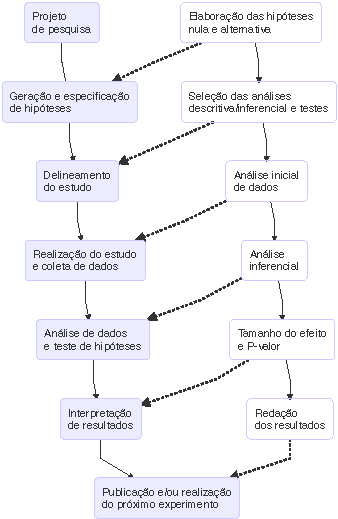
\includegraphics{Ciencia-com-R_files/figure-latex/unnamed-chunk-1-1} 

}

\caption{Mapa mental da relação entre o pensamento estatístico e o pensamento metodológico.}\label{fig:unnamed-chunk-1}
\end{figure}

\hypertarget{como-selecionar-os-testes-para-a-anuxe1lise-estatuxedstica-inferencial}{%
\subsection{Como selecionar os testes para a análise estatística inferencial?}\label{como-selecionar-os-testes-para-a-anuxe1lise-estatuxedstica-inferencial}}

\begin{itemize}
\item
  .\textsuperscript{\protect\hyperlink{ref-dwivedi2019}{123}}
\item
  .\textsuperscript{\protect\hyperlink{ref-Dwivedi2022}{124}}
\item
  .\textsuperscript{\protect\hyperlink{ref-Kim2017}{125}}
\item
  .\textsuperscript{\protect\hyperlink{ref-marusteri2010}{126}}
\item
  .\textsuperscript{\protect\hyperlink{ref-mishra2019}{127}}
\item
  .\textsuperscript{\protect\hyperlink{ref-ray2021}{128}}
\item
  .\textsuperscript{\protect\hyperlink{ref-nayak2011}{129}}
\item
  .\textsuperscript{\protect\hyperlink{ref-shankar2014}{130}}
\end{itemize}

\hypertarget{testes-estatisticos}{%
\chapter{\texorpdfstring{\textbf{Testes estatísticos}}{Testes estatísticos}}\label{testes-estatisticos}}

\hypertarget{teste-de-qui-quadrado-chi2}{%
\section{\texorpdfstring{Teste de Qui-quadrado (\(\chi^2\))}{Teste de Qui-quadrado (\textbackslash chi\^{}2)}}\label{teste-de-qui-quadrado-chi2}}

\begin{Shaded}
\begin{Highlighting}[]
\CommentTok{\# carrega os pacotes}
\FunctionTok{library}\NormalTok{(}\StringTok{"dplyr"}\NormalTok{)}
\FunctionTok{library}\NormalTok{(}\StringTok{"gtsummary"}\NormalTok{)}

\CommentTok{\# tabela 2x2}
\NormalTok{tbl\_cross }\OtherTok{\textless{}{-}} \CommentTok{\# banco de dados tbl\_cross \textless{}{-} \# banco de dados}
\NormalTok{trial }\SpecialCharTok{\%\textgreater{}\%}
    \CommentTok{\# cria a tabela de contingência}
\NormalTok{gtsummary}\SpecialCharTok{::}\FunctionTok{tbl\_cross}\NormalTok{(}\AttributeTok{row =}\NormalTok{ trt, }\AttributeTok{col =}\NormalTok{ response, }\AttributeTok{statistic =} \StringTok{"\{n\}"}\NormalTok{, }\AttributeTok{digits =} \DecValTok{0}\NormalTok{, }\AttributeTok{percent =} \StringTok{"cell"}\NormalTok{,}
    \AttributeTok{margin =} \FunctionTok{c}\NormalTok{(}\StringTok{"row"}\NormalTok{, }\StringTok{"column"}\NormalTok{), }\AttributeTok{missing =} \StringTok{"no"}\NormalTok{, }\AttributeTok{missing\_text =} \StringTok{"Dados perdidos"}\NormalTok{,}
    \AttributeTok{margin\_text =} \StringTok{"Total"}\NormalTok{) }\SpecialCharTok{\%\textgreater{}\%}
    \CommentTok{\# calcula o p{-}valor do teste}
\NormalTok{gtsummary}\SpecialCharTok{::}\FunctionTok{add\_p}\NormalTok{(}\AttributeTok{test =} \StringTok{"chisq.test"}\NormalTok{, }\AttributeTok{pvalue\_fun =} \ControlFlowTok{function}\NormalTok{(x) }\FunctionTok{style\_pvalue}\NormalTok{(x, }\AttributeTok{digits =} \DecValTok{3}\NormalTok{)) }\SpecialCharTok{\%\textgreater{}\%}
\NormalTok{    gtsummary}\SpecialCharTok{::}\FunctionTok{modify\_header}\NormalTok{(}\AttributeTok{p.value =} \StringTok{"**P{-}valor**"}\NormalTok{) }\SpecialCharTok{\%\textgreater{}\%}
    \CommentTok{\# calcula o tamanho do efeito}
\NormalTok{gtsummary}\SpecialCharTok{::}\FunctionTok{modify\_table\_styling}\NormalTok{(}\AttributeTok{rows =} \ConstantTok{NULL}\NormalTok{, }\AttributeTok{footnote =} \FunctionTok{as.character}\NormalTok{(rstatix}\SpecialCharTok{::}\FunctionTok{cramer\_v}\NormalTok{(trt,}
\NormalTok{    response))) }\SpecialCharTok{\%\textgreater{}\%}
    \CommentTok{\# formata o título em negrito}
\NormalTok{gtsummary}\SpecialCharTok{::}\FunctionTok{bold\_labels}\NormalTok{() }\SpecialCharTok{\%\textgreater{}\%}
    \CommentTok{\# cria título da tabela}
\NormalTok{gtsummary}\SpecialCharTok{::}\FunctionTok{modify\_caption}\NormalTok{(}\StringTok{"Teste Qui{-}quadrado (com correção de Yates)"}\NormalTok{)}

\CommentTok{\# exibe a tabela}
\NormalTok{tbl\_cross }\SpecialCharTok{\%\textgreater{}\%}
\NormalTok{    gtsummary}\SpecialCharTok{::}\FunctionTok{as\_hux\_table}\NormalTok{()}
\end{Highlighting}
\end{Shaded}

 
  \providecommand{\huxb}[2]{\arrayrulecolor[RGB]{#1}\global\arrayrulewidth=#2pt}
  \providecommand{\huxvb}[2]{\color[RGB]{#1}\vrule width #2pt}
  \providecommand{\huxtpad}[1]{\rule{0pt}{#1}}
  \providecommand{\huxbpad}[1]{\rule[-#1]{0pt}{#1}}

\begin{table}[ht]
\begin{centerbox}
\begin{threeparttable}
\captionsetup{justification=centering,singlelinecheck=off}
\caption{\label{tab:unnamed-chunk-2} Teste Qui-quadrado (com correção de Yates)}
 \setlength{\tabcolsep}{0pt}
\begin{tabular}{l l l l l}


\hhline{}
\arrayrulecolor{black}

\multicolumn{1}{!{\huxvb{0, 0, 0}{0}}l!{\huxvb{0, 0, 0}{0}}}{\huxtpad{6pt + 1em}\raggedright \hspace{6pt} 
 \hspace{6pt}\huxbpad{6pt}} &
\multicolumn{2}{c!{\huxvb{0, 0, 0}{0}}}{\huxtpad{6pt + 1em}\centering \hspace{6pt} \textbf{Tumor Response}
 \hspace{6pt}\huxbpad{6pt}} &
\multicolumn{1}{c!{\huxvb{0, 0, 0}{0}}}{\huxtpad{6pt + 1em}\centering \hspace{6pt} 
 \hspace{6pt}\huxbpad{6pt}} &
\multicolumn{1}{c!{\huxvb{0, 0, 0}{0}}}{\huxtpad{6pt + 1em}\centering \hspace{6pt} 
 \hspace{6pt}\huxbpad{6pt}} \tabularnewline[-0.5pt]


\hhline{}
\arrayrulecolor{black}

\multicolumn{1}{!{\huxvb{0, 0, 0}{0}}l!{\huxvb{0, 0, 0}{0}}}{\huxtpad{6pt + 1em}\raggedright \hspace{6pt} 
 \hspace{6pt}\huxbpad{6pt}} &
\multicolumn{1}{c!{\huxvb{0, 0, 0}{0}}}{\huxtpad{6pt + 1em}\centering \hspace{6pt} 0
 \hspace{6pt}\huxbpad{6pt}} &
\multicolumn{1}{c!{\huxvb{0, 0, 0}{0}}}{\huxtpad{6pt + 1em}\centering \hspace{6pt} 1
 \hspace{6pt}\huxbpad{6pt}} &
\multicolumn{1}{c!{\huxvb{0, 0, 0}{0}}}{\huxtpad{6pt + 1em}\centering \hspace{6pt} \textbf{Total}
 \hspace{6pt}\huxbpad{6pt}} &
\multicolumn{1}{c!{\huxvb{0, 0, 0}{0}}}{\huxtpad{6pt + 1em}\centering \hspace{6pt} \textbf{\textbf{P-valor}}
 \hspace{6pt}\huxbpad{6pt}} \tabularnewline[-0.5pt]


\hhline{>{\huxb{0, 0, 0}{0.4}}->{\huxb{0, 0, 0}{0.4}}->{\huxb{0, 0, 0}{0.4}}->{\huxb{0, 0, 0}{0.4}}->{\huxb{0, 0, 0}{0.4}}-}
\arrayrulecolor{black}

\multicolumn{1}{!{\huxvb{0, 0, 0}{0}}l!{\huxvb{0, 0, 0}{0}}}{\huxtpad{6pt + 1em}\raggedright \hspace{6pt} \textbf{Chemotherapy Treatment} \hspace{6pt}\huxbpad{6pt}} &
\multicolumn{1}{c!{\huxvb{0, 0, 0}{0}}}{\huxtpad{6pt + 1em}\centering \hspace{6pt}  \hspace{6pt}\huxbpad{6pt}} &
\multicolumn{1}{c!{\huxvb{0, 0, 0}{0}}}{\huxtpad{6pt + 1em}\centering \hspace{6pt}  \hspace{6pt}\huxbpad{6pt}} &
\multicolumn{1}{c!{\huxvb{0, 0, 0}{0}}}{\huxtpad{6pt + 1em}\centering \hspace{6pt}  \hspace{6pt}\huxbpad{6pt}} &
\multicolumn{1}{c!{\huxvb{0, 0, 0}{0}}}{\huxtpad{6pt + 1em}\centering \hspace{6pt} 0.637 \hspace{6pt}\huxbpad{6pt}} \tabularnewline[-0.5pt]


\hhline{}
\arrayrulecolor{black}

\multicolumn{1}{!{\huxvb{0, 0, 0}{0}}l!{\huxvb{0, 0, 0}{0}}}{\huxtpad{6pt + 1em}\raggedright \hspace{15pt} Drug A \hspace{6pt}\huxbpad{6pt}} &
\multicolumn{1}{c!{\huxvb{0, 0, 0}{0}}}{\huxtpad{6pt + 1em}\centering \hspace{6pt} 67 \hspace{6pt}\huxbpad{6pt}} &
\multicolumn{1}{c!{\huxvb{0, 0, 0}{0}}}{\huxtpad{6pt + 1em}\centering \hspace{6pt} 28 \hspace{6pt}\huxbpad{6pt}} &
\multicolumn{1}{c!{\huxvb{0, 0, 0}{0}}}{\huxtpad{6pt + 1em}\centering \hspace{6pt} 95 \hspace{6pt}\huxbpad{6pt}} &
\multicolumn{1}{c!{\huxvb{0, 0, 0}{0}}}{\huxtpad{6pt + 1em}\centering \hspace{6pt}  \hspace{6pt}\huxbpad{6pt}} \tabularnewline[-0.5pt]


\hhline{}
\arrayrulecolor{black}

\multicolumn{1}{!{\huxvb{0, 0, 0}{0}}l!{\huxvb{0, 0, 0}{0}}}{\huxtpad{6pt + 1em}\raggedright \hspace{15pt} Drug B \hspace{6pt}\huxbpad{6pt}} &
\multicolumn{1}{c!{\huxvb{0, 0, 0}{0}}}{\huxtpad{6pt + 1em}\centering \hspace{6pt} 65 \hspace{6pt}\huxbpad{6pt}} &
\multicolumn{1}{c!{\huxvb{0, 0, 0}{0}}}{\huxtpad{6pt + 1em}\centering \hspace{6pt} 33 \hspace{6pt}\huxbpad{6pt}} &
\multicolumn{1}{c!{\huxvb{0, 0, 0}{0}}}{\huxtpad{6pt + 1em}\centering \hspace{6pt} 98 \hspace{6pt}\huxbpad{6pt}} &
\multicolumn{1}{c!{\huxvb{0, 0, 0}{0}}}{\huxtpad{6pt + 1em}\centering \hspace{6pt}  \hspace{6pt}\huxbpad{6pt}} \tabularnewline[-0.5pt]


\hhline{}
\arrayrulecolor{black}

\multicolumn{1}{!{\huxvb{0, 0, 0}{0}}l!{\huxvb{0, 0, 0}{0}}}{\huxtpad{6pt + 1em}\raggedright \hspace{6pt} \textbf{Total} \hspace{6pt}\huxbpad{6pt}} &
\multicolumn{1}{c!{\huxvb{0, 0, 0}{0}}}{\huxtpad{6pt + 1em}\centering \hspace{6pt} 132 \hspace{6pt}\huxbpad{6pt}} &
\multicolumn{1}{c!{\huxvb{0, 0, 0}{0}}}{\huxtpad{6pt + 1em}\centering \hspace{6pt} 61 \hspace{6pt}\huxbpad{6pt}} &
\multicolumn{1}{c!{\huxvb{0, 0, 0}{0}}}{\huxtpad{6pt + 1em}\centering \hspace{6pt} 193 \hspace{6pt}\huxbpad{6pt}} &
\multicolumn{1}{c!{\huxvb{0, 0, 0}{0}}}{\huxtpad{6pt + 1em}\centering \hspace{6pt}  \hspace{6pt}\huxbpad{6pt}} \tabularnewline[-0.5pt]


\hhline{>{\huxb{0, 0, 0}{0.8}}->{\huxb{0, 0, 0}{0.8}}->{\huxb{0, 0, 0}{0.8}}->{\huxb{0, 0, 0}{0.8}}->{\huxb{0, 0, 0}{0.8}}-}
\arrayrulecolor{black}

\multicolumn{5}{!{\huxvb{0, 0, 0}{0}}l!{\huxvb{0, 0, 0}{0}}}{\huxtpad{6pt + 1em}\raggedright \hspace{6pt} Pearson's Chi-squared test \hspace{6pt}\huxbpad{6pt}} \tabularnewline[-0.5pt]


\hhline{}
\arrayrulecolor{black}
\end{tabular}
\end{threeparttable}\par\end{centerbox}

\end{table}
 

\begin{Shaded}
\begin{Highlighting}[]
\CommentTok{\# carrega os pacotes}
\FunctionTok{library}\NormalTok{(}\StringTok{"dplyr"}\NormalTok{)}
\FunctionTok{library}\NormalTok{(}\StringTok{"gtsummary"}\NormalTok{)}

\CommentTok{\# tabela 2x2}
\NormalTok{tbl\_cross }\OtherTok{\textless{}{-}} \CommentTok{\# banco de dados tbl\_cross \textless{}{-} \# banco de dados}
\NormalTok{trial }\SpecialCharTok{\%\textgreater{}\%}
    \CommentTok{\# cria a tabela de contingência}
\NormalTok{gtsummary}\SpecialCharTok{::}\FunctionTok{tbl\_cross}\NormalTok{(}\AttributeTok{row =}\NormalTok{ trt, }\AttributeTok{col =}\NormalTok{ response, }\AttributeTok{statistic =} \StringTok{"\{n\}"}\NormalTok{, }\AttributeTok{digits =} \DecValTok{0}\NormalTok{, }\AttributeTok{percent =} \StringTok{"cell"}\NormalTok{,}
    \AttributeTok{margin =} \FunctionTok{c}\NormalTok{(}\StringTok{"row"}\NormalTok{, }\StringTok{"column"}\NormalTok{), }\AttributeTok{missing =} \StringTok{"no"}\NormalTok{, }\AttributeTok{missing\_text =} \StringTok{"Dados perdidos"}\NormalTok{,}
    \AttributeTok{margin\_text =} \StringTok{"Total"}\NormalTok{) }\SpecialCharTok{\%\textgreater{}\%}
    \CommentTok{\# calcula o p{-}valor do teste}
\NormalTok{gtsummary}\SpecialCharTok{::}\FunctionTok{add\_p}\NormalTok{(}\AttributeTok{test =} \StringTok{"chisq.test.no.correct"}\NormalTok{, }\AttributeTok{pvalue\_fun =} \ControlFlowTok{function}\NormalTok{(x) }\FunctionTok{style\_pvalue}\NormalTok{(x,}
    \AttributeTok{digits =} \DecValTok{3}\NormalTok{)) }\SpecialCharTok{\%\textgreater{}\%}
\NormalTok{    gtsummary}\SpecialCharTok{::}\FunctionTok{modify\_header}\NormalTok{(}\AttributeTok{p.value =} \StringTok{"**P{-}valor**"}\NormalTok{) }\SpecialCharTok{\%\textgreater{}\%}
    \CommentTok{\# calcula o tamanho do efeito}
\NormalTok{gtsummary}\SpecialCharTok{::}\FunctionTok{modify\_table\_styling}\NormalTok{(}\AttributeTok{rows =} \ConstantTok{NULL}\NormalTok{, }\AttributeTok{footnote =} \FunctionTok{as.character}\NormalTok{(rstatix}\SpecialCharTok{::}\FunctionTok{cramer\_v}\NormalTok{(trt,}
\NormalTok{    response))) }\SpecialCharTok{\%\textgreater{}\%}
    \CommentTok{\# formata o título em negrito}
\NormalTok{gtsummary}\SpecialCharTok{::}\FunctionTok{bold\_labels}\NormalTok{() }\SpecialCharTok{\%\textgreater{}\%}
    \CommentTok{\# cria título da tabela}
\NormalTok{gtsummary}\SpecialCharTok{::}\FunctionTok{modify\_caption}\NormalTok{(}\StringTok{"Teste Qui{-}quadrado (sem correção de Yates)"}\NormalTok{)}

\CommentTok{\# exibe a tabela}
\NormalTok{tbl\_cross }\SpecialCharTok{\%\textgreater{}\%}
\NormalTok{    gtsummary}\SpecialCharTok{::}\FunctionTok{as\_hux\_table}\NormalTok{()}
\end{Highlighting}
\end{Shaded}

 
  \providecommand{\huxb}[2]{\arrayrulecolor[RGB]{#1}\global\arrayrulewidth=#2pt}
  \providecommand{\huxvb}[2]{\color[RGB]{#1}\vrule width #2pt}
  \providecommand{\huxtpad}[1]{\rule{0pt}{#1}}
  \providecommand{\huxbpad}[1]{\rule[-#1]{0pt}{#1}}

\begin{table}[ht]
\begin{centerbox}
\begin{threeparttable}
\captionsetup{justification=centering,singlelinecheck=off}
\caption{\label{tab:unnamed-chunk-3} Teste Qui-quadrado (sem correção de Yates)}
 \setlength{\tabcolsep}{0pt}
\begin{tabular}{l l l l l}


\hhline{}
\arrayrulecolor{black}

\multicolumn{1}{!{\huxvb{0, 0, 0}{0}}l!{\huxvb{0, 0, 0}{0}}}{\huxtpad{6pt + 1em}\raggedright \hspace{6pt} 
 \hspace{6pt}\huxbpad{6pt}} &
\multicolumn{2}{c!{\huxvb{0, 0, 0}{0}}}{\huxtpad{6pt + 1em}\centering \hspace{6pt} \textbf{Tumor Response}
 \hspace{6pt}\huxbpad{6pt}} &
\multicolumn{1}{c!{\huxvb{0, 0, 0}{0}}}{\huxtpad{6pt + 1em}\centering \hspace{6pt} 
 \hspace{6pt}\huxbpad{6pt}} &
\multicolumn{1}{c!{\huxvb{0, 0, 0}{0}}}{\huxtpad{6pt + 1em}\centering \hspace{6pt} 
 \hspace{6pt}\huxbpad{6pt}} \tabularnewline[-0.5pt]


\hhline{}
\arrayrulecolor{black}

\multicolumn{1}{!{\huxvb{0, 0, 0}{0}}l!{\huxvb{0, 0, 0}{0}}}{\huxtpad{6pt + 1em}\raggedright \hspace{6pt} 
 \hspace{6pt}\huxbpad{6pt}} &
\multicolumn{1}{c!{\huxvb{0, 0, 0}{0}}}{\huxtpad{6pt + 1em}\centering \hspace{6pt} 0
 \hspace{6pt}\huxbpad{6pt}} &
\multicolumn{1}{c!{\huxvb{0, 0, 0}{0}}}{\huxtpad{6pt + 1em}\centering \hspace{6pt} 1
 \hspace{6pt}\huxbpad{6pt}} &
\multicolumn{1}{c!{\huxvb{0, 0, 0}{0}}}{\huxtpad{6pt + 1em}\centering \hspace{6pt} \textbf{Total}
 \hspace{6pt}\huxbpad{6pt}} &
\multicolumn{1}{c!{\huxvb{0, 0, 0}{0}}}{\huxtpad{6pt + 1em}\centering \hspace{6pt} \textbf{\textbf{P-valor}}
 \hspace{6pt}\huxbpad{6pt}} \tabularnewline[-0.5pt]


\hhline{>{\huxb{0, 0, 0}{0.4}}->{\huxb{0, 0, 0}{0.4}}->{\huxb{0, 0, 0}{0.4}}->{\huxb{0, 0, 0}{0.4}}->{\huxb{0, 0, 0}{0.4}}-}
\arrayrulecolor{black}

\multicolumn{1}{!{\huxvb{0, 0, 0}{0}}l!{\huxvb{0, 0, 0}{0}}}{\huxtpad{6pt + 1em}\raggedright \hspace{6pt} \textbf{Chemotherapy Treatment} \hspace{6pt}\huxbpad{6pt}} &
\multicolumn{1}{c!{\huxvb{0, 0, 0}{0}}}{\huxtpad{6pt + 1em}\centering \hspace{6pt}  \hspace{6pt}\huxbpad{6pt}} &
\multicolumn{1}{c!{\huxvb{0, 0, 0}{0}}}{\huxtpad{6pt + 1em}\centering \hspace{6pt}  \hspace{6pt}\huxbpad{6pt}} &
\multicolumn{1}{c!{\huxvb{0, 0, 0}{0}}}{\huxtpad{6pt + 1em}\centering \hspace{6pt}  \hspace{6pt}\huxbpad{6pt}} &
\multicolumn{1}{c!{\huxvb{0, 0, 0}{0}}}{\huxtpad{6pt + 1em}\centering \hspace{6pt} 0.530 \hspace{6pt}\huxbpad{6pt}} \tabularnewline[-0.5pt]


\hhline{}
\arrayrulecolor{black}

\multicolumn{1}{!{\huxvb{0, 0, 0}{0}}l!{\huxvb{0, 0, 0}{0}}}{\huxtpad{6pt + 1em}\raggedright \hspace{15pt} Drug A \hspace{6pt}\huxbpad{6pt}} &
\multicolumn{1}{c!{\huxvb{0, 0, 0}{0}}}{\huxtpad{6pt + 1em}\centering \hspace{6pt} 67 \hspace{6pt}\huxbpad{6pt}} &
\multicolumn{1}{c!{\huxvb{0, 0, 0}{0}}}{\huxtpad{6pt + 1em}\centering \hspace{6pt} 28 \hspace{6pt}\huxbpad{6pt}} &
\multicolumn{1}{c!{\huxvb{0, 0, 0}{0}}}{\huxtpad{6pt + 1em}\centering \hspace{6pt} 95 \hspace{6pt}\huxbpad{6pt}} &
\multicolumn{1}{c!{\huxvb{0, 0, 0}{0}}}{\huxtpad{6pt + 1em}\centering \hspace{6pt}  \hspace{6pt}\huxbpad{6pt}} \tabularnewline[-0.5pt]


\hhline{}
\arrayrulecolor{black}

\multicolumn{1}{!{\huxvb{0, 0, 0}{0}}l!{\huxvb{0, 0, 0}{0}}}{\huxtpad{6pt + 1em}\raggedright \hspace{15pt} Drug B \hspace{6pt}\huxbpad{6pt}} &
\multicolumn{1}{c!{\huxvb{0, 0, 0}{0}}}{\huxtpad{6pt + 1em}\centering \hspace{6pt} 65 \hspace{6pt}\huxbpad{6pt}} &
\multicolumn{1}{c!{\huxvb{0, 0, 0}{0}}}{\huxtpad{6pt + 1em}\centering \hspace{6pt} 33 \hspace{6pt}\huxbpad{6pt}} &
\multicolumn{1}{c!{\huxvb{0, 0, 0}{0}}}{\huxtpad{6pt + 1em}\centering \hspace{6pt} 98 \hspace{6pt}\huxbpad{6pt}} &
\multicolumn{1}{c!{\huxvb{0, 0, 0}{0}}}{\huxtpad{6pt + 1em}\centering \hspace{6pt}  \hspace{6pt}\huxbpad{6pt}} \tabularnewline[-0.5pt]


\hhline{}
\arrayrulecolor{black}

\multicolumn{1}{!{\huxvb{0, 0, 0}{0}}l!{\huxvb{0, 0, 0}{0}}}{\huxtpad{6pt + 1em}\raggedright \hspace{6pt} \textbf{Total} \hspace{6pt}\huxbpad{6pt}} &
\multicolumn{1}{c!{\huxvb{0, 0, 0}{0}}}{\huxtpad{6pt + 1em}\centering \hspace{6pt} 132 \hspace{6pt}\huxbpad{6pt}} &
\multicolumn{1}{c!{\huxvb{0, 0, 0}{0}}}{\huxtpad{6pt + 1em}\centering \hspace{6pt} 61 \hspace{6pt}\huxbpad{6pt}} &
\multicolumn{1}{c!{\huxvb{0, 0, 0}{0}}}{\huxtpad{6pt + 1em}\centering \hspace{6pt} 193 \hspace{6pt}\huxbpad{6pt}} &
\multicolumn{1}{c!{\huxvb{0, 0, 0}{0}}}{\huxtpad{6pt + 1em}\centering \hspace{6pt}  \hspace{6pt}\huxbpad{6pt}} \tabularnewline[-0.5pt]


\hhline{>{\huxb{0, 0, 0}{0.8}}->{\huxb{0, 0, 0}{0.8}}->{\huxb{0, 0, 0}{0.8}}->{\huxb{0, 0, 0}{0.8}}->{\huxb{0, 0, 0}{0.8}}-}
\arrayrulecolor{black}

\multicolumn{5}{!{\huxvb{0, 0, 0}{0}}l!{\huxvb{0, 0, 0}{0}}}{\huxtpad{6pt + 1em}\raggedright \hspace{6pt} Pearson's Chi-squared test \hspace{6pt}\huxbpad{6pt}} \tabularnewline[-0.5pt]


\hhline{}
\arrayrulecolor{black}
\end{tabular}
\end{threeparttable}\par\end{centerbox}

\end{table}
 

\hypertarget{teste-exato-de-fisher}{%
\section{Teste exato de Fisher}\label{teste-exato-de-fisher}}

\begin{Shaded}
\begin{Highlighting}[]
\CommentTok{\# carrega os pacotes}
\FunctionTok{library}\NormalTok{(}\StringTok{"dplyr"}\NormalTok{)}
\FunctionTok{library}\NormalTok{(}\StringTok{"gtsummary"}\NormalTok{)}

\CommentTok{\# tabela 2x2}
\NormalTok{tbl\_cross }\OtherTok{\textless{}{-}} \CommentTok{\# banco de dados tbl\_cross \textless{}{-} \# banco de dados}
\NormalTok{trial }\SpecialCharTok{\%\textgreater{}\%}
    \CommentTok{\# cria a tabela de contingência}
\NormalTok{gtsummary}\SpecialCharTok{::}\FunctionTok{tbl\_cross}\NormalTok{(}\AttributeTok{row =}\NormalTok{ trt, }\AttributeTok{col =}\NormalTok{ response, }\AttributeTok{statistic =} \StringTok{"\{n\}"}\NormalTok{, }\AttributeTok{digits =} \DecValTok{0}\NormalTok{, }\AttributeTok{percent =} \StringTok{"cell"}\NormalTok{,}
    \AttributeTok{margin =} \FunctionTok{c}\NormalTok{(}\StringTok{"row"}\NormalTok{, }\StringTok{"column"}\NormalTok{), }\AttributeTok{missing =} \StringTok{"no"}\NormalTok{, }\AttributeTok{missing\_text =} \StringTok{"Dados perdidos"}\NormalTok{,}
    \AttributeTok{margin\_text =} \StringTok{"Total"}\NormalTok{) }\SpecialCharTok{\%\textgreater{}\%}
    \CommentTok{\# calcula o p{-}valor do teste}
\NormalTok{gtsummary}\SpecialCharTok{::}\FunctionTok{add\_p}\NormalTok{(}\AttributeTok{test =} \StringTok{"fisher.test"}\NormalTok{, }\AttributeTok{pvalue\_fun =} \ControlFlowTok{function}\NormalTok{(x) }\FunctionTok{style\_pvalue}\NormalTok{(x, }\AttributeTok{digits =} \DecValTok{3}\NormalTok{)) }\SpecialCharTok{\%\textgreater{}\%}
\NormalTok{    gtsummary}\SpecialCharTok{::}\FunctionTok{modify\_header}\NormalTok{(}\AttributeTok{p.value =} \StringTok{"**P{-}valor**"}\NormalTok{) }\SpecialCharTok{\%\textgreater{}\%}
    \CommentTok{\# calcula o tamanho do efeito}
\NormalTok{gtsummary}\SpecialCharTok{::}\FunctionTok{modify\_table\_styling}\NormalTok{(}\AttributeTok{rows =} \ConstantTok{NULL}\NormalTok{, }\AttributeTok{footnote =} \FunctionTok{as.character}\NormalTok{(rstatix}\SpecialCharTok{::}\FunctionTok{cramer\_v}\NormalTok{(trt,}
\NormalTok{    response))) }\SpecialCharTok{\%\textgreater{}\%}
    \CommentTok{\# formata o título em negrito}
\NormalTok{gtsummary}\SpecialCharTok{::}\FunctionTok{bold\_labels}\NormalTok{() }\SpecialCharTok{\%\textgreater{}\%}
    \CommentTok{\# cria título da tabela}
\NormalTok{gtsummary}\SpecialCharTok{::}\FunctionTok{modify\_caption}\NormalTok{(}\StringTok{"Teste exato de Fisher"}\NormalTok{)}

\CommentTok{\# exibe a tabela}
\NormalTok{tbl\_cross }\SpecialCharTok{\%\textgreater{}\%}
\NormalTok{    gtsummary}\SpecialCharTok{::}\FunctionTok{as\_hux\_table}\NormalTok{()}
\end{Highlighting}
\end{Shaded}

 
  \providecommand{\huxb}[2]{\arrayrulecolor[RGB]{#1}\global\arrayrulewidth=#2pt}
  \providecommand{\huxvb}[2]{\color[RGB]{#1}\vrule width #2pt}
  \providecommand{\huxtpad}[1]{\rule{0pt}{#1}}
  \providecommand{\huxbpad}[1]{\rule[-#1]{0pt}{#1}}

\begin{table}[ht]
\begin{centerbox}
\begin{threeparttable}
\captionsetup{justification=centering,singlelinecheck=off}
\caption{\label{tab:unnamed-chunk-4} Teste exato de Fisher}
 \setlength{\tabcolsep}{0pt}
\begin{tabular}{l l l l l}


\hhline{}
\arrayrulecolor{black}

\multicolumn{1}{!{\huxvb{0, 0, 0}{0}}l!{\huxvb{0, 0, 0}{0}}}{\huxtpad{6pt + 1em}\raggedright \hspace{6pt} 
 \hspace{6pt}\huxbpad{6pt}} &
\multicolumn{2}{c!{\huxvb{0, 0, 0}{0}}}{\huxtpad{6pt + 1em}\centering \hspace{6pt} \textbf{Tumor Response}
 \hspace{6pt}\huxbpad{6pt}} &
\multicolumn{1}{c!{\huxvb{0, 0, 0}{0}}}{\huxtpad{6pt + 1em}\centering \hspace{6pt} 
 \hspace{6pt}\huxbpad{6pt}} &
\multicolumn{1}{c!{\huxvb{0, 0, 0}{0}}}{\huxtpad{6pt + 1em}\centering \hspace{6pt} 
 \hspace{6pt}\huxbpad{6pt}} \tabularnewline[-0.5pt]


\hhline{}
\arrayrulecolor{black}

\multicolumn{1}{!{\huxvb{0, 0, 0}{0}}l!{\huxvb{0, 0, 0}{0}}}{\huxtpad{6pt + 1em}\raggedright \hspace{6pt} 
 \hspace{6pt}\huxbpad{6pt}} &
\multicolumn{1}{c!{\huxvb{0, 0, 0}{0}}}{\huxtpad{6pt + 1em}\centering \hspace{6pt} 0
 \hspace{6pt}\huxbpad{6pt}} &
\multicolumn{1}{c!{\huxvb{0, 0, 0}{0}}}{\huxtpad{6pt + 1em}\centering \hspace{6pt} 1
 \hspace{6pt}\huxbpad{6pt}} &
\multicolumn{1}{c!{\huxvb{0, 0, 0}{0}}}{\huxtpad{6pt + 1em}\centering \hspace{6pt} \textbf{Total}
 \hspace{6pt}\huxbpad{6pt}} &
\multicolumn{1}{c!{\huxvb{0, 0, 0}{0}}}{\huxtpad{6pt + 1em}\centering \hspace{6pt} \textbf{\textbf{P-valor}}
 \hspace{6pt}\huxbpad{6pt}} \tabularnewline[-0.5pt]


\hhline{>{\huxb{0, 0, 0}{0.4}}->{\huxb{0, 0, 0}{0.4}}->{\huxb{0, 0, 0}{0.4}}->{\huxb{0, 0, 0}{0.4}}->{\huxb{0, 0, 0}{0.4}}-}
\arrayrulecolor{black}

\multicolumn{1}{!{\huxvb{0, 0, 0}{0}}l!{\huxvb{0, 0, 0}{0}}}{\huxtpad{6pt + 1em}\raggedright \hspace{6pt} \textbf{Chemotherapy Treatment} \hspace{6pt}\huxbpad{6pt}} &
\multicolumn{1}{c!{\huxvb{0, 0, 0}{0}}}{\huxtpad{6pt + 1em}\centering \hspace{6pt}  \hspace{6pt}\huxbpad{6pt}} &
\multicolumn{1}{c!{\huxvb{0, 0, 0}{0}}}{\huxtpad{6pt + 1em}\centering \hspace{6pt}  \hspace{6pt}\huxbpad{6pt}} &
\multicolumn{1}{c!{\huxvb{0, 0, 0}{0}}}{\huxtpad{6pt + 1em}\centering \hspace{6pt}  \hspace{6pt}\huxbpad{6pt}} &
\multicolumn{1}{c!{\huxvb{0, 0, 0}{0}}}{\huxtpad{6pt + 1em}\centering \hspace{6pt} 0.540 \hspace{6pt}\huxbpad{6pt}} \tabularnewline[-0.5pt]


\hhline{}
\arrayrulecolor{black}

\multicolumn{1}{!{\huxvb{0, 0, 0}{0}}l!{\huxvb{0, 0, 0}{0}}}{\huxtpad{6pt + 1em}\raggedright \hspace{15pt} Drug A \hspace{6pt}\huxbpad{6pt}} &
\multicolumn{1}{c!{\huxvb{0, 0, 0}{0}}}{\huxtpad{6pt + 1em}\centering \hspace{6pt} 67 \hspace{6pt}\huxbpad{6pt}} &
\multicolumn{1}{c!{\huxvb{0, 0, 0}{0}}}{\huxtpad{6pt + 1em}\centering \hspace{6pt} 28 \hspace{6pt}\huxbpad{6pt}} &
\multicolumn{1}{c!{\huxvb{0, 0, 0}{0}}}{\huxtpad{6pt + 1em}\centering \hspace{6pt} 95 \hspace{6pt}\huxbpad{6pt}} &
\multicolumn{1}{c!{\huxvb{0, 0, 0}{0}}}{\huxtpad{6pt + 1em}\centering \hspace{6pt}  \hspace{6pt}\huxbpad{6pt}} \tabularnewline[-0.5pt]


\hhline{}
\arrayrulecolor{black}

\multicolumn{1}{!{\huxvb{0, 0, 0}{0}}l!{\huxvb{0, 0, 0}{0}}}{\huxtpad{6pt + 1em}\raggedright \hspace{15pt} Drug B \hspace{6pt}\huxbpad{6pt}} &
\multicolumn{1}{c!{\huxvb{0, 0, 0}{0}}}{\huxtpad{6pt + 1em}\centering \hspace{6pt} 65 \hspace{6pt}\huxbpad{6pt}} &
\multicolumn{1}{c!{\huxvb{0, 0, 0}{0}}}{\huxtpad{6pt + 1em}\centering \hspace{6pt} 33 \hspace{6pt}\huxbpad{6pt}} &
\multicolumn{1}{c!{\huxvb{0, 0, 0}{0}}}{\huxtpad{6pt + 1em}\centering \hspace{6pt} 98 \hspace{6pt}\huxbpad{6pt}} &
\multicolumn{1}{c!{\huxvb{0, 0, 0}{0}}}{\huxtpad{6pt + 1em}\centering \hspace{6pt}  \hspace{6pt}\huxbpad{6pt}} \tabularnewline[-0.5pt]


\hhline{}
\arrayrulecolor{black}

\multicolumn{1}{!{\huxvb{0, 0, 0}{0}}l!{\huxvb{0, 0, 0}{0}}}{\huxtpad{6pt + 1em}\raggedright \hspace{6pt} \textbf{Total} \hspace{6pt}\huxbpad{6pt}} &
\multicolumn{1}{c!{\huxvb{0, 0, 0}{0}}}{\huxtpad{6pt + 1em}\centering \hspace{6pt} 132 \hspace{6pt}\huxbpad{6pt}} &
\multicolumn{1}{c!{\huxvb{0, 0, 0}{0}}}{\huxtpad{6pt + 1em}\centering \hspace{6pt} 61 \hspace{6pt}\huxbpad{6pt}} &
\multicolumn{1}{c!{\huxvb{0, 0, 0}{0}}}{\huxtpad{6pt + 1em}\centering \hspace{6pt} 193 \hspace{6pt}\huxbpad{6pt}} &
\multicolumn{1}{c!{\huxvb{0, 0, 0}{0}}}{\huxtpad{6pt + 1em}\centering \hspace{6pt}  \hspace{6pt}\huxbpad{6pt}} \tabularnewline[-0.5pt]


\hhline{>{\huxb{0, 0, 0}{0.8}}->{\huxb{0, 0, 0}{0.8}}->{\huxb{0, 0, 0}{0.8}}->{\huxb{0, 0, 0}{0.8}}->{\huxb{0, 0, 0}{0.8}}-}
\arrayrulecolor{black}

\multicolumn{5}{!{\huxvb{0, 0, 0}{0}}l!{\huxvb{0, 0, 0}{0}}}{\huxtpad{6pt + 1em}\raggedright \hspace{6pt} Fisher's exact test \hspace{6pt}\huxbpad{6pt}} \tabularnewline[-0.5pt]


\hhline{}
\arrayrulecolor{black}
\end{tabular}
\end{threeparttable}\par\end{centerbox}

\end{table}
 

\hypertarget{analise-comparacao}{%
\chapter{\texorpdfstring{\textbf{Comparação}}{Comparação}}\label{analise-comparacao}}

\hypertarget{analise-inferencial-comparacao}{%
\section{Análise inferencial de comparação}\label{analise-inferencial-comparacao}}

\hypertarget{o-que-uxe9-anuxe1lise-de-comparauxe7uxe3o-de-dados}{%
\subsection{O que é análise de comparação de dados?}\label{o-que-uxe9-anuxe1lise-de-comparauxe7uxe3o-de-dados}}

\begin{itemize}
\tightlist
\item
  .{[}REF{]}
\end{itemize}

\hypertarget{analise-inferencial-correlacao}{%
\chapter{\texorpdfstring{\textbf{Correlação}}{Correlação}}\label{analise-inferencial-correlacao}}

\hypertarget{analise-correlacao}{%
\section{Análise de correlação}\label{analise-correlacao}}

\hypertarget{o-que-uxe9-anuxe1lise-de-correlauxe7uxe3o}{%
\subsection{O que é análise de correlação?}\label{o-que-uxe9-anuxe1lise-de-correlauxe7uxe3o}}

\begin{itemize}
\tightlist
\item
  .{[}REF{]}
\end{itemize}

\hypertarget{qual-uxe9-a-interpretauxe7uxe3o-das-medidas-de-correlauxe7uxe3o}{%
\subsection{Qual é a interpretação das medidas de correlação?}\label{qual-uxe9-a-interpretauxe7uxe3o-das-medidas-de-correlauxe7uxe3o}}

\begin{itemize}
\item
  Os valores de correlação estão no intervalo \([-1; 1]\).\textsuperscript{\protect\hyperlink{ref-khamis2008}{131},\protect\hyperlink{ref-allison2022}{132}}
\item
  Valores de correlação positivos representam uma relação direta entre as variáveis, tal que valores maiores de uma variável estão associados a valores maiores de outra variável.\textsuperscript{\protect\hyperlink{ref-khamis2008}{131},\protect\hyperlink{ref-allison2022}{132}}
\item
  Valores de correlação negativos representam uma relação indireta (ou inversa) entre as variáveis, tal que valores maiores (menores) de uma variável estão associados a valores maiores (menores) de outra variável.\textsuperscript{\protect\hyperlink{ref-khamis2008}{131},\protect\hyperlink{ref-allison2022}{132}}
\item
  Valores de correlação próximos de \(0\) representam a inexistência de relação entre as variáveis.\textsuperscript{\protect\hyperlink{ref-khamis2008}{131},\protect\hyperlink{ref-allison2022}{132}}
\end{itemize}

\hypertarget{quais-precauuxe7uxf5es-devem-ser-tomadas-na-interpretauxe7uxe3o-de-medidas-de-correlauxe7uxe3o}{%
\subsection{Quais precauções devem ser tomadas na interpretação de medidas de correlação?}\label{quais-precauuxe7uxf5es-devem-ser-tomadas-na-interpretauxe7uxe3o-de-medidas-de-correlauxe7uxe3o}}

\begin{itemize}
\item
  Tamanhos de efeito grande (ou qualquer outro) não representam necessariamente uma relação causa-efeito entre as variáveis.\textsuperscript{\protect\hyperlink{ref-khamis2008}{131}}
\item
  Tamanhos de efeito grande (ou qualquer outro) não representam necessariamente uma relação de concordância ou confiabilidade entre as variáveis.\textsuperscript{\protect\hyperlink{ref-khamis2008}{131}}
\end{itemize}

\hypertarget{quais-testes-podem-ser-usados-para-anuxe1lises-de-correlauxe7uxe3o}{%
\subsection{Quais testes podem ser usados para análises de correlação?}\label{quais-testes-podem-ser-usados-para-anuxe1lises-de-correlauxe7uxe3o}}

\begin{itemize}
\item
  Coeficiente de correlação de Pearson (\(r\)).\textsuperscript{\protect\hyperlink{ref-khamis2008}{131},\protect\hyperlink{ref-allison2022}{132}}

  \begin{itemize}
  \item
    O coeficiente de correlação de Pearson (\(r\)) avalia a força e direção da relação linear entre duas variáveis quantitativas.\textsuperscript{\protect\hyperlink{ref-khamis2008}{131},\protect\hyperlink{ref-allison2022}{132}}
  \item
    Tipo: paramétrico.\textsuperscript{\protect\hyperlink{ref-khamis2008}{131},\protect\hyperlink{ref-allison2022}{132}}
  \item
    Hipóteses:\textsuperscript{\protect\hyperlink{ref-allison2022}{132}}

    \begin{itemize}
    \item
      Nula (\(H_{0}\)): \(r=0\)
    \item
      Alternativa (\(H_{1}\)): \(r≠0\)
    \end{itemize}
  \item
    Tamanho do efeito:\textsuperscript{\protect\hyperlink{ref-khamis2008}{131},\protect\hyperlink{ref-allison2022}{132}}

    \begin{itemize}
    \tightlist
    \item
      Coeficiente de correlação de Pearson (\(r\))
    \end{itemize}
  \end{itemize}
\end{itemize}

\begin{infobox}{images/Rlogo}
O pacote \emph{stats}\textsuperscript{\protect\hyperlink{ref-stats-2}{43}} fornece a função fornece a função \href{https://www.rdocumentation.org/packages/stats/versions/3.6.2/topics/cor.test}{\emph{cor.test}} para calcular o coeficiente de correlação de Pearson (\(r\)).

\end{infobox}

\begin{itemize}
\item
  Coeficiente de correlação ponto-bisserial (\(r_{s}\)).\textsuperscript{\protect\hyperlink{ref-khamis2008}{131}}

  \begin{itemize}
  \item
    O coeficiente de correlação ponto-bisserial (\(r_{s}\)) avalia a força e direção da relação linear entre uma variável quantitativa e outra dicotômica.\textsuperscript{\protect\hyperlink{ref-khamis2008}{131}}
  \item
    Tipo: paramétrico.\textsuperscript{\protect\hyperlink{ref-khamis2008}{131}}
  \item
    Hipóteses:\textsuperscript{\protect\hyperlink{ref-khamis2008}{131}}

    \begin{itemize}
    \item
      Nula (\(H_{0}\)): \(r_{s}=0\)
    \item
      Alternativa (\(H_{1}\)): \(r_{s}≠0\)
    \end{itemize}
  \item
    Tamanho do efeito:\textsuperscript{\protect\hyperlink{ref-khamis2008}{131}}

    \begin{itemize}
    \tightlist
    \item
      Coeficiente de correlação ponto-bisserial (\(r_{s}\))
    \end{itemize}
  \end{itemize}
\end{itemize}

\begin{infobox}{images/Rlogo}
O pacote \emph{stats}\textsuperscript{\protect\hyperlink{ref-stats-2}{43}} fornece a função fornece a função \href{https://www.rdocumentation.org/packages/stats/versions/3.6.2/topics/cor.test}{\emph{cor.test}} para calcular o coeficiente de correlação ponto-bisserial (\(r_{s}\)).

\end{infobox}

\begin{itemize}
\item
  Coeficiente de correlação de Spearman (\(\rho\)).\textsuperscript{\protect\hyperlink{ref-khamis2008}{131},\protect\hyperlink{ref-allison2022}{132}}

  \begin{itemize}
  \item
    O coeficiente de correlação de Spearman (\(\rho\)) avalia a força e direção da relação monotônica entre duas variáveis quantitativas.\textsuperscript{\protect\hyperlink{ref-khamis2008}{131},\protect\hyperlink{ref-allison2022}{132}}
  \item
    O coeficiente de correlação de Spearman (\(\rho\)) pode ser também definida como a correlação de Pearson (\(r\)) entre as classificações (\emph{ranks}) das duas variáveis quantitativas.\textsuperscript{\protect\hyperlink{ref-khamis2008}{131},\protect\hyperlink{ref-allison2022}{132}}
  \item
    Tipo: não-paramétrico.\textsuperscript{\protect\hyperlink{ref-khamis2008}{131},\protect\hyperlink{ref-allison2022}{132}}
  \item
    Hipóteses:\textsuperscript{\protect\hyperlink{ref-khamis2008}{131},\protect\hyperlink{ref-allison2022}{132}}

    \begin{itemize}
    \item
      Nula (\(H_{0}\)): \(\rho=0\)
    \item
      Alternativa (\(H_{1}\)): \(\rho≠0\)
    \end{itemize}
  \item
    Tamanho do efeito:\textsuperscript{\protect\hyperlink{ref-khamis2008}{131},\protect\hyperlink{ref-allison2022}{132}}

    \begin{itemize}
    \tightlist
    \item
      Coeficiente de correlação de Spearman (\(\rho\))
    \end{itemize}
  \end{itemize}
\end{itemize}

\begin{infobox}{images/Rlogo}
O pacote \emph{stats}\textsuperscript{\protect\hyperlink{ref-stats-2}{43}} fornece a função fornece a função \href{https://www.rdocumentation.org/packages/stats/versions/3.6.2/topics/cor.test}{\emph{cor.test}} para calcular o coeficiente de correlação de Spearman (\(\rho\)).

\end{infobox}

\hypertarget{analise-inferencial-associacao}{%
\chapter{\texorpdfstring{\textbf{Associação}}{Associação}}\label{analise-inferencial-associacao}}

\hypertarget{analise-associacao}{%
\section{Análise de associação}\label{analise-associacao}}

\hypertarget{o-que-uxe9-anuxe1lise-de-associauxe7uxe3o}{%
\subsection{O que é análise de associação?}\label{o-que-uxe9-anuxe1lise-de-associauxe7uxe3o}}

\begin{itemize}
\tightlist
\item
  .{[}REF{]}
\end{itemize}

\hypertarget{bivariada}{%
\section{Associação bivariada}\label{bivariada}}

\hypertarget{o-que-suxe3o-anuxe1lises-de-associauxe7uxe3o-bivariada}{%
\subsection{O que são análises de associação bivariada?}\label{o-que-suxe3o-anuxe1lises-de-associauxe7uxe3o-bivariada}}

\begin{itemize}
\tightlist
\item
  .{[}REF{]}
\end{itemize}

\hypertarget{quais-testes-podem-ser-usados-para-anuxe1lises-de-associauxe7uxe3o-bivariada}{%
\subsection{Quais testes podem ser usados para análises de associação bivariada?}\label{quais-testes-podem-ser-usados-para-anuxe1lises-de-associauxe7uxe3o-bivariada}}

\begin{itemize}
\item
  Teste Qui-quadrado (\(\chi^2\)).\textsuperscript{\protect\hyperlink{ref-McHugh2013}{133},\protect\hyperlink{ref-Kim2017a}{134}}

  \begin{itemize}
  \item
    O teste qui-quadrado (\(\chi^2\)) avalia uma hipótese global se a relação entre duas variáveis e/ou fatores é independente ou associada.\textsuperscript{\protect\hyperlink{ref-Kim2017a}{134}}
  \item
    O teste qui-quadrado é utilizado para comparar a distribuição de uma variável categórica em uma amostra ou grupo com a distribuição em outro. Se a distribuição da variável categórica não for muito diferente nos diferentes grupos, pode-se concluir que a distribuição da variável categórica não está relacionada com a variável dos grupos. Pode-se também concluir que a variável categórica e os grupos são independentes.\textsuperscript{\protect\hyperlink{ref-Kim2017a}{134}}
  \item
    Tipo: não paramétrico.\textsuperscript{\protect\hyperlink{ref-McHugh2013}{133},\protect\hyperlink{ref-Kim2017a}{134}}
  \item
    Suposições:\textsuperscript{\protect\hyperlink{ref-McHugh2013}{133},\protect\hyperlink{ref-Kim2017a}{134}}

    \begin{itemize}
    \item
      As variáveis são ordinais ou categóricas nominais, de modo que as células representem frequência.
    \item
      Os níveis dos fatores (variáveis categóricas) são mutuamente exclusivos.
    \item
      Tamanho de amostra grande e adequado porque é baseado em uma abordagem de aproximação.
    \item
      Menos de 20\% das células com frequências esperadas \textless{} 5
    \item
      Nenhuma célula com frequência esperada \textless{} 1.
    \end{itemize}
  \item
    Hipóteses:\textsuperscript{\protect\hyperlink{ref-Kim2017a}{134}}

    \begin{itemize}
    \item
      Nula (\(H_{0}\)): independente (sem associação)
    \item
      Alternativa (\(H_{1}\)): não independente (associação)
    \end{itemize}
  \item
    Tamanho do efeito:\textsuperscript{\protect\hyperlink{ref-Kim2017a}{134}}

    \begin{itemize}
    \item
      Phi (\(\phi\)), para tabelas de contingência 2x2
    \item
      Razão de chances (\(RC\) ou \(OR\)), para tabelas de contingência 2x2
    \item
      Cramer V (\(V\)), para tabelas de contingência NxM
    \end{itemize}
  \end{itemize}
\end{itemize}

\begin{infobox}{images/Rlogo}
O pacote \emph{gtsummary}\textsuperscript{\protect\hyperlink{ref-gtsummary}{135}} fornece a função \href{https://www.rdocumentation.org/packages/gtsummary/versions/1.6.3/topics/tbl_cross}{\emph{tbl\_cross}} para criar uma tabela NxM.

\end{infobox}

\begin{itemize}
\item
  Teste Exato de Fisher (\(\chi^2\)).\textsuperscript{\protect\hyperlink{ref-McHugh2013}{133},\protect\hyperlink{ref-Kim2017a}{134}}

  \begin{itemize}
  \item
    O teste exato de Fisher avalia a hipótese nula de independência aplicando a distribuição hipergeométrica dos números nas células da tabela.\textsuperscript{\protect\hyperlink{ref-Kim2017a}{134}}
  \item
    Hipóteses:\textsuperscript{\protect\hyperlink{ref-McHugh2013}{133},\protect\hyperlink{ref-Kim2017a}{134}}

    \begin{itemize}
    \item
      Nula (\(H_{0}\)): independente (sem associação)
    \item
      Alternativa (\(H_{1}\)): não independente (associação)
    \end{itemize}
  \item
    Tamanho do efeito:\textsuperscript{\protect\hyperlink{ref-McHugh2013}{133},\protect\hyperlink{ref-Kim2017a}{134}}

    \begin{itemize}
    \item
      Phi (\(\phi\)), para tabelas de contingência 2x2
    \item
      Razão de chances (\(RC\) ou \(OR\)), para tabelas de contingência 2x2
    \item
      Cramer V (\(V\)), para tabelas de contingência NxM
    \end{itemize}
  \end{itemize}
\end{itemize}

\begin{infobox}{images/Rlogo}
O pacote \emph{gtsummary}\textsuperscript{\protect\hyperlink{ref-gtsummary}{135}} fornece a função \href{https://www.rdocumentation.org/packages/gtsummary/versions/1.6.3/topics/tbl_cross}{\emph{tbl\_cross}} para criar uma tabela NxM.

\end{infobox}

\begin{itemize}
\item
  Kendall \(\tau\).\textsuperscript{\protect\hyperlink{ref-khamis2008}{131},\protect\hyperlink{ref-allison2022}{132}}

  \begin{itemize}
  \item
    O coeficiente Kendall \(\tau\) avalia a força e direção da relação monotônica entre duas variáveis quantitativas ou qualitativas.\textsuperscript{\protect\hyperlink{ref-khamis2008}{131},\protect\hyperlink{ref-allison2022}{132}}
  \item
    O coeficiente Kendall \(\tau\) é definido como a porporção de todos os pares concordantes menos a proporção de todos os pares discordantes.\textsuperscript{\protect\hyperlink{ref-khamis2008}{131},\protect\hyperlink{ref-allison2022}{132}}
  \item
    Tipo: não-paramétrico.\textsuperscript{\protect\hyperlink{ref-khamis2008}{131},\protect\hyperlink{ref-allison2022}{132}}
  \item
    Hipóteses:\textsuperscript{\protect\hyperlink{ref-khamis2008}{131},\protect\hyperlink{ref-allison2022}{132}}

    \begin{itemize}
    \item
      Nula (\(H_{0}\)): \(\tau=0\)
    \item
      Alternativa (\(H_{1}\)): \(\tau≠0\)
    \end{itemize}
  \item
    Tamanho do efeito:\textsuperscript{\protect\hyperlink{ref-khamis2008}{131},\protect\hyperlink{ref-allison2022}{132}}

    \begin{itemize}
    \tightlist
    \item
      Kendall \(\tau\)
    \end{itemize}
  \end{itemize}
\end{itemize}

\begin{infobox}{images/Rlogo}
O pacote \emph{stats}\textsuperscript{\protect\hyperlink{ref-stats-2}{43}} fornece a função \href{https://www.rdocumentation.org/packages/stats/versions/3.6.2/topics/cor.test}{\emph{cor.test}} para calcular o coeficiente Kendall \(\tau\).

\end{infobox}

\hypertarget{analise-inferencial-regressao}{%
\chapter{\texorpdfstring{\textbf{Regressão}}{Regressão}}\label{analise-inferencial-regressao}}

\hypertarget{analise-regressao}{%
\section{Análise de regressão}\label{analise-regressao}}

\hypertarget{o-que-uxe9-anuxe1lise-de-regressuxe3o}{%
\subsection{O que é análise de regressão?}\label{o-que-uxe9-anuxe1lise-de-regressuxe3o}}

\begin{itemize}
\tightlist
\item
  Para estimar os efeitos imparciais de um fator de exposição primária sobre uma variável de desfecho, frequentemente constroem-se modelos estatísticos de regressão.\textsuperscript{\protect\hyperlink{ref-bandoli2018}{136}}
\end{itemize}

\hypertarget{como-preparar-as-variuxe1veis-categuxf3ricas-para-anuxe1lise-de-regressuxe3o}{%
\subsection{Como preparar as variáveis categóricas para análise de regressão?}\label{como-preparar-as-variuxe1veis-categuxf3ricas-para-anuxe1lise-de-regressuxe3o}}

\begin{itemize}
\item
  Variáveis fictícias (\emph{dummy}) compreendem variáveis criadas para introduzir, nos modelos de regressão, informações contidas em outras variáveis que não podem ser medidas em escala numérica.\textsuperscript{\protect\hyperlink{ref-suits1957}{137}}
\item
  Variáveis categóricas nominais, com 2 ou mais níveis, devem ser subdivididas em variáveis fictícias dicotômicas para ser usada em modelos de regressão.\textsuperscript{\protect\hyperlink{ref-Healy1995}{138}}
\item
  Cada nível da variável categórica nominal será convertido em uma nova variável fictícias dicotômica, tal que a nova variável dicotômica assume valor 1 para a presença do nível correspondente e 0 em qualquer outro caso.\textsuperscript{\protect\hyperlink{ref-Healy1995}{138}}
\end{itemize}

\begin{infobox}{images/Rlogo}
O pacote \emph{fastDummies}\textsuperscript{\protect\hyperlink{ref-fastDummies}{139}} fornece a função \href{https://www.rdocumentation.org/packages/fastDummies/versions/1.7.3/topics/dummy_columns}{\emph{dummy\_cols}} para preparar as variáveis categóricas fictícias para análise de regressão.

\end{infobox}

\hypertarget{multivariavel-multivariada}{%
\section{Regressão simples, multivariável e multivariada}\label{multivariavel-multivariada}}

\hypertarget{o-que-suxe3o-as-anuxe1lises-de-regressuxe3o-simples-multivariuxe1vel-e-multivariada}{%
\subsection{O que são as análises de regressão simples, multivariável e multivariada?}\label{o-que-suxe3o-as-anuxe1lises-de-regressuxe3o-simples-multivariuxe1vel-e-multivariada}}

\begin{itemize}
\item
  A análise de regressão simples consiste em modelos estatísticos com 1 variável dependente (desfecho) e 1 variável independente (preditor).\textsuperscript{\protect\hyperlink{ref-Hidalgo2013}{140}}
\item
  A análise multivariável (ou múltiplo) consiste em modelos estatísticos com 1 variável dependente (desfecho) e duas ou mais variáveis independentes.\textsuperscript{\protect\hyperlink{ref-Hidalgo2013}{140}}
\item
  A análise multivariada consiste em modelos estatísticos com 2 ou mais variáveis dependente (desfechos) e duas ou mais variáveis independentes.\textsuperscript{\protect\hyperlink{ref-Hidalgo2013}{140}}
\end{itemize}

\begin{infobox}{images/Rlogo}
O pacote \emph{modelsummary}\textsuperscript{\protect\hyperlink{ref-modelsummary}{141}} fornece as funções \href{https://www.rdocumentation.org/packages/modelsummary/versions/1.4.1/topics/modelsummary}{\emph{modelsummary}} e \href{https://www.rdocumentation.org/packages/modelsummary/versions/1.4.1/topics/modelplot}{\emph{modelplot}} para gerar tabelas e gráficos de coeficientes de regressão.

\end{infobox}

\hypertarget{quais-testes-podem-ser-usados-em-anuxe1lise-de-associauxe7uxe3o-multivariuxe1vel}{%
\subsection{Quais testes podem ser usados em análise de associação multivariável?}\label{quais-testes-podem-ser-usados-em-anuxe1lise-de-associauxe7uxe3o-multivariuxe1vel}}

\begin{itemize}
\tightlist
\item
  .{[}REF{]}
\end{itemize}

\hypertarget{efeito-principal}{%
\section{Efeito principal}\label{efeito-principal}}

\hypertarget{o-que-uxe9-efeito-principal}{%
\subsection{O que é efeito principal?}\label{o-que-uxe9-efeito-principal}}

\begin{itemize}
\tightlist
\item
  .\textsuperscript{\protect\hyperlink{ref-Bours2023}{142}}
\end{itemize}

\hypertarget{modificacao}{%
\section{Efeito de modificação}\label{modificacao}}

\hypertarget{o-que-uxe9-um-modificador-de-efeito}{%
\subsection{O que é um modificador de efeito?}\label{o-que-uxe9-um-modificador-de-efeito}}

\begin{itemize}
\tightlist
\item
  .\textsuperscript{\protect\hyperlink{ref-Bours2023}{142}}
\end{itemize}

\hypertarget{o-que-uxe9-efeito-de-modificauxe7uxe3o}{%
\subsection{O que é efeito de modificação?}\label{o-que-uxe9-efeito-de-modificauxe7uxe3o}}

\begin{itemize}
\tightlist
\item
  .\textsuperscript{\protect\hyperlink{ref-Bours2023}{142}}
\end{itemize}

\hypertarget{interacao}{%
\section{Efeito de interação}\label{interacao}}

\hypertarget{o-que-uxe9-efeito-de-interauxe7uxe3o}{%
\subsection{O que é efeito de interação?}\label{o-que-uxe9-efeito-de-interauxe7uxe3o}}

\begin{itemize}
\item
  A interação - representada pelo símbolo `*' - é o termo estatístico empregado para representar a heterogeneidade de um determinado efeito.\textsuperscript{\protect\hyperlink{ref-Altman1996}{143}}
\item
  .\textsuperscript{\protect\hyperlink{ref-Bours2023}{142}}
\end{itemize}

\hypertarget{mediacao}{%
\section{Efeito de mediação}\label{mediacao}}

\hypertarget{o-que-uxe9-um-mediador-de-efeito}{%
\subsection{O que é um mediador de efeito?}\label{o-que-uxe9-um-mediador-de-efeito}}

\begin{itemize}
\item
  .\textsuperscript{\protect\hyperlink{ref-Baron1986}{144}}
\item
  .\textsuperscript{\protect\hyperlink{ref-Bours2023}{142}}
\end{itemize}

\hypertarget{o-que-uxe9-efeito-de-mediauxe7uxe3o}{%
\subsection{O que é efeito de mediação?}\label{o-que-uxe9-efeito-de-mediauxe7uxe3o}}

\begin{itemize}
\item
  .\textsuperscript{\protect\hyperlink{ref-Baron1986}{144}}
\item
  .\textsuperscript{\protect\hyperlink{ref-Bours2023}{142}}
\end{itemize}

\hypertarget{o-que-uxe9-efeito-direto}{%
\subsection{O que é efeito direto?}\label{o-que-uxe9-efeito-direto}}

\begin{itemize}
\item
  .\textsuperscript{\protect\hyperlink{ref-Baron1986}{144}}
\item
  .\textsuperscript{\protect\hyperlink{ref-Bours2023}{142}}
\end{itemize}

\hypertarget{o-que-uxe9-efeito-indireto}{%
\subsection{O que é efeito indireto?}\label{o-que-uxe9-efeito-indireto}}

\begin{itemize}
\item
  .\textsuperscript{\protect\hyperlink{ref-Baron1986}{144}}
\item
  .\textsuperscript{\protect\hyperlink{ref-Bours2023}{142}}
\end{itemize}

\hypertarget{o-que-uxe9-efeito-total}{%
\subsection{O que é efeito total?}\label{o-que-uxe9-efeito-total}}

\begin{itemize}
\item
  .\textsuperscript{\protect\hyperlink{ref-Baron1986}{144}}
\item
  .\textsuperscript{\protect\hyperlink{ref-Bours2023}{142}}
\end{itemize}

\hypertarget{selecao}{%
\section{Seleção de variáveis do modelo}\label{selecao}}

\hypertarget{correlauxe7uxe3o-bivariada-pode-ser-usada-para-seleuxe7uxe3o-de-variuxe1veis-em-modelos-de-regressuxe3o-multivariuxe1vel}{%
\subsection{Correlação bivariada pode ser usada para seleção de variáveis em modelos de regressão multivariável?}\label{correlauxe7uxe3o-bivariada-pode-ser-usada-para-seleuxe7uxe3o-de-variuxe1veis-em-modelos-de-regressuxe3o-multivariuxe1vel}}

\begin{itemize}
\item
  Seleção bivariada de variáveis - isto é, aplicação de testes de correlação em pares de variáveis candidatas e variável de desfecho afim de selecionar quais serão incluídas no modelo multivariável - é um dos erros mais comuns na literatura.\textsuperscript{\protect\hyperlink{ref-heinze2016}{118},\protect\hyperlink{ref-Dales1978}{145},\protect\hyperlink{ref-Sun1996}{146}}
\item
  A seleção bivariada de variáveis torna o modelo mais suscetível a otimismo no ajuste se as variáveis de confundimento não são adequadamente controladas.\textsuperscript{\protect\hyperlink{ref-Dales1978}{145},\protect\hyperlink{ref-Sun1996}{146}}
\end{itemize}

\hypertarget{variuxe1veis-sem-significuxe2ncia-estatuxedstica-devem-ser-excluuxeddas-do-modelo-final}{%
\subsection{Variáveis sem significância estatística devem ser excluídas do modelo final?}\label{variuxe1veis-sem-significuxe2ncia-estatuxedstica-devem-ser-excluuxeddas-do-modelo-final}}

\begin{itemize}
\item
  Eliminar uma variável de um modelo significa anular o seu coeficiente de regressão (\(\beta = 0\)), mesmo que o valor estimado pelos dados seja outro. Desta forma, os resultados se afasTAM de uma solução de máxima verossimilhança (que tem fundamento teórico) e o modelo resultante é intencionalmente subótimo.\textsuperscript{\protect\hyperlink{ref-heinze2016}{118}}
\item
  Os coeficientes de regressão geralmente dependem do conjunto de variáveis do modelo e, portanto, podem mudam de valor (``mudança na estimativa'' positiva ou negativa) se uma (ou mais) variável(is) for(em) eliminada(s) do modelo.\textsuperscript{\protect\hyperlink{ref-heinze2016}{118}}
\end{itemize}

\hypertarget{por-que-muxe9todos-de-regressuxe3o-gradual-nuxe3o-suxe3o-recomendados-para-seleuxe7uxe3o-de-variuxe1veis-em-modelos-de-regressuxe3o-multivariuxe1vel}{%
\subsection{Por que métodos de regressão gradual não são recomendados para seleção de variáveis em modelos de regressão multivariável?}\label{por-que-muxe9todos-de-regressuxe3o-gradual-nuxe3o-suxe3o-recomendados-para-seleuxe7uxe3o-de-variuxe1veis-em-modelos-de-regressuxe3o-multivariuxe1vel}}

\begin{itemize}
\item
  Métodos diferentes de regressão gradual podem produzir diferentes seleções de variáveis de um mesmo banco de dados.\textsuperscript{\protect\hyperlink{ref-Healy1995}{138}}
\item
  Nenhum método de regressão gradual garante a seleção ótima de variáveis de um banco de dados.\textsuperscript{\protect\hyperlink{ref-Healy1995}{138}}
\item
  As regras de término da regressão baseadas em p-valor tendem a ser arbitrárias.\textsuperscript{\protect\hyperlink{ref-Healy1995}{138}}
\end{itemize}

\hypertarget{o-que-pode-ser-feito-para-reduzir-o-nuxfamero-de-variuxe1veis-candidatas-em-modelos-de-regressuxe3o-multivariuxe1vel}{%
\subsection{O que pode ser feito para reduzir o número de variáveis candidatas em modelos de regressão multivariável?}\label{o-que-pode-ser-feito-para-reduzir-o-nuxfamero-de-variuxe1veis-candidatas-em-modelos-de-regressuxe3o-multivariuxe1vel}}

\begin{itemize}
\item
  Verifique a existência de multicolinearidade entre as variáveis candidatas.\textsuperscript{\protect\hyperlink{ref-Sun1996}{146}}
\item
  Em caso de uma proporção baixa entre o número de participantes e de variáveis, use o conhecimento prévio da literatura para selecionar um pequeno conjunto de variáveis candidatas.\textsuperscript{\protect\hyperlink{ref-Sun1996}{146}}
\item
  Colapse categorias com contagem nula (células com valor igual a 0) de variáveis candidatas.\textsuperscript{\protect\hyperlink{ref-Sun1996}{146}}
\item
  Use simulações de dados para identificar qual(is) variável(is) está(ão) causando problemas de convergência do ajuste do modelo.\textsuperscript{\protect\hyperlink{ref-Sun1996}{146}}
\item
  A eliminação retroativa tem sido recomendada como a abordagem de regressão gradual mais confiável entre aquelas que podem ser facilmente alcançadas com programas de computador.\textsuperscript{\protect\hyperlink{ref-heinze2016}{118}}
\end{itemize}

\hypertarget{analise-redes}{%
\chapter{\texorpdfstring{\textbf{Redes}}{Redes}}\label{analise-redes}}

\hypertarget{redes}{%
\section{Análise de redes}\label{redes}}

\hypertarget{o-que-uxe9-anuxe1lise-de-rede}{%
\subsection{O que é análise de rede?}\label{o-que-uxe9-anuxe1lise-de-rede}}

\begin{itemize}
\tightlist
\item
  .{[}REF{]}
\end{itemize}

\cftaddtitleline{toc}{chapter}{\rule{\textwidth}{0.4pt}}{}

\hypertarget{parte-3---epidemiologia-aplicada}{%
\chapter*{\texorpdfstring{\textbf{PARTE 3 - Epidemiologia Aplicada}}{PARTE 3 - Epidemiologia Aplicada}}\label{parte-3---epidemiologia-aplicada}}
\addcontentsline{toc}{chapter}{\textbf{PARTE 3 - Epidemiologia Aplicada}}

\markboth{}{}
\par\noindent\rule{\textwidth}{0.05in}

\hypertarget{simulacao-computacional}{%
\chapter{\texorpdfstring{\textbf{Simulação computacional}}{Simulação computacional}}\label{simulacao-computacional}}

\hypertarget{simulacao-computacional-dados}{%
\section{Simulação computacional de dados}\label{simulacao-computacional-dados}}

\hypertarget{o-que-uxe9-simulauxe7uxe3o-computacional-de-dados}{%
\subsection{O que é simulação computacional de dados?}\label{o-que-uxe9-simulauxe7uxe3o-computacional-de-dados}}

\begin{itemize}
\tightlist
\item
  .{[}REF{]}
\end{itemize}

\hypertarget{monte-carlo}{%
\section{Método de Monte Carlo}\label{monte-carlo}}

\hypertarget{o-que-uxe9-o-muxe9todo-de-monte-carlo}{%
\subsection{O que é o método de Monte Carlo?}\label{o-que-uxe9-o-muxe9todo-de-monte-carlo}}

\begin{itemize}
\tightlist
\item
  .{[}REF{]}
\end{itemize}

\hypertarget{estudos-observacionais}{%
\chapter{\texorpdfstring{\textbf{Estudos observacionais}}{Estudos observacionais}}\label{estudos-observacionais}}

\hypertarget{observacionais}{%
\section{Estudos observacionais}\label{observacionais}}

\hypertarget{o-que-uxe9-a-faluxe1cia-da-tabela-2}{%
\subsection{O que é a falácia da Tabela 2?}\label{o-que-uxe9-a-faluxe1cia-da-tabela-2}}

\begin{itemize}
\item
  A Tabela 2 pode induzir ao erro de interpretação pelas estimativas de efeitos para covariáveis do modelo também serem utilizados para controlar a confusão da exposição.\textsuperscript{\protect\hyperlink{ref-Westreich2013}{37},\protect\hyperlink{ref-bandoli2018}{136}}
\item
  Ao apresentar estimativas de efeito ajustadas para covariáveis juntamente com a estimativa de efeito ajustada para a exposição primária, a Tabela 2 sugere implicitamente que todas estas estimativas podem ser interpretadas de forma semelhante, se não de forma idêntica, como estimativa do efeito total.\textsuperscript{\protect\hyperlink{ref-Westreich2013}{37},\protect\hyperlink{ref-bandoli2018}{136}}
\item
  A falácia da Tabela 2 pode ser evitada limitando-se a tabela a estimativas das medidas primárias do efeito de exposição nos diferentes modelos, com as covariáveis secundárias de ``ajuste'' relatadas em uma nota de rodapé, juntamente com a forma como foram categorizadas ou modeladas.\textsuperscript{\protect\hyperlink{ref-Westreich2013}{37}}
\end{itemize}

\hypertarget{ensaio-cluxednico-aleatorizado}{%
\chapter{\texorpdfstring{\textbf{Ensaio clínico aleatorizado}}{Ensaio clínico aleatorizado}}\label{ensaio-cluxednico-aleatorizado}}

\hypertarget{caracteristicas}{%
\section{Características}\label{caracteristicas}}

\hypertarget{quais-suxe3o-as-caracteruxedsticas-dos-ensaios-cluxednicos-aleatorizados}{%
\subsection{Quais são as características dos ensaios clínicos aleatorizados?}\label{quais-suxe3o-as-caracteruxedsticas-dos-ensaios-cluxednicos-aleatorizados}}

\begin{itemize}
\item
  A característica essencial de um ensaio clínico aleatorizado é a comparação entre grupos.\textsuperscript{\protect\hyperlink{ref-bland2011}{147}}
\item
  Quanto à unidade de alocação:\textsuperscript{\protect\hyperlink{ref-Bruce2022}{148}}

  \begin{itemize}
  \item
    Individual
  \item
    Agrupado
  \end{itemize}
\item
  Quanto ao número de braços:\textsuperscript{\protect\hyperlink{ref-Bruce2022}{148}}

  \begin{itemize}
  \item
    Único*
  \item
    Múltiplos
  \end{itemize}
\item
  Quanto ao número de centros:\textsuperscript{\protect\hyperlink{ref-Bruce2022}{148}}

  \begin{itemize}
  \item
    Único
  \item
    Múltiplos
  \end{itemize}
\item
  Quanto ao cegamento:\textsuperscript{\protect\hyperlink{ref-Bruce2022}{148}}

  \begin{itemize}
  \item
    Aberto*
  \item
    Simples-cego
  \item
    Duplo-cego
  \item
    Tripo-cego
  \item
    Quádruplo-cego
  \end{itemize}
\item
  Quanto à alocação:\textsuperscript{\protect\hyperlink{ref-Bruce2022}{148}}

  \begin{itemize}
  \item
    Sem sorteio
  \item
    Estratificada (centro apenas)
  \item
    Estratificada
  \item
    Minimizada
  \item
    Estratificada e minimizada
  \end{itemize}
\end{itemize}

\hypertarget{metodos-comparacao}{%
\section{Modelos de análise de comparação}\label{metodos-comparacao}}

\hypertarget{que-modelos-podem-ser-utilizados-para-comparauxe7uxf5es}{%
\subsection{Que modelos podem ser utilizados para comparações?}\label{que-modelos-podem-ser-utilizados-para-comparauxe7uxf5es}}

\begin{itemize}
\item
  As abordagens compreendem a comparação da variável de desfecho medida entre os momentos antes e depois ou da sua mudança (pré - pós) entre os momentos.\textsuperscript{\protect\hyperlink{ref-Vickers2001}{149}}
\item
  Se a média da variável é igual entre grupos no início do acompanhamento, ambas abordagens estimam o mesmo efeito. Caso contrário, o efeito será influenciado pela correlação entre as medidas antes e depois. A análise da mudança não controla para desbalanços no início do estudo.\textsuperscript{\protect\hyperlink{ref-Vickers2001}{149}}
\item
  Uma abordagem recomendada é a análise de covariância (ANCOVA), pois ajusta os valores pós-intervenção aos valores pré-intervenção para cada participante, e não é afetada pelas diferenças entre grupos no início do estudo.\textsuperscript{\protect\hyperlink{ref-Vickers2001}{149}}
\item
  A análise de covariância (ANCOVA) modelando seja a mudança (pré - pós) quando o desfecho no pós-tratamento parece ser o método mais efetivo considerando-se o viés de estimação dos parâmetros, a precisão das estimativas, a cobertura nominal (isto é, intervalo de confiança) e o poder do teste.\textsuperscript{\protect\hyperlink{ref-OConnell2017}{150}}
\item
  Análise de variância (ANOVA) e modelos lineares mistos (MLM) são outras opções de métodos, embora apresentem maior variância, menor poder, e cobertura nominal comparados à ANCOVA.\textsuperscript{\protect\hyperlink{ref-OConnell2017}{150}}
\end{itemize}

\hypertarget{ajuste-de-covariaveis}{%
\section{Ajuste de covariáveis}\label{ajuste-de-covariaveis}}

\hypertarget{quais-variuxe1veis-devem-ser-utilizadas-no-ajuste-de-covariuxe1veis}{%
\subsection{Quais variáveis devem ser utilizadas no ajuste de covariáveis?}\label{quais-variuxe1veis-devem-ser-utilizadas-no-ajuste-de-covariuxe1veis}}

\begin{itemize}
\tightlist
\item
  A escolha das características de linha de base pelas quais uma análise é ajustada deve ser determinada pelo conhecimento prévio de uma possível influência no resultado, em vez da evidência de desequilíbrio entre os grupos de tratamento no estudo.\textsuperscript{\protect\hyperlink{ref-roberts1999}{151}}
\end{itemize}

\hypertarget{quais-os-benefuxedcios-do-ajuste-de-covariuxe1veis}{%
\subsection{Quais os benefícios do ajuste de covariáveis?}\label{quais-os-benefuxedcios-do-ajuste-de-covariuxe1veis}}

\begin{itemize}
\item
  Ajustar por covariáveis ajuda a estimar os efeitos do tratamento para o indivíduo, assim como aumenta a eficiência dos testes para hipótese nula e a validade externa do estudo.\textsuperscript{\protect\hyperlink{ref-Hauck1998}{152}}
\item
  Incluir a variável de desfecho medida na linha de base como covariável - independentemente de a análise ser realizada com a medida pós-tratamento da mesma variável ou a diferença para a linha de base - pode aumentar o poder estatístico do estudo.\textsuperscript{\protect\hyperlink{ref-Kahan2014}{153}}
\item
  Incluir outras variáveis medidas na linha de base, com potencial para serem desbalanceadas entre grupos após a aleatorização, diminui a chance de afetar as estimativas de efeito dos tratamentos.\textsuperscript{\protect\hyperlink{ref-Kahan2014}{153}}
\end{itemize}

\hypertarget{quais-os-riscos-do-ajuste-de-covariuxe1veis}{%
\subsection{Quais os riscos do ajuste de covariáveis?}\label{quais-os-riscos-do-ajuste-de-covariuxe1veis}}

\begin{itemize}
\item
  Incluir covariáveis que não são prognósticas do desfecho pode reduzir o poder estatístico do estudo.\textsuperscript{\protect\hyperlink{ref-Kahan2014}{153}}
\item
  Incluir covariáveis com dados perdidos pode reduzir o tamanho amostral e consequentemente o poder estatístico do estudo (análise de casos completos) ou levar a desvios do plano de análise por exclusão de covariáveis prognósticas.\textsuperscript{\protect\hyperlink{ref-Kahan2014}{153}}
\end{itemize}

\hypertarget{como-lidar-com-os-dados-perdidos-em-covariuxe1veis}{%
\subsection{Como lidar com os dados perdidos em covariáveis?}\label{como-lidar-com-os-dados-perdidos-em-covariuxe1veis}}

\begin{itemize}
\tightlist
\item
  Imputação de dados perdidos de uma variável pela média dos dados observada permite estimativas não enviesadas dos efeitos do tratamento, preserva o erro tipo I e aumenta o poder estatístico comparado à análise de dados completos.\textsuperscript{\protect\hyperlink{ref-Kahan2014}{153}}
\end{itemize}

\hypertarget{comparacao-linha-de-base}{%
\section{Comparação na linha de base}\label{comparacao-linha-de-base}}

\hypertarget{o-que-uxe9-a-faluxe1cia-da-tabela-1}{%
\subsection{O que é a falácia da Tabela 1?}\label{o-que-uxe9-a-faluxe1cia-da-tabela-1}}

\begin{itemize}
\tightlist
\item
  .{[}{]}
\end{itemize}

\hypertarget{o-que-uxe9-comparauxe7uxe3o-entre-grupos-na-linha-de-base-em-ensaios-cluxednicos-aleatorizados}{%
\subsection{O que é comparação entre grupos na linha de base em ensaios clínicos aleatorizados?}\label{o-que-uxe9-comparauxe7uxe3o-entre-grupos-na-linha-de-base-em-ensaios-cluxednicos-aleatorizados}}

\begin{itemize}
\item
  A comparação se refere ao teste de hipótese nula de não haver diferença (`balanço' ou `equilíbrio') entre grupos de tratamento nas (co)variáveis na linha de base, geralmente apresentadas apenas de modo descritivo na `Tabela 1'.\textsuperscript{\protect\hyperlink{ref-Stang2018}{154}}
\item
  A interpretação isolada do p-valor da comparação entre grupos na linha de base não permite identificar as razões para eventuais diferenças.\textsuperscript{\protect\hyperlink{ref-Stang2018}{154}}
\end{itemize}

\hypertarget{para-quuxea-comparar-grupos-na-linha-de-base-em-ensaios-cluxednicos-aleatorizados}{%
\subsection{Para quê comparar grupos na linha de base em ensaios clínicos aleatorizados?}\label{para-quuxea-comparar-grupos-na-linha-de-base-em-ensaios-cluxednicos-aleatorizados}}

\begin{itemize}
\item
  Os p-valores estão relacionados à aleatorização dos participantes em grupos.\textsuperscript{\protect\hyperlink{ref-Bolzern2019}{155}}
\item
  Em ensaios clínicos aleatorizados, a comparação de (co)variáveis na linha de base é usada para avaliar se aleatorização foi `bem sucedida'.\textsuperscript{\protect\hyperlink{ref-Bolzern2019}{155}}
\end{itemize}

\hypertarget{quais-suxe3o-as-razuxf5es-para-diferenuxe7as-entre-grupos-de-tratamento-nas-covariuxe1veis-na-linha-de-base}{%
\subsection{Quais são as razões para diferenças entre grupos de tratamento nas (co)variáveis na linha de base?}\label{quais-suxe3o-as-razuxf5es-para-diferenuxe7as-entre-grupos-de-tratamento-nas-covariuxe1veis-na-linha-de-base}}

\begin{itemize}
\item
  Acaso.\textsuperscript{\protect\hyperlink{ref-chen2020}{98},\protect\hyperlink{ref-Stang2018}{154}}
\item
  Viés.\textsuperscript{\protect\hyperlink{ref-chen2020}{98},\protect\hyperlink{ref-Stang2018}{154}}
\item
  Tamanho da amostra.\textsuperscript{\protect\hyperlink{ref-chen2020}{98},\protect\hyperlink{ref-Stang2018}{154}}
\item
  Má conduta científica.\textsuperscript{\protect\hyperlink{ref-chen2020}{98}}
\end{itemize}

\hypertarget{quais-cenuxe1rios-permitem-a-comparauxe7uxe3o-entre-grupos-na-linha-de-base-em-ensaios-cluxednicos-aleatorizados}{%
\subsection{Quais cenários permitem a comparação entre grupos na linha de base em ensaios clínicos aleatorizados?}\label{quais-cenuxe1rios-permitem-a-comparauxe7uxe3o-entre-grupos-na-linha-de-base-em-ensaios-cluxednicos-aleatorizados}}

\begin{itemize}
\item
  Em ensaios clínicos aleatorizados agregados, os p-valores possuem interpretação diferente de estudos aleatorizados individualmente.\textsuperscript{\protect\hyperlink{ref-Bolzern2019}{155}}
\item
  Em ensaios clínicos com agrupamento, nos quais o recrutamento ocorreu após a aleatorização, os p-valores já não estão inteiramente relacionados ao processo de aleatorização, mas sim ao método de recrutamento, o que pode resultar na comparação de amostras não aleatórias.\textsuperscript{\protect\hyperlink{ref-Bolzern2019}{155}}
\end{itemize}

\hypertarget{por-que-nuxe3o-se-deve-comparar-grupos-na-linha-de-base-em-ensaios-cluxednicos-aleatorizados}{%
\subsection{Por que não se deve comparar grupos na linha de base em ensaios clínicos aleatorizados?}\label{por-que-nuxe3o-se-deve-comparar-grupos-na-linha-de-base-em-ensaios-cluxednicos-aleatorizados}}

\begin{itemize}
\item
  Quando a aleatorização é bem-sucedida, a hipótese nula de diferença entre grupos na linha de base é verdadeira.\textsuperscript{\protect\hyperlink{ref-roberts1999}{151}}
\item
  Testes de significância estatística na linha de base avaliam a probabilidade de que as diferenças observadas possam ter ocorrido por acaso; no entanto, já sabemos - pelo delineamento do experimento - que quaisquer diferenças são causadas pelo acaso.\textsuperscript{\protect\hyperlink{ref-gruijters2020}{156}}
\end{itemize}

\hypertarget{quais-estratuxe9gias-podem-ser-adotadas-para-substituir-a-comparauxe7uxe3o-entre-grupos-na-linha-de-base-em-ensaios-cluxednicos-aleatorizados}{%
\subsection{Quais estratégias podem ser adotadas para substituir a comparação entre grupos na linha de base em ensaios clínicos aleatorizados?}\label{quais-estratuxe9gias-podem-ser-adotadas-para-substituir-a-comparauxe7uxe3o-entre-grupos-na-linha-de-base-em-ensaios-cluxednicos-aleatorizados}}

\begin{itemize}
\item
  Na fase de projeto: identifique as variáveis prognósticas do desfecho de acordo com a literatura.\textsuperscript{\protect\hyperlink{ref-roberts1999}{151}}
\item
  Na fase de análise: inclua as variáveis prognósticas nos modelos para ajuste.\textsuperscript{\protect\hyperlink{ref-roberts1999}{151}}
\end{itemize}

\hypertarget{comparacao-intragrupos}{%
\section{Comparação intragrupos}\label{comparacao-intragrupos}}

\hypertarget{por-que-nuxe3o-se-deve-comparar-intragrupos-pruxe9---puxf3s-em-ensaios-cluxednicos-aleatorizados}{%
\subsection{Por que não se deve comparar intragrupos (pré - pós) em ensaios clínicos aleatorizados?}\label{por-que-nuxe3o-se-deve-comparar-intragrupos-pruxe9---puxf3s-em-ensaios-cluxednicos-aleatorizados}}

\begin{itemize}
\tightlist
\item
  Testar por mudanças a partir da linha de base separadamente em cada grupos aleatorizados não permite concluir sobre diferenças entre grupos; não se pode fazer inferências a partir da comparação de p-valores.\textsuperscript{\protect\hyperlink{ref-bland2011}{147}}
\end{itemize}

\hypertarget{comparacao-entre-grupos}{%
\section{Comparação entre grupos}\label{comparacao-entre-grupos}}

\hypertarget{o-que-uxe9-comparauxe7uxe3o-entre-grupos-em-ensaios-cluxednicos-aleatorizados}{%
\subsection{O que é comparação entre grupos em ensaios clínicos aleatorizados?}\label{o-que-uxe9-comparauxe7uxe3o-entre-grupos-em-ensaios-cluxednicos-aleatorizados}}

\begin{itemize}
\tightlist
\item
  A comparação se refere ao teste de hipótese nula de não haver diferença (`alteração' ou `mudança') pós-tratamento entre grupos de tratamento.\textsuperscript{\protect\hyperlink{ref-bland2011}{147}}
\end{itemize}

\hypertarget{interacao}{%
\section{Efeito de interação}\label{interacao}}

\hypertarget{por-que-analisar-o-efeito-de-interauxe7uxe3o}{%
\subsection{Por que analisar o efeito de interação?}\label{por-que-analisar-o-efeito-de-interauxe7uxe3o}}

\begin{itemize}
\item
  Em ensaios clínicos aleatorizados, o principal problema de pesquisa é se há uma diferença pré - pós maior em um grupo do que em outro(s).\textsuperscript{\protect\hyperlink{ref-bland2011}{147}}
\item
  A comparação de subgrupos por meio de testes de significância de hipótese nula separados é enganosa por não testar (comparar) diretamente os tamanhos dos efeitos dos tratamentos.\textsuperscript{\protect\hyperlink{ref-Matthews1996}{157}}
\item
  .\textsuperscript{\protect\hyperlink{ref-Bours2023}{142}}
\end{itemize}

\hypertarget{quando-usar-o-termo-de-interauxe7uxe3o}{%
\subsection{Quando usar o termo de interação?}\label{quando-usar-o-termo-de-interauxe7uxe3o}}

\begin{itemize}
\item
  Análise de efeito de interação pode ser usada para testar se o efeito de um tratamento varia entre dois ou mais subgrupos de indivíduos, ou seja, se um efeito é modificado pelo(s) outros(s) efeito(s).\textsuperscript{\protect\hyperlink{ref-Altman1996}{143}}
\item
  A interação entre duas (ou mais) variáveis pode ser utilizada para comparar efeitos do tratamento em subgrupos de ensaios clínicos.\textsuperscript{\protect\hyperlink{ref-Altman2003}{158}}
\item
  O poder estatístico para detectar efeitos de interação é limitado.\textsuperscript{\protect\hyperlink{ref-Altman2003}{158}}
\end{itemize}

\hypertarget{analise-desempenho-diagnostico}{%
\chapter{\texorpdfstring{\textbf{Desempenho diagnóstico}}{Desempenho diagnóstico}}\label{analise-desempenho-diagnostico}}

\hypertarget{tabelas-2x2}{%
\section{Tabelas 2x2}\label{tabelas-2x2}}

\hypertarget{como-analisar-o-desempenho-diagnuxf3stico-em-tabelas-2x2}{%
\subsection{Como analisar o desempenho diagnóstico em tabelas 2x2?}\label{como-analisar-o-desempenho-diagnuxf3stico-em-tabelas-2x2}}

\begin{itemize}
\item
  Acurácia.{[}REF{]}
\item
  Sensibilidade.{[}REF{]}
\item
  Especificidade.{[}REF{]}
\item
  Valor preditivo positivo.{[}REF{]}
\item
  Valor preditivo negativo.{[}REF{]}
\end{itemize}

\hypertarget{curvas-roc}{%
\section{Curvas ROC}\label{curvas-roc}}

\hypertarget{o-que-uxe9-uxe1rea-sob-a-curva-roc}{%
\subsection{O que é área sob a curva (ROC)?}\label{o-que-uxe9-uxe1rea-sob-a-curva-roc}}

\begin{itemize}
\tightlist
\item
  A área sob a curva ROC (AUC ou AUROC) quantifica o poder de discriminação ou desempenho diagnóstico na classificação de uma variável dicotômica.\textsuperscript{\protect\hyperlink{ref-de2022}{159}}
\end{itemize}

\begin{infobox}{images/Rlogo}
O pacote \emph{proc}\textsuperscript{\protect\hyperlink{ref-pROC}{160}} fornece a função \href{https://www.rdocumentation.org/packages/pROC/versions/1.18.4/topics/plot.roc}{\emph{plot.roc}} para criar uma curva ROC.

\end{infobox}

\hypertarget{como-interpretar-a-uxe1rea-sob-a-curva-roc}{%
\subsection{Como interpretar a área sob a curva (ROC)?}\label{como-interpretar-a-uxe1rea-sob-a-curva-roc}}

\begin{itemize}
\item
  A área sob a curva AUC varia no intervalo \([0.5; 1]\), com valores mais elevados indicando melhor discriminação ou desempenho do modelo de classificação.\textsuperscript{\protect\hyperlink{ref-de2022}{159}}
\item
  As interpretações qualitativas (isto é, pobre/fraca/baixa, moderada/razoável/aceitável, boa ou muito boa/alta/excelebt) dos valores de área sob a curva são arbitrários e não devem ser considerados isoladamente.\textsuperscript{\protect\hyperlink{ref-de2022}{159}}
\item
  Modelos de classificação com valores altos de área sob a curva podem ser enganosos se os valores preditos por esses modelos não estiverem adequadamente calibrados.\textsuperscript{\protect\hyperlink{ref-de2022}{159}}
\end{itemize}

\hypertarget{como-analisar-o-desempenho-diagnuxf3stico-em-desfechos-com-distribuiuxe7uxe3o-trimodal-na-populauxe7uxe3o}{%
\subsection{Como analisar o desempenho diagnóstico em desfechos com distribuição trimodal na população?}\label{como-analisar-o-desempenho-diagnuxf3stico-em-desfechos-com-distribuiuxe7uxe3o-trimodal-na-populauxe7uxe3o}}

\begin{itemize}
\tightlist
\item
  Limiares duplos podem ser utilizados para análise de desempenho diagnóstico de testes com distribuição trimodal.\textsuperscript{\protect\hyperlink{ref-ferreira2021}{161}}
\end{itemize}

\hypertarget{analise-concordancia-confiabilidade}{%
\chapter{\texorpdfstring{\textbf{Concordância e confiabilidade}}{Concordância e confiabilidade}}\label{analise-concordancia-confiabilidade}}

\hypertarget{problemas}{%
\section{Problemas de pesquisa}\label{problemas}}

\hypertarget{quais-problemas-de-pesquisa-suxe3o-investigados-com-estudos-de-concorduxe2ncia-e-confiabilidade}{%
\subsection{Quais problemas de pesquisa são investigados com estudos de concordância e confiabilidade?}\label{quais-problemas-de-pesquisa-suxe3o-investigados-com-estudos-de-concorduxe2ncia-e-confiabilidade}}

\begin{itemize}
\item
  Quão reprodutíveis são as mensurações?\textsuperscript{\protect\hyperlink{ref-altman1983}{162}}
\item
  Os diferentes métodos medem a mesma coisa em média?\textsuperscript{\protect\hyperlink{ref-altman1983}{162}}
\item
  Existe viés entre as medidas de diferentes métodos (isto é, medem a mesma coisa em média)?\textsuperscript{\protect\hyperlink{ref-altman1983}{162}}
\item
  Um método pode substituir o outro?\textsuperscript{\protect\hyperlink{ref-altman1983}{162}}
\end{itemize}

\hypertarget{quais-fontes-de-variabilidade-suxe3o-comumente-investigadas}{%
\subsection{Quais fontes de variabilidade são comumente investigadas?}\label{quais-fontes-de-variabilidade-suxe3o-comumente-investigadas}}

\begin{itemize}
\item
  Intra/Entre sujeitos.\textsuperscript{\protect\hyperlink{ref-altman1983}{162}}
\item
  Intra/Entre repetições.\textsuperscript{\protect\hyperlink{ref-altman1983}{162}}
\item
  Intra/Entre observadores.\textsuperscript{\protect\hyperlink{ref-altman1983}{162}}
\end{itemize}

\hypertarget{concordancia}{%
\section{Concordância}\label{concordancia}}

\hypertarget{o-que-uxe9-concorduxe2ncia}{%
\subsection{O que é concordância?}\label{o-que-uxe9-concorduxe2ncia}}

\begin{itemize}
\tightlist
\item
  .{[}REF{]}
\end{itemize}

\hypertarget{quais-muxe9todos-suxe3o-adequados-para-anuxe1lise-de-concorduxe2ncia}{%
\subsection{Quais métodos são adequados para análise de concordância?}\label{quais-muxe9todos-suxe3o-adequados-para-anuxe1lise-de-concorduxe2ncia}}

\begin{itemize}
\item
  Gráfico de dispersão com a reta de regressão.\textsuperscript{\protect\hyperlink{ref-altman1983}{162}}
\item
  Gráfico de limites de concordância (média dos testes vs.~diferença entre testes) com a reta de regressão do viés e respectivo intervalo de confiança.\textsuperscript{\protect\hyperlink{ref-altman1983}{162}}
\end{itemize}

\hypertarget{quais-muxe9todos-nuxe3o-suxe3o-adequados-para-anuxe1lise-de-concorduxe2ncia}{%
\subsection{Quais métodos não são adequados para análise de concordância?}\label{quais-muxe9todos-nuxe3o-suxe3o-adequados-para-anuxe1lise-de-concorduxe2ncia}}

\begin{itemize}
\item
  Comparação de médias: dois métodos apresentarem médias similares - isto é, `sem diferença estatística' após um teste inferencial de hipótese nula \(H_{0}:\mu_{1} = \mu_{2}\) - não informa sobre a concordância deles. Métodos com maior erro de medida tendem a ter menos chance de rejeição da hipótese nula.\textsuperscript{\protect\hyperlink{ref-altman1983}{162}}
\item
  Correlação bivariada: o coeficiente de correlação dependente tanto da variação entre indivíduos (isto é, entre os valores verdadeiros) quanto da variação intraindividual (isto é, erro de medida). Se a variância dos erros de medida de ambos os métodos não for pequena comparadas à variância dos valores verdadeiros, o tamanho do efeito da correlação será pequeno mesmo que os métodos possuam boa concordância.\textsuperscript{\protect\hyperlink{ref-altman1983}{162}}
\item
  Regressão linear: o teste da hipótese nula da inclinação da reta de regressão (\(H_{0}:\beta = 0\)) é equivalente a testar a correlação bivariada (\(H_{0}:\rho = 0\)).\textsuperscript{\protect\hyperlink{ref-altman1983}{162}}
\end{itemize}

\hypertarget{confiabilidade}{%
\section{Confiabilidade}\label{confiabilidade}}

\hypertarget{o-que-uxe9-confiabilidade}{%
\subsection{O que é confiabilidade?}\label{o-que-uxe9-confiabilidade}}

\begin{itemize}
\tightlist
\item
  .{[}REF{]}
\end{itemize}

\hypertarget{quais-muxe9todos-suxe3o-adequados-para-anuxe1lise-de-confiabilidade}{%
\subsection{Quais métodos são adequados para análise de confiabilidade?}\label{quais-muxe9todos-suxe3o-adequados-para-anuxe1lise-de-confiabilidade}}

\begin{itemize}
\tightlist
\item
  .{[}REF{]}
\end{itemize}

\hypertarget{meta-analise}{%
\chapter{\texorpdfstring{\textbf{Meta-análise}}{Meta-análise}}\label{meta-analise}}

\hypertarget{meta-analise}{%
\section{Meta-análise}\label{meta-analise}}

\hypertarget{o-que-uxe9-meta-anuxe1lise}{%
\subsection{O que é meta-análise?}\label{o-que-uxe9-meta-anuxe1lise}}

\begin{itemize}
\tightlist
\item
  .{[}{]}
\end{itemize}

\hypertarget{interpretacao}{%
\section{Interpretação de efeitos em meta-análise}\label{interpretacao}}

\hypertarget{como-avaliar-a-variauxe7uxe3o-do-tamanho-do-efeito}{%
\subsection{Como avaliar a variação do tamanho do efeito?}\label{como-avaliar-a-variauxe7uxe3o-do-tamanho-do-efeito}}

\begin{itemize}
\item
  O intervalo de predição contém informação sobre a variação do tamanho do efeito.\textsuperscript{\protect\hyperlink{ref-Borenstein2022}{163}}
\item
  Se o intervalo de predição não contém a hipótese nula (\(H_{0}\)), podemos concluir que (a) o tratamento funciona igualmente bem em todas as populações, ou que ele funciona melhor em algumas populações do que em outras.\textsuperscript{\protect\hyperlink{ref-Borenstein2022}{163}}
\item
  Se o intervalo de predição contém a hipótese nula (\(H_{0}\)), podemos concluir que o tratamento pode ser benéfico em algumas populações, mas prejudicial em outras, de modo que a estimativa pontual (geralmente a média) torna-se amplamente irrelevante. Nesse caso, é recomendado investigar em que populações o tratamento seria benéfico e em quais causaria danos.\textsuperscript{\protect\hyperlink{ref-Borenstein2022}{163}}
\end{itemize}

\hypertarget{como-avaliar-a-heterogeneidade-entre-os-estudos}{%
\subsection{Como avaliar a heterogeneidade entre os estudos?}\label{como-avaliar-a-heterogeneidade-entre-os-estudos}}

\begin{itemize}
\item
  A heterogeneidade - variação não-aleatória - no efeito do tratamento entre os estudos incluídos em uma meta-análise pode ser avaliada pelo \(I^{2}\).\textsuperscript{\protect\hyperlink{ref-Borenstein2022}{163},\protect\hyperlink{ref-Ruxfccker2008}{164}}
\item
  \(I^{2}\) representa qual proporção da variância observada reflete a variância nos efeitos verdadeiros em vez do erro de amostragem.\textsuperscript{\protect\hyperlink{ref-Borenstein2022}{163}}
\item
  \(I^{2}\) não depende da quantidade de estudos incluídos na meta-análise. Entretanto, \(I^{2}\) aumenta com a quantidade de participantes incluídos nos estudos meta-analisados.\textsuperscript{\protect\hyperlink{ref-Ruxfccker2008}{164}}
\item
  A heterogeneidade entre estudos é explicada de modo mais confiável utilizando dados de pacientes individuais, uma vez que a direção verdadeira da modificação de efeito não pode ser observada a partir de dados agregados no estudo.\textsuperscript{\protect\hyperlink{ref-degrooth2023}{165}}
\end{itemize}

\begin{infobox}{images/Rlogo}
O pacote \emph{metagear}\textsuperscript{\protect\hyperlink{ref-metagear}{166}} fornece funções para condução e análise de revisões sistemáticas

\end{infobox}

\begin{infobox}{images/Rlogo}
O pacote \emph{metagear}\textsuperscript{\protect\hyperlink{ref-metagear}{166}} fornece a função \href{https://www.rdocumentation.org/packages/metagear/versions/0.7/topics/plot_PRISMA}{\emph{plot\_PRISMA}} para gerar o fluxograma de uma revisão sistemática de acordo com o \emph{Preferred Reporting Items for Systematic Reviews and Meta-Analyses}\textsuperscript{\protect\hyperlink{ref-Moher2015}{167}}.

\end{infobox}

\begin{infobox}{images/Rlogo}
O pacote \emph{PRISMA2020}\textsuperscript{\protect\hyperlink{ref-PRISMA2020-2}{168},\protect\hyperlink{ref-PRISMA2020}{169}} fornece a função \href{https://www.rdocumentation.org/packages/PRISMA2020/versions/1.1.1/topics/PRISMA_flowdiagram}{\emph{PRISMA\_flowdiagram}} para elaboração do fluxograma de revisões sistemáticas no formato padrão.

\end{infobox}

\cftaddtitleline{toc}{chapter}{\rule{\textwidth}{0.4pt}}{}

\hypertarget{parte-4---produuxe7uxe3o-cientuxedfica}{%
\chapter*{\texorpdfstring{\textbf{PARTE 4 - Produção científica}}{PARTE 4 - Produção científica}}\label{parte-4---produuxe7uxe3o-cientuxedfica}}
\addcontentsline{toc}{chapter}{\textbf{PARTE 4 - Produção científica}}

\markboth{}{}
\par\noindent\rule{\textwidth}{0.05in}

\hypertarget{manuscritos-reprodutiveis}{%
\chapter{\texorpdfstring{\textbf{Manuscritos reprodutíveis}}{Manuscritos reprodutíveis}}\label{manuscritos-reprodutiveis}}

\hypertarget{manuscritos-reprodutuxedveis-relatuxf3rios-dinamicos}{%
\section{Manuscritos reprodutíveis (\#relatórios-dinamicos)}\label{manuscritos-reprodutuxedveis-relatuxf3rios-dinamicos}}

\hypertarget{o-que-suxe3o-manuscritos-reprodutuxedveis}{%
\subsection{O que são manuscritos reprodutíveis?}\label{o-que-suxe3o-manuscritos-reprodutuxedveis}}

\begin{itemize}
\item
  O trabalho com RMarkdown\textsuperscript{\protect\hyperlink{ref-R-rmarkdown}{170}} permite um fluxo de dados totalmente transparente, desde o conjunto de dados coletados até o manuscrito finalizado. Todos os aspectos do fluxo de dados podem ser incorporados em blocos de R script (\emph{chunk}), exibindo tanto o R script quando o respectivo texto, tabelas e figuras formatadas no estilo científico de interesse.\textsuperscript{\protect\hyperlink{ref-holmes2021}{171}}
\item
  O RMarkdown\textsuperscript{\protect\hyperlink{ref-R-rmarkdown}{170}} foi projetado especificamente para relatórios dinâmicos onde a análise é realizada em R e oferece uma flexibilidade incrível por meio de uma linguagem de marcação.\textsuperscript{\protect\hyperlink{ref-mair2016}{40}}
\end{itemize}

\hypertarget{por-que-usar-manuscritos-reprodutuxedveis}{%
\subsection{Por que usar manuscritos reprodutíveis?}\label{por-que-usar-manuscritos-reprodutuxedveis}}

\begin{itemize}
\item
  No processo tradicional de redação científica há muitas etapas de copiar e colar não reproduzíveis envolvidas. Documentos dinâmicos combinam uma ferramenta de processamento de texto com o R script que produz o texto/tabela/figura a ser incorporado no manuscrito.\textsuperscript{\protect\hyperlink{ref-mair2016}{40}}
\item
  Ao trabalhar com relatórios dinâmicos, é possível extrair o mesmo script usado para análise estatística. Os documentos podem ser compilados em vários formatos de saída, como DOCX, PPTX, HTML e PDF.\textsuperscript{\protect\hyperlink{ref-mair2016}{40}}
\end{itemize}

\hypertarget{como-manuscritos-reprodutuxedveis-contribuem-para-a-ciuxeancia}{%
\subsection{Como manuscritos reprodutíveis contribuem para a ciência?}\label{como-manuscritos-reprodutuxedveis-contribuem-para-a-ciuxeancia}}

\begin{itemize}
\tightlist
\item
  O compartilhamento de bancos de dados e seus scripts de análise estatística permitem a adoção de práticas reprodutíveis, tais como a reanálise dos dados.\textsuperscript{\protect\hyperlink{ref-ioannidis2014}{172}}
\end{itemize}

\begin{infobox}{images/Rlogo}
O pacote \emph{projects}\textsuperscript{\protect\hyperlink{ref-projects}{173}} fornece a função \href{https://www.rdocumentation.org/packages/projects/versions/2.1.3/topics/setup_projects}{\emph{setup\_projects}} para criar um projeto com arquivos organizados em diretórios.

\end{infobox}

\hypertarget{compartilhamento}{%
\section{Compartilhamento}\label{compartilhamento}}

\hypertarget{o-que-pode-ser-compartilhado}{%
\subsection{O que pode ser compartilhado?}\label{o-que-pode-ser-compartilhado}}

\begin{itemize}
\item
  Idealmente, todos os scripts, pacotes/bibliotecas e dados necessários para outros reproduzirem seus dados.\textsuperscript{\protect\hyperlink{ref-Eglen2017}{174}}
\item
  Minimamente, partes importantes incluindo implementações de novos algoritmos e dados que permitam reproduzir um resultado importante.\textsuperscript{\protect\hyperlink{ref-Eglen2017}{174}}
\end{itemize}

\hypertarget{como-preparar-r-scripts-para-compartilhamento}{%
\subsection{Como preparar R scripts para compartilhamento?}\label{como-preparar-r-scripts-para-compartilhamento}}

\begin{itemize}
\item
  Documente em um arquivo README os arquivos disponíveis e os pré-requisitos necessários para executar o código (ex.: pacotes e respectivas versões). Uma lista de configurações (hardware e software) que foram usadas para rodar o código pode ajudar na reprodução dos resultados.\textsuperscript{\protect\hyperlink{ref-hofner2015}{39}}
\item
  Crie links persistentes para versões do seu script.\textsuperscript{\protect\hyperlink{ref-Eglen2017}{174}}
\item
  Defina uma semente para o gerador de números aleatórios em scripts com métodos computacionais que dependem da geração de números pseudoaleatórios.\textsuperscript{\protect\hyperlink{ref-hofner2015}{39}}
\item
  Escolha uma licença apropriada para garantir como outros usarão seus scripts.\textsuperscript{\protect\hyperlink{ref-Eglen2017}{174}}
\item
  Compartilhe todos os pacotes relacionados à sua análise.\textsuperscript{\protect\hyperlink{ref-Zhao2023}{175}}
\item
  Providencie a documentação sobre seu script (ex.: arquivo README).\textsuperscript{\protect\hyperlink{ref-Eglen2017}{174}}
\end{itemize}

\begin{infobox}{images/Rlogo}
O pacote \emph{utils}\textsuperscript{\protect\hyperlink{ref-utils}{176}} fornece a função \href{https://www.rdocumentation.org/packages/formatR/versions/1.14/topics/tidy_source}{\emph{set.seed}} para definir uma semente para o gerador de números aleatórios.

\end{infobox}

\hypertarget{o-que-incluir-no-arquivo-readme}{%
\subsection{O que incluir no arquivo README?}\label{o-que-incluir-no-arquivo-readme}}

\begin{itemize}
\item
  Título do manuscrito.\textsuperscript{\protect\hyperlink{ref-hofner2015}{39}}
\item
  Autores do manuscrito.\textsuperscript{\protect\hyperlink{ref-hofner2015}{39}}
\item
  Principais responsáveis pela escrita do script e quaisquer outras pessoas que fizeram contribuições substanciais para o desenvolvimento do script.\textsuperscript{\protect\hyperlink{ref-hofner2015}{39}}
\item
  Endereço de e-mail do autor ou contribuidor a quem devem ser direcionadas dúvidas, comentários, sugestões e bugs sobre o script.\textsuperscript{\protect\hyperlink{ref-hofner2015}{39}}
\item
  Lista de configurações nas quais o script foi testado, tais com nome e versão do programa, pacotes e plataforma.\textsuperscript{\protect\hyperlink{ref-hofner2015}{39}}
\end{itemize}

\begin{infobox}{images/Rlogo}
O pacote \emph{utils}\textsuperscript{\protect\hyperlink{ref-utils}{176}} fornece a função \href{https://www.rdocumentation.org/packages/utils/versions/3.6.2/topics/sessionInfo}{\emph{sessionInfo}} para descrever as características do programa, pacotes e plataforma da sessão atual.

\end{infobox}

\hypertarget{exportar}{%
\section{Exportando elementos}\label{exportar}}

\hypertarget{como-exportar-tabelas-em-formato-docx}{%
\subsection{Como exportar tabelas em formato DOCX?}\label{como-exportar-tabelas-em-formato-docx}}

\begin{infobox}{images/Rlogo}
O pacote \emph{table1}\textsuperscript{\protect\hyperlink{ref-flextable}{177}} fornece as funções \href{https://www.rdocumentation.org/packages/flextable/versions/0.9.2/topics/as_flextable}{\emph{as\_flextable}} e \href{https://www.rdocumentation.org/packages/flextable/versions/0.9.2/topics/save_as_docx}{\emph{save\_as\_docx}} para salvar tabelas em formato DOCX.

\end{infobox}

\hypertarget{como-exportar-figuras-em-formato-tiff}{%
\subsection{Como exportar figuras em formato TIFF?}\label{como-exportar-figuras-em-formato-tiff}}

\begin{infobox}{images/Rlogo}
O pacote \emph{tiff}\textsuperscript{\protect\hyperlink{ref-tiff}{178}} fornece a função \href{https://www.rdocumentation.org/packages/tiff/versions/0.1-11/topics/writeTIFF}{\emph{writeTIFF}} para exportar gráficos em formato TIFF.

\end{infobox}

\hypertarget{computacao-estatistica}{%
\chapter{\texorpdfstring{\textbf{Computação estatística}}{Computação estatística}}\label{computacao-estatistica}}

\hypertarget{inicio}{%
\section{Programa de computador}\label{inicio}}

\hypertarget{o-que-uxe9-r}{%
\subsection{O que é R?}\label{o-que-uxe9-r}}

\begin{itemize}
\item
  R é um programa de computador com linguagem computacional direcionada para análise estatística.\textsuperscript{\protect\hyperlink{ref-ihaka1996}{179}}
\item
  R está disponível em \href{(https://cran.r-project.org)}{Comprehensive R Archive Network (CRAN)}.
\item
  R R version 4.3.1 (2023-06-16).
\end{itemize}

\hypertarget{o-que-uxe9-rstudio}{%
\subsection{O que é RStudio?}\label{o-que-uxe9-rstudio}}

\begin{itemize}
\item
  RStudio é um ambiente de desenvolvimento integrado (\emph{integrated development environment}, IDE) desenvolvido visando a reprodutibilidade e a simplicidade para a criação e disseminação de conhecimento.\textsuperscript{\protect\hyperlink{ref-racine2011}{180}}
\item
  As principais características do RStudio incluem um ambiente de edição com abas para acesso rápido a arquivos, comandos e resultados; histórico de comandos previamente utilizados; ferramentas para visualização de bancos de dados e elaboração de scripts e gráficos e tabelas.\textsuperscript{\protect\hyperlink{ref-racine2011}{180}}
\item
  RStudio está disponível em \href{https://posit.co/download/rstudio-desktop/}{Posit}.
\end{itemize}

\hypertarget{por-que-usar-r}{%
\subsection{Por que usar R?}\label{por-que-usar-r}}

\begin{itemize}
\tightlist
\item
  R é o software de maior abrangência de métodos estatísticos, possui sintaxe que permite análises estatísticas reproduzíveis e está disponível gratuitamente no website CRAN (\url{http://cran.r-project.org/}).\textsuperscript{\protect\hyperlink{ref-mair2016}{40}}
\end{itemize}

\hypertarget{que-programas-de-computador-podem-ser-usados-para-anuxe1lise-estatuxedstica-com-r}{%
\subsection{Que programas de computador podem ser usados para análise estatística com R?}\label{que-programas-de-computador-podem-ser-usados-para-anuxe1lise-estatuxedstica-com-r}}

\begin{itemize}
\item
  \href{https://jasp-stats.org}{JASP}.\textsuperscript{\protect\hyperlink{ref-love2019}{181}}
\item
  \href{https://www.jamovi.org}{jamovi}.\textsuperscript{\protect\hyperlink{ref-sahin2020}{182}}
\end{itemize}

\begin{infobox}{images/Rlogo}
Os pacotes \emph{jmv}\textsuperscript{\protect\hyperlink{ref-jmv}{183}} e \emph{jmvconnect}\textsuperscript{\protect\hyperlink{ref-jmvconnect}{184}} fornecem funções para análise descritiva e inferencial com interface com jamovi.

\end{infobox}

\#\# Scripts computacionais

\hypertarget{o-que-suxe3o-scripts}{%
\subsection{O que são scripts?}\label{o-que-suxe3o-scripts}}

\begin{itemize}
\tightlist
\item
  Um script é um arquivo de texto contendo (quase) os mesmos comandos que você digitaria na linha de comando do R. (Quase) refere-se ao fato de que se você estiver usando \emph{sink()} para enviar a saída para um arquivo, você terá que incluir alguns comandos em \emph{print()} para obter a mesma saída da linha de comando (\href{https://cran.r-project.org/doc/contrib/Lemon-kickstart/kr_scrpt.html}{CRAN}).
\end{itemize}

\hypertarget{quais-pruxe1ticas-suxe3o-recomendadas-na-redauxe7uxe3o-de-scripts}{%
\subsection{Quais práticas são recomendadas na redação de scripts?}\label{quais-pruxe1ticas-suxe3o-recomendadas-na-redauxe7uxe3o-de-scripts}}

\begin{itemize}
\item
  Use nomes consistentes para as variáveis.\textsuperscript{\protect\hyperlink{ref-SchwabSimon2021}{185}}
\item
  Defina os tipos de variáveis adequadamente no banco de dados.\textsuperscript{\protect\hyperlink{ref-SchwabSimon2021}{185}}
\item
  Defina constantes - isto é, variáveis de valor fixo - ao invés de digitar valores.\textsuperscript{\protect\hyperlink{ref-SchwabSimon2021}{185}}
\item
  Use e cite os pacotes disponíveis para suas análises.\textsuperscript{\protect\hyperlink{ref-SchwabSimon2021}{185}}
\item
  Controle as versões do script.\textsuperscript{\protect\hyperlink{ref-Eglen2017}{174},\protect\hyperlink{ref-SchwabSimon2021}{185}}
\item
  Teste o script antes de sua utilização.\textsuperscript{\protect\hyperlink{ref-SchwabSimon2021}{185}}
\item
  Conduza revisão por pares do código durante a redação (digitação em dupla).\textsuperscript{\protect\hyperlink{ref-SchwabSimon2021}{185}}
\end{itemize}

\begin{infobox}{images/Rlogo}
O pacote \emph{grateful}\textsuperscript{\protect\hyperlink{ref-grateful}{186}} fornece a função \href{https://www.rdocumentation.org/packages/grateful/versions/0.2.0/topics/cite_packages}{\emph{cite\_packages}} para citar os pacotes utilizados em um projeto R.

\end{infobox}

\begin{infobox}{images/Rlogo}
O pacote \emph{formatR}\textsuperscript{\protect\hyperlink{ref-formatR}{187}} fornece a função \href{https://www.rdocumentation.org/packages/formatR/versions/1.14/topics/tidy_source}{\emph{tidy\_source}} para formatar um R script.

\end{infobox}

\hypertarget{scripts-para-download}{%
\chapter{\texorpdfstring{\textbf{Scripts para download}}{Scripts para download}}\label{scripts-para-download}}

\hypertarget{concordancia-e-confiabilidade}{%
\section{Concordância e Confiabilidade}\label{concordancia-e-confiabilidade}}

\begin{itemize}
\tightlist
\item
  \href{https://github.com/FerreiraAS/Ciencia-com-R/blob/main/R/Concordância\%20e\%20Confiabilidade/reliability-kappa-icc.R}{reliability-kappa-icc.R}
\end{itemize}

\hypertarget{descricao}{%
\section{Descrição}\label{descricao}}

\begin{itemize}
\item
  \href{https://github.com/FerreiraAS/Ciencia-com-R/blob/main/R/Descrição/extracolumn-es.R}{extracolumn-es.R}
\item
  \href{https://github.com/FerreiraAS/Ciencia-com-R/blob/main/R/Descrição/extracolumn-N.R}{extracolumn-N.R}
\item
  \href{https://github.com/FerreiraAS/Ciencia-com-R/blob/main/R/Descrição/extracolumn-p.R}{extracolumn-p.R}
\item
  \href{https://github.com/FerreiraAS/Ciencia-com-R/blob/main/R/Descrição/pilotdata_gopal.R}{pilotdata\_gopal.R}
\end{itemize}

\hypertarget{desempenho-diagnostico}{%
\section{Desempenho diagnóstico}\label{desempenho-diagnostico}}

\begin{itemize}
\item
  \href{https://github.com/FerreiraAS/Ciencia-com-R/blob/main/R/Desempenho\%20diagnóstico/diag-stats.R}{diag-stats.R}
\item
  \href{https://github.com/FerreiraAS/Ciencia-com-R/blob/main/R/Desempenho\%20diagnóstico/dtROC.R}{dtROC.R}
\item
  \href{https://github.com/FerreiraAS/Ciencia-com-R/blob/main/R/Desempenho\%20diagnóstico/stROC.R}{stROC.R}
\end{itemize}

\hypertarget{ensaio-clinico-aleatorizado}{%
\section{Ensaio clínico aleatorizado}\label{ensaio-clinico-aleatorizado}}

\begin{itemize}
\item
  \href{https://github.com/FerreiraAS/Ciencia-com-R/blob/main/R/Ensaio\%20clínico\%20aleatorizado/RCT-Figure1.R}{RCT-Figure1.R}
\item
  \href{https://github.com/FerreiraAS/Ciencia-com-R/blob/main/R/Ensaio\%20clínico\%20aleatorizado/RCT-Missingness.R}{RCT-Missingness.R}
\item
  \href{https://github.com/FerreiraAS/Ciencia-com-R/blob/main/R/Ensaio\%20clínico\%20aleatorizado/RCT-Table1.R}{RCT-Table1.R}
\item
  \href{https://github.com/FerreiraAS/Ciencia-com-R/blob/main/R/Ensaio\%20clínico\%20aleatorizado/RCT-Table2a.R}{RCT-Table2a.R}
\item
  \href{https://github.com/FerreiraAS/Ciencia-com-R/blob/main/R/Ensaio\%20clínico\%20aleatorizado/RCT-Table2b.R}{RCT-Table2b.R}
\item
  \href{https://github.com/FerreiraAS/Ciencia-com-R/blob/main/R/Ensaio\%20clínico\%20aleatorizado/RCT-Table3.R}{RCT-Table3.R}
\end{itemize}

\hypertarget{ensaio-cruzado}{%
\section{Ensaio cruzado}\label{ensaio-cruzado}}

\begin{itemize}
\item
  \href{https://github.com/FerreiraAS/Ciencia-com-R/blob/main/R/Ensaio\%20cruzado/crossover.R}{crossover.R}
\item
  \href{https://github.com/FerreiraAS/Ciencia-com-R/blob/main/R/Ensaio\%20cruzado/RSTR-crossover-trial.R}{RSTR-crossover-trial.R}
\end{itemize}

\hypertarget{regressuxe3o}{%
\section{Regressão}\label{regressuxe3o}}

\begin{itemize}
\item
  \href{https://github.com/FerreiraAS/Ciencia-com-R/blob/main/R/Regressão/mediation-analysis.R}{mediation-analysis.R}
\item
  \href{https://github.com/FerreiraAS/Ciencia-com-R/blob/main/R/Regressão/regression-diagnosis.R}{regression-diagnosis.R}
\end{itemize}

\begin{infobox}{images/Rlogo}
O pacote \emph{base}\textsuperscript{\protect\hyperlink{ref-base-2}{47}} fornece a função \href{https://www.rdocumentation.org/packages/base/versions/3.6.2/topics/source}{\emph{source}} para abrir um arquivo .R com script e executar seus comandos.

\end{infobox}

\hypertarget{redacao}{%
\chapter{\texorpdfstring{\textbf{Redação estatística}}{Redação estatística}}\label{redacao}}

\hypertarget{plano-analise-estatistica}{%
\section{Plano de análise estatística}\label{plano-analise-estatistica}}

\hypertarget{o-que-uxe9-plano-de-anuxe1lise-estatuxedstica}{%
\subsection{O que é plano de análise estatística?}\label{o-que-uxe9-plano-de-anuxe1lise-estatuxedstica}}

\begin{itemize}
\tightlist
\item
  .{[}REF{]}
\end{itemize}

\hypertarget{resultados-analise-estatistica}{%
\section{Resultados da análise estatística}\label{resultados-analise-estatistica}}

\hypertarget{como-redigir-os-resultados-da-anuxe1lise-estatuxedstica}{%
\subsection{Como redigir os resultados da análise estatística?}\label{como-redigir-os-resultados-da-anuxe1lise-estatuxedstica}}

\begin{itemize}
\tightlist
\item
  .{[}REF{]}
\end{itemize}

\cftaddtitleline{toc}{chapter}{\rule{\textwidth}{0.4pt}}{}

\hypertarget{bibliografia}{%
\chapter*{\texorpdfstring{\textbf{BIBLIOGRAFIA}}{BIBLIOGRAFIA}}\label{bibliografia}}
\addcontentsline{toc}{chapter}{\textbf{BIBLIOGRAFIA}}

\markboth{}{}
\par\noindent\rule{\textwidth}{0.05in}

\hypertarget{fontes-externas}{%
\chapter*{\texorpdfstring{\textbf{Fontes externas}}{Fontes externas}}\label{fontes-externas}}
\addcontentsline{toc}{chapter}{\textbf{Fontes externas}}

\hypertarget{diretrizes}{%
\section{Diretrizes}\label{diretrizes}}

\hypertarget{quais-diretrizes-guidelines-estuxe3o-disponuxedveis}{%
\subsection{\texorpdfstring{Quais diretrizes (\emph{guidelines}) estão disponíveis?}{Quais diretrizes (guidelines) estão disponíveis?}}\label{quais-diretrizes-guidelines-estuxe3o-disponuxedveis}}

\begin{itemize}
\item
  \emph{Review of guidance papers on regression modeling in statistical series of medical journals}.\textsuperscript{\protect\hyperlink{ref-Wallisch2022}{188}}
\item
  \emph{Principles and recommendations for incorporating estimands into clinical study protocol templates}.\textsuperscript{\protect\hyperlink{ref-Lynggaard2022}{189}}
\item
  \emph{How to write statistical analysis section in medical research}.\textsuperscript{\protect\hyperlink{ref-Dwivedi2022}{124}}
\item
  \emph{Recommendations for Statistical Reporting in Cardiovascular Medicine: A Special Report From the American Heart Association}.\textsuperscript{\protect\hyperlink{ref-Althouse2021}{190}}
\item
  \emph{Framework for the treatment and reporting of missing data in observational studies: The Treatment And Reporting of Missing data in Observational Studies framework}.\textsuperscript{\protect\hyperlink{ref-Lee2021}{191}}
\item
  \emph{Guidelines for reporting of figures and tables for clinical research in urology}.\textsuperscript{\protect\hyperlink{ref-Vickers2020}{192}}
\item
  \emph{Who is in this study, anyway? Guidelines for a useful Table 1}.\textsuperscript{\protect\hyperlink{ref-Hayes-Larson2019}{99}}
\item
  \emph{Guidelines for Reporting of Statistics for Clinical Research in Urology}.\textsuperscript{\protect\hyperlink{ref-assel2019}{193}}
\item
  \emph{Reveal, Don't Conceal: Transforming Data Visualization to Improve Transparency}.\textsuperscript{\protect\hyperlink{ref-Weissgerber2019}{107}}
\item
  \emph{Guidelines for the Content of Statistical Analysis Plans in Clinical Trials}.\textsuperscript{\protect\hyperlink{ref-Gamble2017}{194}}
\item
  \emph{Basic statistical reporting for articles published in Biomedical Journals: The `'Statistical Analyses and Methods in the Published Literature'' or the SAMPL Guidelines}.\textsuperscript{\protect\hyperlink{ref-Lang2015}{195}}
\item
  \emph{Beyond Bar and Line Graphs: Time for a New Data Presentation Paradigm}.\textsuperscript{\protect\hyperlink{ref-Weissgerber2015}{196}}
\item
  \emph{STRengthening analytical thinking for observational studies: the STRATOS initiative}.\textsuperscript{\protect\hyperlink{ref-Sauerbrei2014}{197}}
\item
  \emph{Research methods and reporting}.\textsuperscript{\protect\hyperlink{ref-groves2008}{198}}
\item
  \emph{How to ensure your paper is rejected by the statistical reviewer}.\textsuperscript{\protect\hyperlink{ref-stratton2005}{199}}
\end{itemize}

\hypertarget{checklists}{%
\section{Listas de verificação}\label{checklists}}

\hypertarget{por-que-usar-listas-de-verificauxe7uxe3o}{%
\subsection{Por que usar listas de verificação?}\label{por-que-usar-listas-de-verificauxe7uxe3o}}

\begin{itemize}
\item
  Listas de verificação (\emph{checklists}) têm sido recomendados para melhorar o relato das análises realizadas, aumentar a transparência do estudo e reprodutibilidade dos achados.\textsuperscript{\protect\hyperlink{ref-Gardner1986}{200}}
\item
  Trabalhos acadêmicos que relatam análises de dados devem ser passar por revisão por pares que inclua apreciação da análise estatística, e sua adequação ao delineamento do estudo e instrumentos utilizados.\textsuperscript{\protect\hyperlink{ref-Mascha2017}{201}}
\item
  Listas de verificação não são suficientes para garantir a qualidade técnica da pesquisa, mas podem contribuir para a revisão por pares.\textsuperscript{\protect\hyperlink{ref-Mascha2017}{201}}
\end{itemize}

\hypertarget{quais-listas-de-verificauxe7uxe3o-chcklists-estuxe3o-disponuxedveis}{%
\subsection{\texorpdfstring{Quais listas de verificação (\emph{chcklists}) estão disponíveis?}{Quais listas de verificação (chcklists) estão disponíveis?}}\label{quais-listas-de-verificauxe7uxe3o-chcklists-estuxe3o-disponuxedveis}}

\begin{itemize}
\item
  \emph{A CHecklist for statistical Assessment of Medical Papers (the CHAMP statement): explanation and elaboration}.\textsuperscript{\protect\hyperlink{ref-Mansournia2021}{202}}
\item
  \emph{Checklist for clinical applicability of subgroup analysis}.\textsuperscript{\protect\hyperlink{ref-Gil-Sierra2020}{203}}
\item
  \emph{Evidence‐based statistical analysis and methods in biomedical research (SAMBR) checklists according to design features}.\textsuperscript{\protect\hyperlink{ref-dwivedi2019}{123}}
\end{itemize}

\hypertarget{american-heart-association}{%
\section*{American Heart Association}\label{american-heart-association}}
\addcontentsline{toc}{section}{American Heart Association}

\begin{itemize}
\tightlist
\item
  \href{https://www.ahajournals.org/statistical-recommendations}{\emph{Statistical Reporting Recommendations - AHA/ASA journals}}
\end{itemize}

\hypertarget{american-physiological-society}{%
\section*{American Physiological Society}\label{american-physiological-society}}
\addcontentsline{toc}{section}{American Physiological Society}

\begin{itemize}
\item
  \href{https://journals.physiology.org/topic/advances-collections/statistics?seriesKey=\&tagCode=\&}{\emph{Statistics}}
\item
  \href{https://journals.physiology.org/topic/advances-collections/explorations-in-statistics?seriesKey=\&tagCode=\&}{\emph{Exploration in Statistics}}
\item
  \href{https://journals.physiology.org/topic/advances-collections/general-statistics?seriesKey=\&tagCode=\&}{\emph{General Statistics}}
\item
  \href{https://journals.physiology.org/topic/advances-collections/reporting-statistics?seriesKey=\&tagCode=\&}{\emph{Reporting Statistics}}
\end{itemize}

\hypertarget{american-statistical-association}{%
\section*{American Statistical Association}\label{american-statistical-association}}
\addcontentsline{toc}{section}{American Statistical Association}

\begin{itemize}
\tightlist
\item
  \href{https://www.tandfonline.com/toc/utas20/73/sup1?nav=tocList}{\emph{Statistical Inference in the 21st Century: A World Beyond p \textless{} 0.05 - The American Statistical Association}}
\end{itemize}

\hypertarget{british-medicine-journal}{%
\section*{British Medicine Journal}\label{british-medicine-journal}}
\addcontentsline{toc}{section}{British Medicine Journal}

\begin{itemize}
\item
  \href{https://www.bmj.com/specialties/statistics}{\emph{Statistics - Latest from The BMJ}}
\item
  \href{https://www.bmj.com/specialties/statistics-notes}{\emph{Statistics notes - Latest from The BMJ}}
\item
  \href{https://www.bmj.com/specialties/statistics-and-research-methods}{\emph{Statistics and research methods - Latest from The BMJ}}
\item
  \href{https://www.bmj.com/about-bmj/resources-readers/publications/statistics-square-one}{\emph{Statistics at Square One}}
\item
  \href{https://www.bmj.com/research/research-methods-and-reporting}{\emph{Research methods \& reporting}}
\end{itemize}

\hypertarget{enhancing-the-quality-and-transparency-of-health-research-network}{%
\section*{Enhancing the QUality And Transparency Of health Research Network}\label{enhancing-the-quality-and-transparency-of-health-research-network}}
\addcontentsline{toc}{section}{Enhancing the QUality And Transparency Of health Research Network}

\begin{itemize}
\tightlist
\item
  \emph{Enhancing the Quality and Transparency of health research} \href{https://www.equator-network.org}{EQUATOR Network}.\textsuperscript{\protect\hyperlink{ref-Altman2008}{204}}
\end{itemize}

\hypertarget{journal-of-the-amercan-medical-association}{%
\section*{Journal of the Amercan Medical Association}\label{journal-of-the-amercan-medical-association}}
\addcontentsline{toc}{section}{Journal of the Amercan Medical Association}

\begin{itemize}
\tightlist
\item
  \href{https://jamanetwork.com/collections/44042/jama-guide-to-statistics-and-methods}{\emph{JAMA Guide to Statistics and Methods - JAMA}}
\end{itemize}

\hypertarget{nature-publishing-group}{%
\section*{Nature Publishing Group}\label{nature-publishing-group}}
\addcontentsline{toc}{section}{Nature Publishing Group}

\begin{itemize}
\tightlist
\item
  \href{https://www.nature.com/collections/qghhqm}{\emph{Statistics for Biologists - Nature Publising Group}}
\end{itemize}

\hypertarget{royal-statistical-society}{%
\section*{Royal Statistical Society}\label{royal-statistical-society}}
\addcontentsline{toc}{section}{Royal Statistical Society}

\begin{itemize}
\tightlist
\item
  \href{https://royal-statistical-society.github.io/datavisguide/}{\emph{Best Practices for Data Visualisation - Royal Statistical Society}}
\end{itemize}

\hypertarget{wiley-online-library}{%
\section*{Wiley Online Library}\label{wiley-online-library}}
\addcontentsline{toc}{section}{Wiley Online Library}

\begin{itemize}
\tightlist
\item
  \href{https://onlinelibrary.wiley.com/page/journal/10970258/homepage/tutorials.htm}{\emph{Tutorials in Biostatistics Papers - Wiley Online Library}}
\end{itemize}

\hypertarget{referuxeancias}{%
\chapter*{\texorpdfstring{\textbf{Referências}}{Referências}}\label{referuxeancias}}
\addcontentsline{toc}{chapter}{\textbf{Referências}}

\DisableFootNotes

\hypertarget{refs}{}
\begin{CSLReferences}{0}{0}
\leavevmode\vadjust pre{\hypertarget{ref-grami2023}{}}%
\CSLLeftMargin{1. }%
\CSLRightInline{Grami A. Discrete probability. In: Elsevier; 2023:285-305. doi:\href{https://doi.org/10.1016/b978-0-12-820656-0.00016-2}{10.1016/b978-0-12-820656-0.00016-2}}

\leavevmode\vadjust pre{\hypertarget{ref-tversky1971}{}}%
\CSLLeftMargin{2. }%
\CSLRightInline{Tversky A, Kahneman D. Belief in the law of small numbers. \emph{Psychological Bulletin}. 1971;76(2):105-110. doi:\href{https://doi.org/10.1037/h0031322}{10.1037/h0031322}}

\leavevmode\vadjust pre{\hypertarget{ref-bishop2022}{}}%
\CSLLeftMargin{3. }%
\CSLRightInline{Bishop DVM, Thompson J, Parker AJ. Can we shift belief in the {`}Law of Small Numbers{'}? \emph{Royal Society Open Science}. 2022;9(3). doi:\href{https://doi.org/10.1098/rsos.211028}{10.1098/rsos.211028}}

\leavevmode\vadjust pre{\hypertarget{ref-guy1988}{}}%
\CSLLeftMargin{4. }%
\CSLRightInline{Guy RK. The strong law of small numbers. \emph{The American Mathematical Monthly}. 1988;95(8):697. doi:\href{https://doi.org/10.2307/2322249}{10.2307/2322249}}

\leavevmode\vadjust pre{\hypertarget{ref-guy1990}{}}%
\CSLLeftMargin{5. }%
\CSLRightInline{Guy RK. The Second Strong Law of Small Numbers. \emph{Mathematics Magazine}. 1990;63(1):3-20. doi:\href{https://doi.org/10.1080/0025570x.1990.11977475}{10.1080/0025570x.1990.11977475}}

\leavevmode\vadjust pre{\hypertarget{ref-Bland2015}{}}%
\CSLLeftMargin{6. }%
\CSLRightInline{Bland JM, Altman DG. Statistics Notes: Bootstrap resampling methods. \emph{BMJ}. 2015;350(jun02 13):h2622-h2622. doi:\href{https://doi.org/10.1136/bmj.h2622}{10.1136/bmj.h2622}}

\leavevmode\vadjust pre{\hypertarget{ref-van2022}{}}%
\CSLLeftMargin{7. }

\leavevmode\vadjust pre{\hypertarget{ref-Bacchetti2005}{}}%
\CSLLeftMargin{8. }%
\CSLRightInline{Bacchetti P. Ethics and Sample Size. \emph{American Journal of Epidemiology}. 2005;161(2):105-110. doi:\href{https://doi.org/10.1093/aje/kwi014}{10.1093/aje/kwi014}}

\leavevmode\vadjust pre{\hypertarget{ref-Bland1994}{}}%
\CSLLeftMargin{9. }%
\CSLRightInline{Bland JM, Altman DG. Statistics notes: Matching. \emph{BMJ}. 1994;309(6962):1128-1128. doi:\href{https://doi.org/10.1136/bmj.309.6962.1128}{10.1136/bmj.309.6962.1128}}

\leavevmode\vadjust pre{\hypertarget{ref-abelson1985}{}}%
\CSLLeftMargin{10. }%
\CSLRightInline{Abelson RP. A variance explanation paradox: When a little is a lot. \emph{Psychological Bulletin}. 1985;97(1):129-133. doi:\href{https://doi.org/10.1037/0033-2909.97.1.129}{10.1037/0033-2909.97.1.129}}

\leavevmode\vadjust pre{\hypertarget{ref-berkson1946}{}}%
\CSLLeftMargin{11. }%
\CSLRightInline{Berkson J. Limitations of the application of fourfold table analysis to hospital data. \emph{Biometrics Bulletin}. 1946;2(3):47. doi:\href{https://doi.org/10.2307/3002000}{10.2307/3002000}}

\leavevmode\vadjust pre{\hypertarget{ref-ellsberg1961}{}}%
\CSLLeftMargin{12. }%
\CSLRightInline{Ellsberg D. Risk, ambiguity, and the savage axioms. \emph{The Quarterly Journal of Economics}. 1961;75(4):643. doi:\href{https://doi.org/10.2307/1884324}{10.2307/1884324}}

\leavevmode\vadjust pre{\hypertarget{ref-freedman1983}{}}%
\CSLLeftMargin{13. }%
\CSLRightInline{Freedman DA, Freedman DA. A Note on Screening Regression Equations. \emph{The American Statistician}. 1983;37(2):152-155. doi:\href{https://doi.org/10.1080/00031305.1983.10482729}{10.1080/00031305.1983.10482729}}

\leavevmode\vadjust pre{\hypertarget{ref-freedman1989}{}}%
\CSLLeftMargin{14. }%
\CSLRightInline{Freedman LS, Pee D. Return to a note on screening regression equations. \emph{The American Statistician}. 1989;43(4):279. doi:\href{https://doi.org/10.2307/2685389}{10.2307/2685389}}

\leavevmode\vadjust pre{\hypertarget{ref-hand1992}{}}%
\CSLLeftMargin{15. }%
\CSLRightInline{Hand DJ. On Comparing Two Treatments. \emph{The American Statistician}. 1992;46(3):190-192. doi:\href{https://doi.org/10.1080/00031305.1992.10475881}{10.1080/00031305.1992.10475881}}

\leavevmode\vadjust pre{\hypertarget{ref-lindley1957}{}}%
\CSLLeftMargin{16. }%
\CSLRightInline{LINDLEY DV. A STATISTICAL PARADOX. \emph{Biometrika}. 1957;44(1-2):187-192. doi:\href{https://doi.org/10.1093/biomet/44.1-2.187}{10.1093/biomet/44.1-2.187}}

\leavevmode\vadjust pre{\hypertarget{ref-lord1967}{}}%
\CSLLeftMargin{17. }%
\CSLRightInline{Lord FM. A paradox in the interpretation of group comparisons. \emph{Psychological Bulletin}. 1967;68(5):304-305. doi:\href{https://doi.org/10.1037/h0025105}{10.1037/h0025105}}

\leavevmode\vadjust pre{\hypertarget{ref-lord1969}{}}%
\CSLLeftMargin{18. }%
\CSLRightInline{Lord FM. Statistical adjustments when comparing preexisting groups. \emph{Psychological Bulletin}. 1969;72(5):336-337. doi:\href{https://doi.org/10.1037/h0028108}{10.1037/h0028108}}

\leavevmode\vadjust pre{\hypertarget{ref-simpson1951}{}}%
\CSLLeftMargin{19. }%
\CSLRightInline{Simpson EH. The Interpretation of Interaction in Contingency Tables. \emph{Journal of the Royal Statistical Society: Series B (Methodological)}. 1951;13(2):238-241. doi:\href{https://doi.org/10.1111/j.2517-6161.1951.tb00088.x}{10.1111/j.2517-6161.1951.tb00088.x}}

\leavevmode\vadjust pre{\hypertarget{ref-blyth1972}{}}%
\CSLLeftMargin{20. }%
\CSLRightInline{Blyth CR. On Simpson's Paradox and the Sure-Thing Principle. \emph{Journal of the American Statistical Association}. 1972;67(338):364-366. doi:\href{https://doi.org/10.1080/01621459.1972.10482387}{10.1080/01621459.1972.10482387}}

\leavevmode\vadjust pre{\hypertarget{ref-stein1956}{}}%
\CSLLeftMargin{21. }%
\CSLRightInline{Stein C. INADMISSIBILITY OF THE USUAL ESTIMATOR FOR THE MEAN OF a MULTIVARIATE NORMAL DISTRIBUTION. In: University of California Press; 1956:197-206. doi:\href{https://doi.org/10.1525/9780520313880-018}{10.1525/9780520313880-018}}

\leavevmode\vadjust pre{\hypertarget{ref-de1996}{}}%
\CSLLeftMargin{22. }%
\CSLRightInline{De S, Sen A. The generalised Gamow-Stern problem. \emph{The Mathematical Gazette}. 1996;80(488):345-348. doi:\href{https://doi.org/10.2307/3619568}{10.2307/3619568}}

\leavevmode\vadjust pre{\hypertarget{ref-feld1991}{}}%
\CSLLeftMargin{23. }%
\CSLRightInline{Feld SL. Why Your Friends Have More Friends Than You Do. \emph{American Journal of Sociology}. 1991;96(6):1464-1477. doi:\href{https://doi.org/10.1086/229693}{10.1086/229693}}

\leavevmode\vadjust pre{\hypertarget{ref-Grant2009}{}}%
\CSLLeftMargin{24. }%
\CSLRightInline{Grant MJ, Booth A. A typology of reviews: an analysis of 14 review types and associated methodologies. \emph{Health Information \& Libraries Journal}. 2009;26(2):91-108. doi:\href{https://doi.org/10.1111/j.1471-1842.2009.00848.x}{10.1111/j.1471-1842.2009.00848.x}}

\leavevmode\vadjust pre{\hypertarget{ref-Suxfct2014}{}}%
\CSLLeftMargin{25. }%
\CSLRightInline{Sut N. Study designs in medicine. \emph{Balkan Medical Journal}. 2015;31(4):273-277. doi:\href{https://doi.org/10.5152/balkanmedj.2014.1408}{10.5152/balkanmedj.2014.1408}}

\leavevmode\vadjust pre{\hypertarget{ref-Souza2017}{}}%
\CSLLeftMargin{26. }%
\CSLRightInline{Souza AC de, Alexandre NMC, Guirardello E de B, Souza AC de, Alexandre NMC, Guirardello E de B. Propriedades psicométricas na avaliação de instrumentos: avaliação da confiabilidade e da validade. \emph{Epidemiologia e Serviços de Saúde}. 2017;26(3):649-659. doi:\href{https://doi.org/10.5123/s1679-49742017000300022}{10.5123/s1679-49742017000300022}}

\leavevmode\vadjust pre{\hypertarget{ref-reeves2017}{}}%
\CSLLeftMargin{27. }%
\CSLRightInline{Reeves BC, Wells GA, Waddington H. Quasi-experimental study designs series{\textemdash}paper 5: a checklist for~classifying studies evaluating the effects on health interventions{\textemdash}a taxonomy without labels. \emph{Journal of Clinical Epidemiology}. 2017;89:30-42. doi:\href{https://doi.org/10.1016/j.jclinepi.2017.02.016}{10.1016/j.jclinepi.2017.02.016}}

\leavevmode\vadjust pre{\hypertarget{ref-echevarruxeda-guanilo2019}{}}%
\CSLLeftMargin{28. }%
\CSLRightInline{Echevarría-Guanilo ME, Gonçalves N, Romanoski PJ. PSYCHOMETRIC PROPERTIES OF MEASUREMENT INSTRUMENTS: CONCEPTUAL BASIS AND EVALUATION METHODS - PART II. \emph{Texto \& Contexto - Enfermagem}. 2019;28. doi:\href{https://doi.org/10.1590/1980-265x-tce-2017-0311}{10.1590/1980-265x-tce-2017-0311}}

\leavevmode\vadjust pre{\hypertarget{ref-Chassuxe92019}{}}%
\CSLLeftMargin{29. }%
\CSLRightInline{Chassé M, Fergusson DA. Diagnostic Accuracy Studies. \emph{Seminars in Nuclear Medicine}. 2019;49(2):87-93. doi:\href{https://doi.org/10.1053/j.semnuclmed.2018.11.005}{10.1053/j.semnuclmed.2018.11.005}}

\leavevmode\vadjust pre{\hypertarget{ref-Chidambaram2019}{}}%
\CSLLeftMargin{30. }%
\CSLRightInline{Chidambaram AG, Josephson M. Clinical research study designs: The essentials. \emph{PEDIATRIC INVESTIGATION}. 2019;3(4):245-252. doi:\href{https://doi.org/10.1002/ped4.12166}{10.1002/ped4.12166}}

\leavevmode\vadjust pre{\hypertarget{ref-Erdemir2020}{}}%
\CSLLeftMargin{31. }%
\CSLRightInline{Erdemir A, Mulugeta L, Ku JP, et al. Credible practice of modeling and simulation in healthcare: ten rules from a multidisciplinary perspective. \emph{Journal of Translational Medicine}. 2020;18(1). doi:\href{https://doi.org/10.1186/s12967-020-02540-4}{10.1186/s12967-020-02540-4}}

\leavevmode\vadjust pre{\hypertarget{ref-Yang2021}{}}%
\CSLLeftMargin{32. }%
\CSLRightInline{Yang B, Olsen M, Vali Y, et al. Study designs for comparative diagnostic test accuracy: A methodological review and classification scheme. \emph{Journal of Clinical Epidemiology}. 2021;138:128-138. doi:\href{https://doi.org/10.1016/j.jclinepi.2021.04.013}{10.1016/j.jclinepi.2021.04.013}}

\leavevmode\vadjust pre{\hypertarget{ref-chipman2022}{}}%
\CSLLeftMargin{33. }%
\CSLRightInline{Chipman H, Bingham D. Let's practice what we preach: Planning and interpreting simulation studies with design and analysis of experiments. \emph{Canadian Journal of Statistics}. 2022;50(4):1228-1249. doi:\href{https://doi.org/10.1002/cjs.11719}{10.1002/cjs.11719}}

\leavevmode\vadjust pre{\hypertarget{ref-donthu2021}{}}%
\CSLLeftMargin{34. }%
\CSLRightInline{Donthu N, Kumar S, Mukherjee D, Pandey N, Lim WM. How to conduct a bibliometric analysis: An overview and guidelines. \emph{Journal of Business Research}. 2021;133:285-296. doi:\href{https://doi.org/10.1016/j.jbusres.2021.04.070}{10.1016/j.jbusres.2021.04.070}}

\leavevmode\vadjust pre{\hypertarget{ref-lim2023}{}}%
\CSLLeftMargin{35. }%
\CSLRightInline{Lim WM, Kumar S. Guidelines for interpreting the results of bibliometric analysis: A sensemaking approach. \emph{Global Business and Organizational Excellence}. August 2023. doi:\href{https://doi.org/10.1002/joe.22229}{10.1002/joe.22229}}

\leavevmode\vadjust pre{\hypertarget{ref-findley2021}{}}%
\CSLLeftMargin{36. }%
\CSLRightInline{Findley MG, Kikuta K, Denly M. External Validity. \emph{Annual Review of Political Science}. 2021;24(1):365-393. doi:\href{https://doi.org/10.1146/annurev-polisci-041719-102556}{10.1146/annurev-polisci-041719-102556}}

\leavevmode\vadjust pre{\hypertarget{ref-Westreich2013}{}}%
\CSLLeftMargin{37. }%
\CSLRightInline{Westreich D, Greenland S. The Table 2 Fallacy: Presenting and Interpreting Confounder and Modifier Coefficients. \emph{American Journal of Epidemiology}. 2013;177(4):292-298. doi:\href{https://doi.org/10.1093/aje/kws412}{10.1093/aje/kws412}}

\leavevmode\vadjust pre{\hypertarget{ref-resnik2016}{}}%
\CSLLeftMargin{38. }%
\CSLRightInline{Resnik DB, Shamoo AE. Reproducibility and Research Integrity. \emph{Accountability in Research}. 2016;24(2):116-123. doi:\href{https://doi.org/10.1080/08989621.2016.1257387}{10.1080/08989621.2016.1257387}}

\leavevmode\vadjust pre{\hypertarget{ref-hofner2015}{}}%
\CSLLeftMargin{39. }%
\CSLRightInline{Hofner B, Schmid M, Edler L. Reproducible research in statistics: A review and guidelines for the {\emph{Biometrical Journal}}. \emph{Biometrical Journal}. 2015;58(2):416-427. doi:\href{https://doi.org/10.1002/bimj.201500156}{10.1002/bimj.201500156}}

\leavevmode\vadjust pre{\hypertarget{ref-mair2016}{}}%
\CSLLeftMargin{40. }%
\CSLRightInline{Mair P. Thou shalt be reproducible! A technology perspective. \emph{Frontiers in Psychology}. 2016;7. doi:\href{https://doi.org/10.3389/fpsyg.2016.01079}{10.3389/fpsyg.2016.01079}}

\leavevmode\vadjust pre{\hypertarget{ref-Altman1997}{}}%
\CSLLeftMargin{41. }%
\CSLRightInline{Altman DG, Bland JM. Statistics Notes: Units of analysis. \emph{BMJ}. 1997;314(7098):1874-1874. doi:\href{https://doi.org/10.1136/bmj.314.7098.1874}{10.1136/bmj.314.7098.1874}}

\leavevmode\vadjust pre{\hypertarget{ref-Matthews1990}{}}%
\CSLLeftMargin{42. }%
\CSLRightInline{Matthews JN, Altman DG, Campbell MJ, Royston P. Analysis of serial measurements in medical research. \emph{BMJ}. 1990;300(6719):230-235. doi:\href{https://doi.org/10.1136/bmj.300.6719.230}{10.1136/bmj.300.6719.230}}

\leavevmode\vadjust pre{\hypertarget{ref-stats-2}{}}%
\CSLLeftMargin{43. }%
\CSLRightInline{R Core Team. R: A language and environment for statistical computing. 2023. \href{https://www.R-project.org/}{https://www.R-project.org/.}}

\leavevmode\vadjust pre{\hypertarget{ref-Olson2021}{}}%
\CSLLeftMargin{44. }%
\CSLRightInline{Olson K. What Are Data? \emph{Qualitative Health Research}. 2021;31(9):1567-1569. doi:\href{https://doi.org/10.1177/10497323211015960}{10.1177/10497323211015960}}

\leavevmode\vadjust pre{\hypertarget{ref-vetter2017}{}}%
\CSLLeftMargin{45. }%
\CSLRightInline{Vetter TR. Fundamentals of Research Data and Variables. \emph{Anesthesia \& Analgesia}. 2017;125(4):1375-1380. doi:\href{https://doi.org/10.1213/ane.0000000000002370}{10.1213/ane.0000000000002370}}

\leavevmode\vadjust pre{\hypertarget{ref-Altman2007}{}}%
\CSLLeftMargin{46. }%
\CSLRightInline{Altman DG, Bland JM. Missing data. \emph{BMJ}. 2007;334(7590):424-424. doi:\href{https://doi.org/10.1136/bmj.38977.682025.2c}{10.1136/bmj.38977.682025.2c}}

\leavevmode\vadjust pre{\hypertarget{ref-base-2}{}}%
\CSLLeftMargin{47. }%
\CSLRightInline{R Core Team. R: A language and environment for statistical computing. 2023. \href{https://www.R-project.org/}{https://www.R-project.org/.}}

\leavevmode\vadjust pre{\hypertarget{ref-Heymans2022}{}}%
\CSLLeftMargin{48. }%
\CSLRightInline{Heymans MW, Twisk JWR. Handling missing data in clinical research. \emph{Journal of Clinical Epidemiology}. September 2022. doi:\href{https://doi.org/10.1016/j.jclinepi.2022.08.016}{10.1016/j.jclinepi.2022.08.016}}

\leavevmode\vadjust pre{\hypertarget{ref-carpenter2021}{}}%
\CSLLeftMargin{49. }%
\CSLRightInline{Carpenter JR, Smuk M. Missing data: A statistical framework for practice. \emph{Biometrical Journal}. 2021;63(5):915-947. doi:\href{https://doi.org/10.1002/bimj.202000196}{10.1002/bimj.202000196}}

\leavevmode\vadjust pre{\hypertarget{ref-misty}{}}%
\CSLLeftMargin{50. }%
\CSLRightInline{Yanagida T. Misty: Miscellaneous functions 't. yanagida'. 2023. \href{https://CRAN.R-project.org/package=misty}{https://CRAN.R-project.org/package=misty.}}

\leavevmode\vadjust pre{\hypertarget{ref-little1988}{}}%
\CSLLeftMargin{51. }%
\CSLRightInline{Little RJA. A Test of Missing Completely at Random for Multivariate Data with Missing Values. \emph{Journal of the American Statistical Association}. 1988;83(404):1198-1202. doi:\href{https://doi.org/10.1080/01621459.1988.10478722}{10.1080/01621459.1988.10478722}}

\leavevmode\vadjust pre{\hypertarget{ref-stats}{}}%
\CSLLeftMargin{52. }%
\CSLRightInline{R Core Team. R: A language and environment for statistical computing. 2022. \href{https://www.R-project.org/}{https://www.R-project.org/.}}

\leavevmode\vadjust pre{\hypertarget{ref-Cao2022}{}}%
\CSLLeftMargin{53. }%
\CSLRightInline{Cao Y, Allore H, Vander Wyk B, Gutman R. Review and evaluation of imputation methods for multivariate longitudinal data with mixed{-}type incomplete variables. \emph{Statistics in Medicine}. October 2022. doi:\href{https://doi.org/10.1002/sim.9592}{10.1002/sim.9592}}

\leavevmode\vadjust pre{\hypertarget{ref-mice}{}}%
\CSLLeftMargin{54. }%
\CSLRightInline{Buuren S van, Groothuis-Oudshoorn K. {\textbraceleft}Mice{\textbraceright}: Multivariate imputation by chained equations in r. 2011;45:1-67. doi:\href{https://doi.org/10.18637/jss.v045.i03}{10.18637/jss.v045.i03}}

\leavevmode\vadjust pre{\hypertarget{ref-miceadds}{}}%
\CSLLeftMargin{55. }%
\CSLRightInline{Robitzsch A, Grund S. Miceadds: Some additional multiple imputation functions, especially for 'mice'. 2023. \href{https://CRAN.R-project.org/package=miceadds}{https://CRAN.R-project.org/package=miceadds.}}

\leavevmode\vadjust pre{\hypertarget{ref-Akl2015}{}}%
\CSLLeftMargin{56. }%
\CSLRightInline{Akl EA, Shawwa K, Kahale LA, et al. Reporting missing participant data in randomised trials: systematic survey of the methodological literature and a proposed guide. \emph{BMJ Open}. 2015;5(12):e008431. doi:\href{https://doi.org/10.1136/bmjopen-2015-008431}{10.1136/bmjopen-2015-008431}}

\leavevmode\vadjust pre{\hypertarget{ref-Baillie2022}{}}%
\CSLLeftMargin{57. }%
\CSLRightInline{Baillie M, Cessie S le, Schmidt CO, Lusa L, Huebner M. Ten simple rules for initial data analysis. \emph{PLOS Computational Biology}. 2022;18(2):e1009819. doi:\href{https://doi.org/10.1371/journal.pcbi.1009819}{10.1371/journal.pcbi.1009819}}

\leavevmode\vadjust pre{\hypertarget{ref-Altman1999}{}}%
\CSLLeftMargin{58. }%
\CSLRightInline{Altman DG, Bland JM. Statistics notes Variables and parameters. \emph{BMJ}. 1999;318(7199):1667-1667. doi:\href{https://doi.org/10.1136/bmj.318.7199.1667}{10.1136/bmj.318.7199.1667}}

\leavevmode\vadjust pre{\hypertarget{ref-Ali2016}{}}%
\CSLLeftMargin{59. }%
\CSLRightInline{Ali Z, Bhaskar Sb. Basic statistical tools in research and data analysis. \emph{Indian Journal of Anaesthesia}. 2016;60(9):662. doi:\href{https://doi.org/10.4103/0019-5049.190623}{10.4103/0019-5049.190623}}

\leavevmode\vadjust pre{\hypertarget{ref-Dettori2018}{}}%
\CSLLeftMargin{60. }%
\CSLRightInline{Dettori JR, Norvell DC. The Anatomy of Data. \emph{Global Spine Journal}. 2018;8(3):311-313. doi:\href{https://doi.org/10.1177/2192568217746998}{10.1177/2192568217746998}}

\leavevmode\vadjust pre{\hypertarget{ref-kaliyadan2019}{}}%
\CSLLeftMargin{61. }%
\CSLRightInline{Kaliyadan F, Kulkarni V. Types of variables, descriptive statistics, and sample size. \emph{Indian Dermatology Online Journal}. 2019;10(1):82. doi:\href{https://doi.org/10.4103/idoj.idoj_468_18}{10.4103/idoj.idoj\_468\_18}}

\leavevmode\vadjust pre{\hypertarget{ref-Bland1996}{}}%
\CSLLeftMargin{62. }%
\CSLRightInline{Bland JM, Altman DG. Statistics Notes: Transforming data. \emph{BMJ}. 1996;312(7033):770-770. doi:\href{https://doi.org/10.1136/bmj.312.7033.770}{10.1136/bmj.312.7033.770}}

\leavevmode\vadjust pre{\hypertarget{ref-Fedorov2009}{}}%
\CSLLeftMargin{63. }%
\CSLRightInline{Fedorov V, Mannino F, Zhang R. Consequences of dichotomization. \emph{Pharmaceutical Statistics}. 2009;8(1):50-61. doi:\href{https://doi.org/10.1002/pst.331}{10.1002/pst.331}}

\leavevmode\vadjust pre{\hypertarget{ref-osborne2010}{}}%
\CSLLeftMargin{64. }%
\CSLRightInline{Osborne J. Improving your data transformations: Applying the box-cox transformation. \emph{University of Massachusetts Amherst}. 2010. doi:\href{https://doi.org/10.7275/QBPC-GK17}{10.7275/QBPC-GK17}}

\leavevmode\vadjust pre{\hypertarget{ref-box1964}{}}%
\CSLLeftMargin{65. }%
\CSLRightInline{Box GEP, Cox DR. An Analysis of Transformations. \emph{Journal of the Royal Statistical Society: Series B (Methodological)}. 1964;26(2):211-243. doi:\href{https://doi.org/10.1111/j.2517-6161.1964.tb00553.x}{10.1111/j.2517-6161.1964.tb00553.x}}

\leavevmode\vadjust pre{\hypertarget{ref-MASS}{}}%
\CSLLeftMargin{66. }%
\CSLRightInline{Venables WN, Ripley BD. Modern applied statistics with s. 2002. \href{https://www.stats.ox.ac.uk/pub/MASS4/}{https://www.stats.ox.ac.uk/pub/MASS4/.}}

\leavevmode\vadjust pre{\hypertarget{ref-MacCallum2002}{}}%
\CSLLeftMargin{67. }%
\CSLRightInline{MacCallum RC, Zhang S, Preacher KJ, Rucker DD. On the practice of dichotomization of quantitative variables. \emph{Psychological Methods}. 2002;7(1):19-40. doi:\href{https://doi.org/10.1037/1082-989x.7.1.19}{10.1037/1082-989x.7.1.19}}

\leavevmode\vadjust pre{\hypertarget{ref-Altman2006}{}}%
\CSLLeftMargin{68. }%
\CSLRightInline{Altman DG, Royston P. The cost of dichotomising continuous variables. \emph{BMJ}. 2006;332(7549):1080.1. doi:\href{https://doi.org/10.1136/bmj.332.7549.1080}{10.1136/bmj.332.7549.1080}}

\leavevmode\vadjust pre{\hypertarget{ref-Royston2006}{}}%
\CSLLeftMargin{69. }%
\CSLRightInline{Royston P, Altman DG, Sauerbrei W. Dichotomizing continuous predictors in multiple regression: a bad idea. \emph{Statistics in Medicine}. 2005;25(1):127-141. doi:\href{https://doi.org/10.1002/sim.2331}{10.1002/sim.2331}}

\leavevmode\vadjust pre{\hypertarget{ref-Collins2016}{}}%
\CSLLeftMargin{70. }%
\CSLRightInline{Collins GS, Ogundimu EO, Cook JA, Manach YL, Altman DG. Quantifying the impact of different approaches for handling continuous predictors on the performance of a prognostic model. \emph{Statistics in Medicine}. 2016;35(23):4124-4135. doi:\href{https://doi.org/10.1002/sim.6986}{10.1002/sim.6986}}

\leavevmode\vadjust pre{\hypertarget{ref-Prince2017}{}}%
\CSLLeftMargin{71. }%
\CSLRightInline{Nelson SLP, Ramakrishnan V, Nietert PJ, Kamen DL, Ramos PS, Wolf BJ. An evaluation of common methods for dichotomization of continuous variables to discriminate disease status. \emph{Communications in Statistics - Theory and Methods}. 2017;46(21):10823-10834. doi:\href{https://doi.org/10.1080/03610926.2016.1248783}{10.1080/03610926.2016.1248783}}

\leavevmode\vadjust pre{\hypertarget{ref-Bennette2012}{}}%
\CSLLeftMargin{72. }%
\CSLRightInline{Bennette C, Vickers A. Against quantiles: categorization of continuous variables in epidemiologic research, and its discontents. \emph{BMC Medical Research Methodology}. 2012;12(1). doi:\href{https://doi.org/10.1186/1471-2288-12-21}{10.1186/1471-2288-12-21}}

\leavevmode\vadjust pre{\hypertarget{ref-YOUDEN1950}{}}%
\CSLLeftMargin{73. }%
\CSLRightInline{Youden WJ. Index for rating diagnostic tests. \emph{Cancer}. 1950;3(1):32-35. doi:\href{https://doi.org/10.1002/1097-0142(1950)3:1\%3C32::aid-cncr2820030106\%3E3.0.co;2-3}{10.1002/1097-0142(1950)3:1\textless32::aid-cncr2820030106\textgreater3.0.co;2-3}}

\leavevmode\vadjust pre{\hypertarget{ref-strobl2007}{}}%
\CSLLeftMargin{74. }%
\CSLRightInline{Strobl C, Boulesteix AL, Augustin T. Unbiased split selection for classification trees based on the Gini Index. \emph{Computational Statistics \& Data Analysis}. 2007;52(1):483-501. doi:\href{https://doi.org/10.1016/j.csda.2006.12.030}{10.1016/j.csda.2006.12.030}}

\leavevmode\vadjust pre{\hypertarget{ref-pearson1900}{}}%
\CSLLeftMargin{75. }%
\CSLRightInline{Pearson K. X. {\emph{On the criterion that a given system of deviations from the probable in the case of a correlated system of variables is such that it can be reasonably supposed to have arisen from random sampling}}. \emph{The London, Edinburgh, and Dublin Philosophical Magazine and Journal of Science}. 1900;50(302):157-175. doi:\href{https://doi.org/10.1080/14786440009463897}{10.1080/14786440009463897}}

\leavevmode\vadjust pre{\hypertarget{ref-Greiner2000}{}}%
\CSLLeftMargin{76. }%
\CSLRightInline{Greiner M, Pfeiffer D, Smith RD. Principles and practical application of the receiver-operating characteristic analysis for diagnostic tests. \emph{Preventive Veterinary Medicine}. 2000;45(1-2):23-41. doi:\href{https://doi.org/10.1016/s0167-5877(00)00115-x}{10.1016/s0167-5877(00)00115-x}}

\leavevmode\vadjust pre{\hypertarget{ref-fleiss1971}{}}%
\CSLLeftMargin{77. }%
\CSLRightInline{Fleiss JL. Measuring nominal scale agreement among many raters. \emph{Psychological Bulletin}. 1971;76(5):378-382. doi:\href{https://doi.org/10.1037/h0031619}{10.1037/h0031619}}

\leavevmode\vadjust pre{\hypertarget{ref-kanji2006}{}}%
\CSLLeftMargin{78. }%
\CSLRightInline{Kanji G. 100 statistical tests. 2006. doi:\href{https://doi.org/10.4135/9781849208499}{10.4135/9781849208499}}

\leavevmode\vadjust pre{\hypertarget{ref-Curran-Everett2008}{}}%
\CSLLeftMargin{79. }%
\CSLRightInline{Curran-Everett D. Explorations in statistics: standard deviations and standard errors. \emph{Advances in Physiology Education}. 2008;32(3):203-208. doi:\href{https://doi.org/10.1152/advan.90123.2008}{10.1152/advan.90123.2008}}

\leavevmode\vadjust pre{\hypertarget{ref-Altman1994}{}}%
\CSLLeftMargin{80. }%
\CSLRightInline{Altman DG, Bland JM. Statistics Notes: Quartiles, quintiles, centiles, and other quantiles. \emph{BMJ}. 1994;309(6960):996-996. doi:\href{https://doi.org/10.1136/bmj.309.6960.996}{10.1136/bmj.309.6960.996}}

\leavevmode\vadjust pre{\hypertarget{ref-base}{}}%
\CSLLeftMargin{81. }%
\CSLRightInline{R Core Team. R: A language and environment for statistical computing. 2022. \href{https://www.R-project.org/}{https://www.R-project.org/.}}

\leavevmode\vadjust pre{\hypertarget{ref-zuur2009}{}}%
\CSLLeftMargin{82. }%
\CSLRightInline{Zuur AF, Ieno EN, Elphick CS. A protocol for data exploration to avoid common statistical problems. \emph{Methods in Ecology and Evolution}. 2009;1(1):3-14. doi:\href{https://doi.org/10.1111/j.2041-210x.2009.00001.x}{10.1111/j.2041-210x.2009.00001.x}}

\leavevmode\vadjust pre{\hypertarget{ref-tierney2023}{}}%
\CSLLeftMargin{83. }%
\CSLRightInline{Tierney N, Cook D. Expanding Tidy Data Principles to Facilitate Missing Data Exploration, Visualization and Assessment of Imputations. \emph{Journal of Statistical Software}. 2023;105(7). doi:\href{https://doi.org/10.18637/jss.v105.i07}{10.18637/jss.v105.i07}}

\leavevmode\vadjust pre{\hypertarget{ref-DataEditR}{}}%
\CSLLeftMargin{84. }%
\CSLRightInline{Hammill D. DataEditR: An interactive editor for viewing, entering, filtering \& editing data. 2022. \href{https://CRAN.R-project.org/package=DataEditR}{https://CRAN.R-project.org/package=DataEditR.}}

\leavevmode\vadjust pre{\hypertarget{ref-broman2018}{}}%
\CSLLeftMargin{85. }%
\CSLRightInline{Broman KW, Woo KH. Data Organization in Spreadsheets. \emph{The American Statistician}. 2018;72(1):2-10. doi:\href{https://doi.org/10.1080/00031305.2017.1375989}{10.1080/00031305.2017.1375989}}

\leavevmode\vadjust pre{\hypertarget{ref-Juluru2015}{}}%
\CSLLeftMargin{86. }%
\CSLRightInline{Juluru K, Eng J. Use of Spreadsheets for Research Data Collection and Preparation: \emph{Academic Radiology}. 2015;22(12):1592-1599. doi:\href{https://doi.org/10.1016/j.acra.2015.08.024}{10.1016/j.acra.2015.08.024}}

\leavevmode\vadjust pre{\hypertarget{ref-data.table}{}}%
\CSLLeftMargin{87. }%
\CSLRightInline{Dowle M, Srinivasan A. Data.table: Extension of `data.frame`. 2023. \href{https://CRAN.R-project.org/package=data.table}{https://CRAN.R-project.org/package=data.table.}}

\leavevmode\vadjust pre{\hypertarget{ref-chatfield1986}{}}%
\CSLLeftMargin{88. }%
\CSLRightInline{Chatfield C. Exploratory data analysis. \emph{European Journal of Operational Research}. 1986;23(1):5-13. doi:\href{https://doi.org/10.1016/0377-2217(86)90209-2}{10.1016/0377-2217(86)90209-2}}

\leavevmode\vadjust pre{\hypertarget{ref-Ferketich1986}{}}%
\CSLLeftMargin{89. }%
\CSLRightInline{Ferketich S, Verran J. Technical Notes. \emph{Western Journal of Nursing Research}. 1986;8(4):464-466. doi:\href{https://doi.org/10.1177/019394598600800409}{10.1177/019394598600800409}}

\leavevmode\vadjust pre{\hypertarget{ref-Kerr1998}{}}%
\CSLLeftMargin{90. }%
\CSLRightInline{Kerr NL. HARKing: Hypothesizing After the Results are Known. \emph{Personality and Social Psychology Review}. 1998;2(3):196-217. doi:\href{https://doi.org/10.1207/s15327957pspr0203_4}{10.1207/s15327957pspr0203\_4}}

\leavevmode\vadjust pre{\hypertarget{ref-Landis2012}{}}%
\CSLLeftMargin{91. }%
\CSLRightInline{Landis SC, Amara SG, Asadullah K, et al. A call for transparent reporting to optimize the predictive value of preclinical research. \emph{Nature}. 2012;490(7419):187-191. doi:\href{https://doi.org/10.1038/nature11556}{10.1038/nature11556}}

\leavevmode\vadjust pre{\hypertarget{ref-huebner2016}{}}%
\CSLLeftMargin{92. }%
\CSLRightInline{Huebner M, Vach W, Cessie S le. A systematic approach to initial data analysis is good research practice. \emph{The Journal of Thoracic and Cardiovascular Surgery}. 2016;151(1):25-27. doi:\href{https://doi.org/10.1016/j.jtcvs.2015.09.085}{10.1016/j.jtcvs.2015.09.085}}

\leavevmode\vadjust pre{\hypertarget{ref-explore}{}}%
\CSLLeftMargin{93. }%
\CSLRightInline{Krasser R. Explore: Simplifies exploratory data analysis. 2023. \href{https://CRAN.R-project.org/package=explore}{https://CRAN.R-project.org/package=explore.}}

\leavevmode\vadjust pre{\hypertarget{ref-graphics}{}}%
\CSLLeftMargin{94. }%
\CSLRightInline{R Core Team. R: A language and environment for statistical computing. 2023. \href{https://www.R-project.org/}{https://www.R-project.org/.}}

\leavevmode\vadjust pre{\hypertarget{ref-DataExplorer}{}}%
\CSLLeftMargin{95. }%
\CSLRightInline{Cui B. DataExplorer: Automate data exploration and treatment. 2020. \href{https://CRAN.R-project.org/package=DataExplorer}{https://CRAN.R-project.org/package=DataExplorer.}}

\leavevmode\vadjust pre{\hypertarget{ref-Cummings2003}{}}%
\CSLLeftMargin{96. }%
\CSLRightInline{Cummings P, Rivara FP. Reporting Statistical Information in Medical Journal Articles. \emph{Archives of Pediatrics \& Adolescent Medicine}. 2003;157(4):321. doi:\href{https://doi.org/10.1001/archpedi.157.4.321}{10.1001/archpedi.157.4.321}}

\leavevmode\vadjust pre{\hypertarget{ref-Inskip2017}{}}%
\CSLLeftMargin{97. }%
\CSLRightInline{Inskip H, Ntani G, Westbury L, et al. Getting started with tables. \emph{Archives of Public Health}. 2017;75(1). doi:\href{https://doi.org/10.1186/s13690-017-0180-1}{10.1186/s13690-017-0180-1}}

\leavevmode\vadjust pre{\hypertarget{ref-chen2020}{}}%
\CSLLeftMargin{98. }%
\CSLRightInline{Chen H, Lu Y, Slye N. Testing for baseline differences in clinical trials. \emph{International Journal of Clinical Trials}. 2020;7(2):150. doi:\href{https://doi.org/10.18203/2349-3259.ijct20201720}{10.18203/2349-3259.ijct20201720}}

\leavevmode\vadjust pre{\hypertarget{ref-Hayes-Larson2019}{}}%
\CSLLeftMargin{99. }%
\CSLRightInline{Hayes-Larson E, Kezios KL, Mooney SJ, Lovasi G. Who is in this study, anyway? Guidelines for a useful Table~1. \emph{Journal of Clinical Epidemiology}. 2019;114:125-132. doi:\href{https://doi.org/10.1016/j.jclinepi.2019.06.011}{10.1016/j.jclinepi.2019.06.011}}

\leavevmode\vadjust pre{\hypertarget{ref-Kwak2021}{}}%
\CSLLeftMargin{100. }%
\CSLRightInline{Kwak SG, Kang H, Kim JH, et al. The principles of presenting statistical results: Table. \emph{Korean Journal of Anesthesiology}. 2021;74(2):115-119. doi:\href{https://doi.org/10.4097/kja.20582}{10.4097/kja.20582}}

\leavevmode\vadjust pre{\hypertarget{ref-table1}{}}%
\CSLLeftMargin{101. }%
\CSLRightInline{Rich B. table1: Tables of descriptive statistics in HTML. 2023. \href{https://CRAN.R-project.org/package=table1}{https://CRAN.R-project.org/package=table1.}}

\leavevmode\vadjust pre{\hypertarget{ref-Park2022}{}}%
\CSLLeftMargin{102. }%
\CSLRightInline{Park JH, Lee DK, Kang H, et al. The principles of presenting statistical results using figures. \emph{Korean Journal of Anesthesiology}. 2022;75(2):139-150. doi:\href{https://doi.org/10.4097/kja.21508}{10.4097/kja.21508}}

\leavevmode\vadjust pre{\hypertarget{ref-ggplot2}{}}%
\CSLLeftMargin{103. }%
\CSLRightInline{Wickham H. ggplot2: Elegant graphics for data analysis. 2016. \href{https://ggplot2.tidyverse.org}{https://ggplot2.tidyverse.org.}}

\leavevmode\vadjust pre{\hypertarget{ref-plotly}{}}%
\CSLLeftMargin{104. }%
\CSLRightInline{Sievert C. Interactive web-based data visualization with r, plotly, and shiny. 2020. \href{https://plotly-r.com}{https://plotly-r.com.}}

\leavevmode\vadjust pre{\hypertarget{ref-corrplot}{}}%
\CSLLeftMargin{105. }%
\CSLRightInline{Wei T, Simko V. R package 'corrplot': Visualization of a correlation matrix. 2021. \href{https://github.com/taiyun/corrplot}{https://github.com/taiyun/corrplot.}}

\leavevmode\vadjust pre{\hypertarget{ref-Cumming2007}{}}%
\CSLLeftMargin{106. }%
\CSLRightInline{Cumming G, Fidler F, Vaux DL. Error bars in experimental biology. \emph{The Journal of Cell Biology}. 2007;177(1):7-11. doi:\href{https://doi.org/10.1083/jcb.200611141}{10.1083/jcb.200611141}}

\leavevmode\vadjust pre{\hypertarget{ref-Weissgerber2019}{}}%
\CSLLeftMargin{107. }%
\CSLRightInline{Weissgerber TL, Winham SJ, Heinzen EP, et al. Reveal, Don{'}t Conceal. \emph{Circulation}. 2019;140(18):1506-1518. doi:\href{https://doi.org/10.1161/circulationaha.118.037777}{10.1161/circulationaha.118.037777}}

\leavevmode\vadjust pre{\hypertarget{ref-ggsci}{}}%
\CSLLeftMargin{108. }%
\CSLRightInline{Xiao N. Ggsci: Scientific journal and sci-fi themed color palettes for 'ggplot2'. 2023. \href{https://CRAN.R-project.org/package=ggsci}{https://CRAN.R-project.org/package=ggsci.}}

\leavevmode\vadjust pre{\hypertarget{ref-Curran-Everett2009}{}}%
\CSLLeftMargin{109. }%
\CSLRightInline{Curran-Everett D. Explorations in statistics: hypothesis tests and {\emph{P}} values. \emph{Advances in Physiology Education}. 2009;33(2):81-86. doi:\href{https://doi.org/10.1152/advan.90218.2008}{10.1152/advan.90218.2008}}

\leavevmode\vadjust pre{\hypertarget{ref-Vandenbroucke2018}{}}%
\CSLLeftMargin{110. }%
\CSLRightInline{Vandenbroucke JP, Pearce N. From ideas to studies: how to get ideas and sharpen them into research questions. \emph{Clinical Epidemiology}. 2018;Volume 10:253-264. doi:\href{https://doi.org/10.2147/clep.s142940}{10.2147/clep.s142940}}

\leavevmode\vadjust pre{\hypertarget{ref-altman1995}{}}%
\CSLLeftMargin{111. }%
\CSLRightInline{Altman DG, Bland JM. Statistics notes: Absence of evidence is not evidence of absence. \emph{BMJ}. 1995;311(7003):485-485. doi:\href{https://doi.org/10.1136/bmj.311.7003.485}{10.1136/bmj.311.7003.485}}

\leavevmode\vadjust pre{\hypertarget{ref-goodman2016}{}}%
\CSLLeftMargin{112. }%
\CSLRightInline{Goodman SN. Aligning statistical and scientific reasoning. \emph{Science}. 2016;352(6290):1180-1181. doi:\href{https://doi.org/10.1126/science.aaf5406}{10.1126/science.aaf5406}}

\leavevmode\vadjust pre{\hypertarget{ref-aylmerfisher1926}{}}%
\CSLLeftMargin{113. }%
\CSLRightInline{Aylmer Fisher R. The arrangement of field experiments. \emph{Ministry of Agriculture and Fisheries}. 1926. doi:\href{https://doi.org/10.23637/ROTHAMSTED.8V61Q}{10.23637/ROTHAMSTED.8V61Q}}

\leavevmode\vadjust pre{\hypertarget{ref-lakens2018}{}}%
\CSLLeftMargin{114. }%
\CSLRightInline{Lakens D, Scheel AM, Isager PM. Equivalence Testing for Psychological Research: A Tutorial. \emph{Advances in Methods and Practices in Psychological Science}. 2018;1(2):259-269. doi:\href{https://doi.org/10.1177/2515245918770963}{10.1177/2515245918770963}}

\leavevmode\vadjust pre{\hypertarget{ref-weintraub2016}{}}%
\CSLLeftMargin{115. }%
\CSLRightInline{Weintraub PG. The Importance of Publishing Negative Results. \emph{Journal of Insect Science}. 2016;16(1):109. doi:\href{https://doi.org/10.1093/jisesa/iew092}{10.1093/jisesa/iew092}}

\leavevmode\vadjust pre{\hypertarget{ref-Sullivan2012}{}}%
\CSLLeftMargin{116. }%
\CSLRightInline{Sullivan GM, Feinn R. Using Effect Size{\textemdash}or Why the {\emph{P}} Value Is Not Enough. \emph{Journal of Graduate Medical Education}. 2012;4(3):279-282. doi:\href{https://doi.org/10.4300/jgme-d-12-00156.1}{10.4300/jgme-d-12-00156.1}}

\leavevmode\vadjust pre{\hypertarget{ref-wasserstein2016}{}}%
\CSLLeftMargin{117. }%
\CSLRightInline{Wasserstein RL, Lazar NA. The ASA Statement on {\emph{p}}-Values: Context, Process, and Purpose. \emph{The American Statistician}. 2016;70(2):129-133. doi:\href{https://doi.org/10.1080/00031305.2016.1154108}{10.1080/00031305.2016.1154108}}

\leavevmode\vadjust pre{\hypertarget{ref-heinze2016}{}}%
\CSLLeftMargin{118. }%
\CSLRightInline{Heinze G, Dunkler D. Five myths about variable selection. \emph{Transplant International}. 2016;30(1):6-10. doi:\href{https://doi.org/10.1111/tri.12895}{10.1111/tri.12895}}

\leavevmode\vadjust pre{\hypertarget{ref-Kim2015}{}}%
\CSLLeftMargin{119. }%
\CSLRightInline{Kim HY. Statistical notes for clinical researchers: effect size. \emph{Restorative Dentistry \& Endodontics}. 2015;40(4):328. doi:\href{https://doi.org/10.5395/rde.2015.40.4.328}{10.5395/rde.2015.40.4.328}}

\leavevmode\vadjust pre{\hypertarget{ref-heckman2022}{}}%
\CSLLeftMargin{120. }%
\CSLRightInline{Heckman MG, Davis JM, Crowson CS. Post Hoc Power Calculations: An Inappropriate Method for Interpreting the Findings of a Research Study. \emph{The Journal of Rheumatology}. 2022;49(8):867-870. doi:\href{https://doi.org/10.3899/jrheum.211115}{10.3899/jrheum.211115}}

\leavevmode\vadjust pre{\hypertarget{ref-Breznau2022}{}}%
\CSLLeftMargin{121. }

\leavevmode\vadjust pre{\hypertarget{ref-munafuxf22017}{}}%
\CSLLeftMargin{122. }%
\CSLRightInline{Munafò MR, Nosek BA, Bishop DVM, et al. A manifesto for reproducible science. \emph{Nature Human Behaviour}. 2017;1(1). doi:\href{https://doi.org/10.1038/s41562-016-0021}{10.1038/s41562-016-0021}}

\leavevmode\vadjust pre{\hypertarget{ref-dwivedi2019}{}}%
\CSLLeftMargin{123. }%
\CSLRightInline{Dwivedi AK, Shukla R. Evidence{-}based statistical analysis and methods in biomedical research (SAMBR) checklists according to design features. \emph{CANCER REPORTS}. 2019;3(4). doi:\href{https://doi.org/10.1002/cnr2.1211}{10.1002/cnr2.1211}}

\leavevmode\vadjust pre{\hypertarget{ref-Dwivedi2022}{}}%
\CSLLeftMargin{124. }%
\CSLRightInline{Dwivedi AK. How to Write Statistical Analysis Section in Medical Research. \emph{Journal of Investigative Medicine}. 2022;70(8):1759-1770. doi:\href{https://doi.org/10.1136/jim-2022-002479}{10.1136/jim-2022-002479}}

\leavevmode\vadjust pre{\hypertarget{ref-Kim2017}{}}%
\CSLLeftMargin{125. }%
\CSLRightInline{Kim N, Fischer AH, Dyring-Andersen B, Rosner B, Okoye GA. Research Techniques Made Simple: Choosing Appropriate Statistical Methods for Clinical Research. \emph{Journal of Investigative Dermatology}. 2017;137(10):e173-e178. doi:\href{https://doi.org/10.1016/j.jid.2017.08.007}{10.1016/j.jid.2017.08.007}}

\leavevmode\vadjust pre{\hypertarget{ref-marusteri2010}{}}%
\CSLLeftMargin{126. }%
\CSLRightInline{Marusteri M, Bacarea V. Comparing groups for statistical differences: How to choose the right statistical test? \emph{Biochemia Medica}. 2010:15-32. doi:\href{https://doi.org/10.11613/bm.2010.004}{10.11613/bm.2010.004}}

\leavevmode\vadjust pre{\hypertarget{ref-mishra2019}{}}%
\CSLLeftMargin{127. }%
\CSLRightInline{Mishra P, Pandey C, Singh U, Keshri A, Sabaretnam M. Selection of appropriate statistical methods for data analysis. \emph{Annals of Cardiac Anaesthesia}. 2019;22(3):297. doi:\href{https://doi.org/10.4103/aca.aca_248_18}{10.4103/aca.aca\_248\_18}}

\leavevmode\vadjust pre{\hypertarget{ref-ray2021}{}}%
\CSLLeftMargin{128. }%
\CSLRightInline{Ray A, Najmi A, Sadasivam B. How to choose and interpret a statistical test? An update for budding researchers. \emph{Journal of Family Medicine and Primary Care}. 2021;10(8):2763. doi:\href{https://doi.org/10.4103/jfmpc.jfmpc_433_21}{10.4103/jfmpc.jfmpc\_433\_21}}

\leavevmode\vadjust pre{\hypertarget{ref-nayak2011}{}}%
\CSLLeftMargin{129. }%
\CSLRightInline{Nayak B, Hazra A. How to choose the right statistical test? \emph{Indian Journal of Ophthalmology}. 2011;59(2):85. doi:\href{https://doi.org/10.4103/0301-4738.77005}{10.4103/0301-4738.77005}}

\leavevmode\vadjust pre{\hypertarget{ref-shankar2014}{}}%
\CSLLeftMargin{130. }%
\CSLRightInline{Shankar S, Singh R. Demystifying statistics: How to choose a statistical test? \emph{Indian Journal of Rheumatology}. 2014;9(2):77-81. doi:\href{https://doi.org/10.1016/j.injr.2014.04.002}{10.1016/j.injr.2014.04.002}}

\leavevmode\vadjust pre{\hypertarget{ref-khamis2008}{}}%
\CSLLeftMargin{131. }%
\CSLRightInline{Khamis H. Measures of Association: How to Choose? \emph{Journal of Diagnostic Medical Sonography}. 2008;24(3):155-162. doi:\href{https://doi.org/10.1177/8756479308317006}{10.1177/8756479308317006}}

\leavevmode\vadjust pre{\hypertarget{ref-allison2022}{}}%
\CSLLeftMargin{132. }%
\CSLRightInline{Allison JS, Santana L, (Jaco) Visagie IJH. A primer on simple measures of association taught at undergraduate level. \emph{Teaching Statistics}. 2022;44(3):96-103. doi:\href{https://doi.org/10.1111/test.12307}{10.1111/test.12307}}

\leavevmode\vadjust pre{\hypertarget{ref-McHugh2013}{}}%
\CSLLeftMargin{133. }%
\CSLRightInline{McHugh ML. The chi-square test of independence. \emph{Biochemia Medica}. 2013:143-149. doi:\href{https://doi.org/10.11613/bm.2013.018}{10.11613/bm.2013.018}}

\leavevmode\vadjust pre{\hypertarget{ref-Kim2017a}{}}%
\CSLLeftMargin{134. }%
\CSLRightInline{Kim HY. Statistical notes for clinical researchers: Chi-squared test and Fisher's exact test. \emph{Restorative Dentistry \& Endodontics}. 2017;42(2):152. doi:\href{https://doi.org/10.5395/rde.2017.42.2.152}{10.5395/rde.2017.42.2.152}}

\leavevmode\vadjust pre{\hypertarget{ref-gtsummary}{}}%
\CSLLeftMargin{135. }%
\CSLRightInline{Sjoberg DD, Whiting K, Curry M, Lavery JA, Larmarange J. Reproducible summary tables with the gtsummary package. 2021;13:570-580. doi:\href{https://doi.org/10.32614/RJ-2021-053}{10.32614/RJ-2021-053}}

\leavevmode\vadjust pre{\hypertarget{ref-bandoli2018}{}}%
\CSLLeftMargin{136. }%
\CSLRightInline{Bandoli G, Palmsten K, Chambers CD, Jelliffe-Pawlowski LL, Baer RJ, Thompson CA. Revisiting the Table 2 fallacy: A motivating example examining preeclampsia and preterm birth. \emph{Paediatric and Perinatal Epidemiology}. 2018;32(4):390-397. doi:\href{https://doi.org/10.1111/ppe.12474}{10.1111/ppe.12474}}

\leavevmode\vadjust pre{\hypertarget{ref-suits1957}{}}%
\CSLLeftMargin{137. }%
\CSLRightInline{Suits DB. Use of Dummy Variables in Regression Equations. \emph{Journal of the American Statistical Association}. 1957;52(280):548-551. doi:\href{https://doi.org/10.1080/01621459.1957.10501412}{10.1080/01621459.1957.10501412}}

\leavevmode\vadjust pre{\hypertarget{ref-Healy1995}{}}%
\CSLLeftMargin{138. }%
\CSLRightInline{Healy MJ. Statistics from the inside. 16. Multiple regression (2). \emph{Archives of Disease in Childhood}. 1995;73(3):270-274. doi:\href{https://doi.org/10.1136/adc.73.3.270}{10.1136/adc.73.3.270}}

\leavevmode\vadjust pre{\hypertarget{ref-fastDummies}{}}%
\CSLLeftMargin{139. }%
\CSLRightInline{Kaplan J. fastDummies: Fast creation of dummy (binary) columns and rows from categorical variables. 2023. \href{https://CRAN.R-project.org/package=fastDummies}{https://CRAN.R-project.org/package=fastDummies.}}

\leavevmode\vadjust pre{\hypertarget{ref-Hidalgo2013}{}}%
\CSLLeftMargin{140. }%
\CSLRightInline{Hidalgo B, Goodman M. Multivariate or Multivariable Regression? \emph{American Journal of Public Health}. 2013;103(1):39-40. doi:\href{https://doi.org/10.2105/ajph.2012.300897}{10.2105/ajph.2012.300897}}

\leavevmode\vadjust pre{\hypertarget{ref-modelsummary}{}}%
\CSLLeftMargin{141. }%
\CSLRightInline{Arel-Bundock V. {\textbraceleft}Modelsummary{\textbraceright}: Data and model summaries in {\textbraceleft}r{\textbraceright}. 2022;103. doi:\href{https://doi.org/10.18637/jss.v103.i01}{10.18637/jss.v103.i01}}

\leavevmode\vadjust pre{\hypertarget{ref-Bours2023}{}}%
\CSLLeftMargin{142. }%
\CSLRightInline{Bours MJL. Using mediators to understand effect modification and interaction. \emph{Journal of Clinical Epidemiology}. September 2023. doi:\href{https://doi.org/10.1016/j.jclinepi.2023.09.005}{10.1016/j.jclinepi.2023.09.005}}

\leavevmode\vadjust pre{\hypertarget{ref-Altman1996}{}}%
\CSLLeftMargin{143. }%
\CSLRightInline{Altman DG, Matthews JNS. Statistics Notes: Interaction 1: heterogeneity of effects. \emph{BMJ}. 1996;313(7055):486-486. doi:\href{https://doi.org/10.1136/bmj.313.7055.486}{10.1136/bmj.313.7055.486}}

\leavevmode\vadjust pre{\hypertarget{ref-Baron1986}{}}%
\CSLLeftMargin{144. }%
\CSLRightInline{Baron RM, Kenny DA. The moderator{\textendash}mediator variable distinction in social psychological research: Conceptual, strategic, and statistical considerations. \emph{Journal of Personality and Social Psychology}. 1986;51(6):1173-1182. doi:\href{https://doi.org/10.1037/0022-3514.51.6.1173}{10.1037/0022-3514.51.6.1173}}

\leavevmode\vadjust pre{\hypertarget{ref-Dales1978}{}}%
\CSLLeftMargin{145. }%
\CSLRightInline{DALES LG, URY HK. An Improper Use of Statistical Significance Testing in Studying Covariables. \emph{International Journal of Epidemiology}. 1978;7(4):373-376. doi:\href{https://doi.org/10.1093/ije/7.4.373}{10.1093/ije/7.4.373}}

\leavevmode\vadjust pre{\hypertarget{ref-Sun1996}{}}%
\CSLLeftMargin{146. }%
\CSLRightInline{Sun GW, Shook TL, Kay GL. Inappropriate use of bivariable analysis to screen risk factors for use in multivariable analysis. \emph{Journal of Clinical Epidemiology}. 1996;49(8):907-916. doi:\href{https://doi.org/10.1016/0895-4356(96)00025-x}{10.1016/0895-4356(96)00025-x}}

\leavevmode\vadjust pre{\hypertarget{ref-bland2011}{}}%
\CSLLeftMargin{147. }%
\CSLRightInline{Bland JM, Altman DG. Comparisons within randomised groups can be very misleading. \emph{BMJ}. 2011;342(may06 2):d561-d561. doi:\href{https://doi.org/10.1136/bmj.d561}{10.1136/bmj.d561}}

\leavevmode\vadjust pre{\hypertarget{ref-Bruce2022}{}}%
\CSLLeftMargin{148. }%
\CSLRightInline{Bruce CL, Juszczak E, Ogollah R, Partlett C, Montgomery A. A systematic review of randomisation method use in RCTs and association of trial design characteristics with method selection. \emph{BMC Medical Research Methodology}. 2022;22(1). doi:\href{https://doi.org/10.1186/s12874-022-01786-4}{10.1186/s12874-022-01786-4}}

\leavevmode\vadjust pre{\hypertarget{ref-Vickers2001}{}}%
\CSLLeftMargin{149. }%
\CSLRightInline{Vickers AJ, Altman DG. Statistics Notes: Analysing controlled trials with baseline and follow up measurements. \emph{BMJ}. 2001;323(7321):1123-1124. doi:\href{https://doi.org/10.1136/bmj.323.7321.1123}{10.1136/bmj.323.7321.1123}}

\leavevmode\vadjust pre{\hypertarget{ref-OConnell2017}{}}%
\CSLLeftMargin{150. }%
\CSLRightInline{O Connell NS, Dai L, Jiang Y, et al. Methods for analysis of pre-post data in clinical research: A comparison of five common methods. \emph{Journal of Biometrics \& Biostatistics}. 2017;08(01). doi:\href{https://doi.org/10.4172/2155-6180.1000334}{10.4172/2155-6180.1000334}}

\leavevmode\vadjust pre{\hypertarget{ref-roberts1999}{}}%
\CSLLeftMargin{151. }%
\CSLRightInline{Roberts C, Torgerson DJ. Understanding controlled trials: Baseline imbalance in randomised controlled trials. \emph{BMJ}. 1999;319(7203):185-185. doi:\href{https://doi.org/10.1136/bmj.319.7203.185}{10.1136/bmj.319.7203.185}}

\leavevmode\vadjust pre{\hypertarget{ref-Hauck1998}{}}%
\CSLLeftMargin{152. }%
\CSLRightInline{Hauck WW, Anderson S, Marcus SM. Should We Adjust for Covariates in Nonlinear Regression Analyses of Randomized Trials? \emph{Controlled Clinical Trials}. 1998;19(3):249-256. doi:\href{https://doi.org/10.1016/s0197-2456(97)00147-5}{10.1016/s0197-2456(97)00147-5}}

\leavevmode\vadjust pre{\hypertarget{ref-Kahan2014}{}}%
\CSLLeftMargin{153. }%
\CSLRightInline{Kahan BC, Jairath V, Doré CJ, Morris TP. The risks and rewards of covariate adjustment in randomized trials: an assessment of 12 outcomes from 8 studies. \emph{Trials}. 2014;15(1). doi:\href{https://doi.org/10.1186/1745-6215-15-139}{10.1186/1745-6215-15-139}}

\leavevmode\vadjust pre{\hypertarget{ref-Stang2018}{}}%
\CSLLeftMargin{154. }%
\CSLRightInline{Stang A, Baethge C. Imbalance \textless em\textgreater p\textless/em\textgreater{} values for baseline covariates in randomized controlled trials: a last resort for the use of \textless em\textgreater p\textless/em\textgreater{} values? A pro and contra debate. \emph{Clinical Epidemiology}. 2018;Volume 10:531-535. doi:\href{https://doi.org/10.2147/clep.s161508}{10.2147/clep.s161508}}

\leavevmode\vadjust pre{\hypertarget{ref-Bolzern2019}{}}%
\CSLLeftMargin{155. }%
\CSLRightInline{Bolzern JE, Mitchell A, Torgerson DJ. Baseline testing in cluster randomised controlled trials: should this be done? \emph{BMC Medical Research Methodology}. 2019;19(1). doi:\href{https://doi.org/10.1186/s12874-019-0750-8}{10.1186/s12874-019-0750-8}}

\leavevmode\vadjust pre{\hypertarget{ref-gruijters2020}{}}%
\CSLLeftMargin{156. }%
\CSLRightInline{Gruijters SLK. Baseline comparisons and covariate fishing: Bad statistical habits we should have broken yesterday. July 2020. \href{http://dx.doi.org/10.31234/osf.io/qftwg}{http://dx.doi.org/10.31234/osf.io/qftwg.}}

\leavevmode\vadjust pre{\hypertarget{ref-Matthews1996}{}}%
\CSLLeftMargin{157. }%
\CSLRightInline{Matthews JNS, Altman DG. Statistics Notes: Interaction 2: compare effect sizes not P values. \emph{BMJ}. 1996;313(7060):808-808. doi:\href{https://doi.org/10.1136/bmj.313.7060.808}{10.1136/bmj.313.7060.808}}

\leavevmode\vadjust pre{\hypertarget{ref-Altman2003}{}}%
\CSLLeftMargin{158. }%
\CSLRightInline{Altman DG. Statistics notes: Interaction revisited: The difference between two estimates. \emph{BMJ}. 2003;326(7382):219-219. doi:\href{https://doi.org/10.1136/bmj.326.7382.219}{10.1136/bmj.326.7382.219}}

\leavevmode\vadjust pre{\hypertarget{ref-de2022}{}}%
\CSLLeftMargin{159. }%
\CSLRightInline{Hond AAH de, Steyerberg EW, Calster B van. Interpreting area under the receiver operating characteristic curve. \emph{The Lancet Digital Health}. 2022;4(12):e853-e855. doi:\href{https://doi.org/10.1016/s2589-7500(22)00188-1}{10.1016/s2589-7500(22)00188-1}}

\leavevmode\vadjust pre{\hypertarget{ref-pROC}{}}%
\CSLLeftMargin{160. }%
\CSLRightInline{Robin X, Turck N, Hainard A, et al. pROC: An open-source package for r and s+ to analyze and compare ROC curves. 2011;12:77.}

\leavevmode\vadjust pre{\hypertarget{ref-ferreira2021}{}}%
\CSLLeftMargin{161. }%
\CSLRightInline{Ferreira ADS, Meziat-Filho N, Ferreira APA. Double threshold receiver operating characteristic plot for three-modal continuous predictors. \emph{Computational Statistics}. 2021;36(3):2231-2245. doi:\href{https://doi.org/10.1007/s00180-021-01080-9}{10.1007/s00180-021-01080-9}}

\leavevmode\vadjust pre{\hypertarget{ref-altman1983}{}}%
\CSLLeftMargin{162. }%
\CSLRightInline{Altman DG, Bland JM. Measurement in medicine: The analysis of method comparison studies. \emph{The Statistician}. 1983;32(3):307. doi:\href{https://doi.org/10.2307/2987937}{10.2307/2987937}}

\leavevmode\vadjust pre{\hypertarget{ref-Borenstein2022}{}}%
\CSLLeftMargin{163. }%
\CSLRightInline{Borenstein M. In a meta-analysis, the I-squared statistic does not tell us how much the effect size varies. \emph{Journal of Clinical Epidemiology}. October 2022. doi:\href{https://doi.org/10.1016/j.jclinepi.2022.10.003}{10.1016/j.jclinepi.2022.10.003}}

\leavevmode\vadjust pre{\hypertarget{ref-Ruxfccker2008}{}}%
\CSLLeftMargin{164. }%
\CSLRightInline{Rücker G, Schwarzer G, Carpenter JR, Schumacher M. Undue reliance on I 2 in assessing heterogeneity may mislead. \emph{BMC Medical Research Methodology}. 2008;8(1). doi:\href{https://doi.org/10.1186/1471-2288-8-79}{10.1186/1471-2288-8-79}}

\leavevmode\vadjust pre{\hypertarget{ref-degrooth2023}{}}%
\CSLLeftMargin{165. }%
\CSLRightInline{Grooth HJ de, Parienti JJ. Heterogeneity between studies can be explained more reliably with individual~patient data. \emph{Intensive Care Medicine}. July 2023. doi:\href{https://doi.org/10.1007/s00134-023-07163-z}{10.1007/s00134-023-07163-z}}

\leavevmode\vadjust pre{\hypertarget{ref-metagear}{}}%
\CSLLeftMargin{166. }%
\CSLRightInline{Lajeunesse MJ. Facilitating systematic reviews, data extraction, and meta-analysis with the metagear package for r. 2016;7:323-330.}

\leavevmode\vadjust pre{\hypertarget{ref-Moher2015}{}}%
\CSLLeftMargin{167. }%
\CSLRightInline{Moher D, Shamseer L, Clarke M, et al. Preferred reporting items for systematic review and meta-analysis protocols (PRISMA-P) 2015 statement. \emph{Systematic Reviews}. 2015;4(1). doi:\href{https://doi.org/10.1186/2046-4053-4-1}{10.1186/2046-4053-4-1}}

\leavevmode\vadjust pre{\hypertarget{ref-PRISMA2020-2}{}}%
\CSLLeftMargin{168. }%
\CSLRightInline{Haddaway NR, Page MJ, Pritchard CC, McGuinness LA. PRISMA2020: An r package and shiny app for producing PRISMA 2020-compliant flow diagrams, with interactivity for optimised digital transparency and open synthesis. 2022;18:e1230. doi:\href{https://doi.org/10.1002/cl2.1230}{10.1002/cl2.1230}}

\leavevmode\vadjust pre{\hypertarget{ref-PRISMA2020}{}}%
\CSLLeftMargin{169. }%
\CSLRightInline{Haddaway NR, Page MJ, Pritchard CC, McGuinness LA. PRISMA2020: An r package and shiny app for producing PRISMA 2020-compliant flow diagrams, with interactivity for optimised digital transparency and open synthesis. 2022;18:e1230. doi:\href{https://doi.org/10.1002/cl2.1230}{10.1002/cl2.1230}}

\leavevmode\vadjust pre{\hypertarget{ref-R-rmarkdown}{}}%
\CSLLeftMargin{170. }%
\CSLRightInline{Allaire J, Xie Y, Dervieux C, et al. \emph{Rmarkdown: Dynamic Documents for r}.; 2023. \href{https://CRAN.R-project.org/package=rmarkdown}{https://CRAN.R-project.org/package=rmarkdown.}}

\leavevmode\vadjust pre{\hypertarget{ref-holmes2021}{}}%
\CSLLeftMargin{171. }%
\CSLRightInline{Holmes DT, Mobini M, McCudden CR. Reproducible manuscript preparation with RMarkdown application to JMSACL and other Elsevier Journals. \emph{Journal of Mass Spectrometry and Advances in the Clinical Lab}. 2021;22:8-16. doi:\href{https://doi.org/10.1016/j.jmsacl.2021.09.002}{10.1016/j.jmsacl.2021.09.002}}

\leavevmode\vadjust pre{\hypertarget{ref-ioannidis2014}{}}%
\CSLLeftMargin{172. }%
\CSLRightInline{Ioannidis JPA. How to Make More Published Research True. \emph{PLoS Medicine}. 2014;11(10):e1001747. doi:\href{https://doi.org/10.1371/journal.pmed.1001747}{10.1371/journal.pmed.1001747}}

\leavevmode\vadjust pre{\hypertarget{ref-projects}{}}%
\CSLLeftMargin{173. }%
\CSLRightInline{Krieger N, Perzynski A, Dalton J. Projects: A project infrastructure for researchers. 2021. \href{https://CRAN.R-project.org/package=projects}{https://CRAN.R-project.org/package=projects.}}

\leavevmode\vadjust pre{\hypertarget{ref-Eglen2017}{}}%
\CSLLeftMargin{174. }%
\CSLRightInline{Eglen SJ, Marwick B, Halchenko YO, et al. Toward standard practices for sharing computer code and programs in neuroscience. \emph{Nature Neuroscience}. 2017;20(6):770-773. doi:\href{https://doi.org/10.1038/nn.4550}{10.1038/nn.4550}}

\leavevmode\vadjust pre{\hypertarget{ref-Zhao2023}{}}%
\CSLLeftMargin{175. }%
\CSLRightInline{Zhao Y, Xiao N, Anderson K, Zhang Y. Electronic common technical document submission with analysis using R. \emph{Clinical Trials}. 2022;20(1):89-92. doi:\href{https://doi.org/10.1177/17407745221123244}{10.1177/17407745221123244}}

\leavevmode\vadjust pre{\hypertarget{ref-utils}{}}%
\CSLLeftMargin{176. }%
\CSLRightInline{R Core Team. R: A language and environment for statistical computing. 2023. \href{https://www.R-project.org/}{https://www.R-project.org/.}}

\leavevmode\vadjust pre{\hypertarget{ref-flextable}{}}%
\CSLLeftMargin{177. }%
\CSLRightInline{Gohel D, Skintzos P. Flextable: Functions for tabular reporting. 2023. \href{https://CRAN.R-project.org/package=flextable}{https://CRAN.R-project.org/package=flextable.}}

\leavevmode\vadjust pre{\hypertarget{ref-tiff}{}}%
\CSLLeftMargin{178. }%
\CSLRightInline{Urbanek S, Johnson K. Tiff: Read and write TIFF images. 2022. \href{https://CRAN.R-project.org/package=tiff}{https://CRAN.R-project.org/package=tiff.}}

\leavevmode\vadjust pre{\hypertarget{ref-ihaka1996}{}}%
\CSLLeftMargin{179. }%
\CSLRightInline{Ihaka R, Gentleman R. R: A language for data analysis and graphics. \emph{Journal of Computational and Graphical Statistics}. 1996;5(3):299. doi:\href{https://doi.org/10.2307/1390807}{10.2307/1390807}}

\leavevmode\vadjust pre{\hypertarget{ref-racine2011}{}}%
\CSLLeftMargin{180. }%
\CSLRightInline{Racine JS. RStudio: A Platform{-}Independent IDE for R and Sweave. \emph{Journal of Applied Econometrics}. 2011;27(1):167-172. doi:\href{https://doi.org/10.1002/jae.1278}{10.1002/jae.1278}}

\leavevmode\vadjust pre{\hypertarget{ref-love2019}{}}%
\CSLLeftMargin{181. }%
\CSLRightInline{Love J, Selker R, Marsman M, et al. {\textbf{JASP}}: Graphical Statistical Software for Common Statistical Designs. \emph{Journal of Statistical Software}. 2019;88(2). doi:\href{https://doi.org/10.18637/jss.v088.i02}{10.18637/jss.v088.i02}}

\leavevmode\vadjust pre{\hypertarget{ref-sahin2020}{}}%
\CSLLeftMargin{182. }%
\CSLRightInline{ŞAHİN M, AYBEK E. Jamovi: An easy to use statistical software for the social scientists. \emph{International Journal of Assessment Tools in Education}. 2020;6(4):670-692. doi:\href{https://doi.org/10.21449/ijate.661803}{10.21449/ijate.661803}}

\leavevmode\vadjust pre{\hypertarget{ref-jmv}{}}%
\CSLLeftMargin{183. }%
\CSLRightInline{Selker R, Love J, Dropmann D. Jmv: The 'jamovi' analyses. 2023. \href{https://CRAN.R-project.org/package=jmv}{https://CRAN.R-project.org/package=jmv.}}

\leavevmode\vadjust pre{\hypertarget{ref-jmvconnect}{}}%
\CSLLeftMargin{184. }%
\CSLRightInline{Love J. Jmvconnect: Connect to the 'jamovi' statistical spreadsheet. 2022. \href{https://CRAN.R-project.org/package=jmvconnect}{https://CRAN.R-project.org/package=jmvconnect.}}

\leavevmode\vadjust pre{\hypertarget{ref-SchwabSimon2021}{}}%
\CSLLeftMargin{185. }%
\CSLRightInline{Schwab, Simon, Held, Leonhard. Statistical programming: Small mistakes, big impacts. \emph{Wiley-Blackwell Publishing, Inc}. 2021. doi:\href{https://doi.org/10.5167/UZH-205154}{10.5167/UZH-205154}}

\leavevmode\vadjust pre{\hypertarget{ref-grateful}{}}%
\CSLLeftMargin{186. }%
\CSLRightInline{Francisco Rodríguez-Sánchez, Connor P. Jackson, Shaurita D. Hutchins. Grateful: Facilitate citation of r packages. 2023. \href{https://github.com/Pakillo/grateful}{https://github.com/Pakillo/grateful.}}

\leavevmode\vadjust pre{\hypertarget{ref-formatR}{}}%
\CSLLeftMargin{187. }%
\CSLRightInline{Xie Y. formatR: Format r code automatically. 2022. \href{https://CRAN.R-project.org/package=formatR}{https://CRAN.R-project.org/package=formatR.}}

\leavevmode\vadjust pre{\hypertarget{ref-Wallisch2022}{}}%
\CSLLeftMargin{188. }%
\CSLRightInline{Wallisch C, Bach P, Hafermann L, et al. Review of guidance papers on regression modeling in statistical series of medical journals. Mathes T, ed. \emph{PLOS ONE}. 2022;17(1):e0262918. doi:\href{https://doi.org/10.1371/journal.pone.0262918}{10.1371/journal.pone.0262918}}

\leavevmode\vadjust pre{\hypertarget{ref-Lynggaard2022}{}}%
\CSLLeftMargin{189. }%
\CSLRightInline{Lynggaard H, Bell J, Lösch C, et al. Principles and recommendations for incorporating estimands into clinical study protocol templates. \emph{Trials}. 2022;23(1). doi:\href{https://doi.org/10.1186/s13063-022-06515-2}{10.1186/s13063-022-06515-2}}

\leavevmode\vadjust pre{\hypertarget{ref-Althouse2021}{}}%
\CSLLeftMargin{190. }%
\CSLRightInline{Althouse AD, Below JE, Claggett BL, et al. Recommendations for Statistical Reporting in Cardiovascular Medicine: A Special Report From the American Heart Association. \emph{Circulation}. 2021;144(4). doi:\href{https://doi.org/10.1161/circulationaha.121.055393}{10.1161/circulationaha.121.055393}}

\leavevmode\vadjust pre{\hypertarget{ref-Lee2021}{}}%
\CSLLeftMargin{191. }%
\CSLRightInline{Lee KJ, Tilling KM, Cornish RP, et al. Framework for the treatment and reporting of missing data in observational studies: The Treatment And Reporting of Missing data in Observational Studies framework. \emph{Journal of Clinical Epidemiology}. 2021;134:79-88. doi:\href{https://doi.org/10.1016/j.jclinepi.2021.01.008}{10.1016/j.jclinepi.2021.01.008}}

\leavevmode\vadjust pre{\hypertarget{ref-Vickers2020}{}}%
\CSLLeftMargin{192. }%
\CSLRightInline{Vickers AJ, Assel MJ, Sjoberg DD, et al. Guidelines for Reporting of Figures and Tables for Clinical Research in Urology. \emph{Urology}. 2020;142:1-13. doi:\href{https://doi.org/10.1016/j.urology.2020.05.002}{10.1016/j.urology.2020.05.002}}

\leavevmode\vadjust pre{\hypertarget{ref-assel2019}{}}%
\CSLLeftMargin{193. }%
\CSLRightInline{Assel M, Sjoberg D, Elders A, et al. Guidelines for Reporting of Statistics for Clinical Research in Urology. \emph{Journal of Urology}. 2019;201(3):595-604. doi:\href{https://doi.org/10.1097/ju.0000000000000001}{10.1097/ju.0000000000000001}}

\leavevmode\vadjust pre{\hypertarget{ref-Gamble2017}{}}%
\CSLLeftMargin{194. }%
\CSLRightInline{Gamble C, Krishan A, Stocken D, et al. Guidelines for the Content of Statistical Analysis Plans in Clinical Trials. \emph{JAMA}. 2017;318(23):2337. doi:\href{https://doi.org/10.1001/jama.2017.18556}{10.1001/jama.2017.18556}}

\leavevmode\vadjust pre{\hypertarget{ref-Lang2015}{}}%
\CSLLeftMargin{195. }%
\CSLRightInline{Lang TA, Altman DG. Basic statistical reporting for articles published in Biomedical Journals: The {``}Statistical Analyses and Methods in the Published Literature{''} or the SAMPL Guidelines. \emph{International Journal of Nursing Studies}. 2015;52(1):5-9. doi:\href{https://doi.org/10.1016/j.ijnurstu.2014.09.006}{10.1016/j.ijnurstu.2014.09.006}}

\leavevmode\vadjust pre{\hypertarget{ref-Weissgerber2015}{}}%
\CSLLeftMargin{196. }%
\CSLRightInline{Weissgerber TL, Milic NM, Winham SJ, Garovic VD. Beyond Bar and Line Graphs: Time for a New Data Presentation Paradigm. \emph{PLOS Biology}. 2015;13(4):e1002128. doi:\href{https://doi.org/10.1371/journal.pbio.1002128}{10.1371/journal.pbio.1002128}}

\leavevmode\vadjust pre{\hypertarget{ref-Sauerbrei2014}{}}%
\CSLLeftMargin{197. }%
\CSLRightInline{Sauerbrei W, Abrahamowicz M, Altman DG, Cessie S, Carpenter J. STRengthening Analytical Thinking for Observational Studies: the STRATOS initiative. \emph{Statistics in Medicine}. 2014;33(30):5413-5432. doi:\href{https://doi.org/10.1002/sim.6265}{10.1002/sim.6265}}

\leavevmode\vadjust pre{\hypertarget{ref-groves2008}{}}%
\CSLLeftMargin{198. }%
\CSLRightInline{Groves T. Research methods and reporting. \emph{BMJ}. 2008;337(oct22 1):a2201-a2201. doi:\href{https://doi.org/10.1136/bmj.a2201}{10.1136/bmj.a2201}}

\leavevmode\vadjust pre{\hypertarget{ref-stratton2005}{}}%
\CSLLeftMargin{199. }%
\CSLRightInline{Stratton IM, Neil A. How to ensure your paper is rejected by the statistical reviewer. \emph{Diabetic Medicine}. 2005;22(4):371-373. doi:\href{https://doi.org/10.1111/j.1464-5491.2004.01443.x}{10.1111/j.1464-5491.2004.01443.x}}

\leavevmode\vadjust pre{\hypertarget{ref-Gardner1986}{}}%
\CSLLeftMargin{200. }%
\CSLRightInline{Gardner MJ, Machin D, Campbell MJ. Use of check lists in assessing the statistical content of medical studies. \emph{BMJ}. 1986;292(6523):810-812. doi:\href{https://doi.org/10.1136/bmj.292.6523.810}{10.1136/bmj.292.6523.810}}

\leavevmode\vadjust pre{\hypertarget{ref-Mascha2017}{}}%
\CSLLeftMargin{201. }%
\CSLRightInline{Mascha EJ, Vetter TR. The Statistical Checklist and Statistical Review. \emph{Anesthesia \& Analgesia}. 2017;124(3):719-721. doi:\href{https://doi.org/10.1213/ane.0000000000001863}{10.1213/ane.0000000000001863}}

\leavevmode\vadjust pre{\hypertarget{ref-Mansournia2021}{}}%
\CSLLeftMargin{202. }%
\CSLRightInline{Mansournia MA, Collins GS, Nielsen RO, et al. A CHecklist for statistical Assessment of Medical Papers (the CHAMP statement): explanation and elaboration. \emph{British Journal of Sports Medicine}. 2021;55(18):1009-1017. doi:\href{https://doi.org/10.1136/bjsports-2020-103652}{10.1136/bjsports-2020-103652}}

\leavevmode\vadjust pre{\hypertarget{ref-Gil-Sierra2020}{}}%
\CSLLeftMargin{203. }%
\CSLRightInline{Gil-Sierra MD, Fénix-Caballero S, Abdel kader-Martin L, et al. Checklist for clinical applicability of subgroup analysis. \emph{Journal of Clinical Pharmacy and Therapeutics}. 2019;45(3):530-538. doi:\href{https://doi.org/10.1111/jcpt.13102}{10.1111/jcpt.13102}}

\leavevmode\vadjust pre{\hypertarget{ref-Altman2008}{}}%
\CSLLeftMargin{204. }%
\CSLRightInline{Altman DG, Simera I, Hoey J, Moher D, Schulz K. EQUATOR: reporting guidelines for health research. \emph{The Lancet}. 2008;371(9619):1149-1150. doi:\href{https://doi.org/10.1016/s0140-6736(08)60505-x}{10.1016/s0140-6736(08)60505-x}}

\end{CSLReferences}

\newpage

\backmatter


\includepdf[pages={1},noautoscale=false, fitpaper=true, width=8.27in, height=11.69in, frame=false, trim=0mm 0mm 0mm 0mm, clip, offset=0mm 0mm]{covers/Cover_4.pdf}

\end{document}
